% !TEX root = ~/OpenFOAM/antoniopucciarelli-9/run/LABS/thermochemical_CFD/main.tex

\documentclass[12pt,	  % 10-11-12pt (12pt is better)
	           titlepage, % new page after title (needed for frontispiece)
	           a4paper,
               ]{article}
	           
\usepackage[T1]{fontenc}
\usepackage[utf8]{inputenc}
\usepackage[english]{babel}

\usepackage{amsmath}                % maths
\usepackage{amssymb}	            % maths
\usepackage{mathtools}		        % maths
\usepackage{amsthm}		            % maths
\usepackage{bm}                     % maths

\usepackage[intoc,english]{nomencl} % nomenclature -> in toc
\makenomenclature

\usepackage{listings}               % codes 
\usepackage[dvipsnames]{xcolor}     % codes color 

\usepackage{graphicx}		        % images package
\graphicspath{{images/}}            % images path
%\usepackage{float}                  % images position
\usepackage{import}

\usepackage{tabularx}		        % fixed witdth tables
\usepackage{hyperref}               % dynamic links 
\usepackage{fancyhdr}               % header and foot package

\usepackage{emptypage}              % clean page 
\usepackage[font=medium]{quoting}	% cite
\usepackage{csquotes}               % quotes 

\usepackage{multirow}               % multi row in table
\usepackage{multicol}               % mutli comlumn in table

\usepackage{gnuplottex}             % gnuplot in latex
\usepackage{caption}
\usepackage{subcaption}             % array of plots latex

\usepackage{tikz,pgf,pgfplotstable} % tikz package 
\usetikzlibrary{arrows.meta,
                backgrounds,
                calc, chains, 
                fit,
                patterns,
                positioning,
                shapes,}

\usepackage{verbatim}               % coding style package
\usepackage{cprotect}               % allowing coding style 
\usepackage[]{geometry}             % geometry package 

\usepackage{listings}               % for code highliting
\usepackage{lmodern}                % bold font in code listings

\definecolor{codegreen}{rgb}{0,0.6,0}
\definecolor{codegray}{rgb}{0.5,0.5,0.5}
\definecolor{codepurple}{rgb}{0.58,0,0.82}
\definecolor{backcolour}{rgb}{0.95,0.95,0.92}
\definecolor{cccccc}{rgb}{0.8,0.8,0.8}
\definecolor{bluePoli}{cmyk}{0.4, 0.1, 0, 0.4}
\definecolor{ffqqqq}{rgb}{1,0,0}
\definecolor{ttttff}{rgb}{0.2,0.2,1}
\definecolor{zzttqq}{rgb}{0.6,0.2,0}
\definecolor{cqcqcq}{rgb}{0.75,0.75,0.75}

\lstdefinestyle{mystyle}{
    backgroundcolor=\color{White},
    morecomment=[l]{//},
    commentstyle=\color{OliveGreen}\bfseries,
    keywordstyle=\color{Bittersweet}\bfseries,
    numberstyle=\color{NavyBlue}\small,
    stringstyle=\color{Black}\ttfamily,
    basicstyle=\ttfamily\scriptsize,
    breakatwhitespace=false,         
    breaklines=true,                 
    captionpos=t,                    
    keepspaces=true,                 
    numbers=none, % left                    
    numbersep=5pt,                  
    showspaces=false,                
    showstringspaces=false,
    showtabs=false,                  
    tabsize=4,
    morekeywords={include, printf, smoothSolver, PIMPLE, PISO, SIMPLE, GAMG, Euler},
}

\lstset{style=mystyle}

\pagestyle{fancy}
\fancyhf{}
\renewcommand{\headrulewidth}{0pt}
\renewcommand{\footrulewidth}{0.4pt}
\fancyfoot[CE,CO]{\thepage}

\usepackage[style=numeric-verb, % numeric-comp oppure philosophy-modern,
            sorting=none,       % printing in order of appearance
	        hyperref,			% riferimenti cliccabili
	        natbib, 			% mantiene compatibilità con eventuali comandi natbib
	        backend=biber,		% motore bibliografico (v. ArteLatex di Pantieri)
	        defernumbers=true,  % riferimenti ordinati in ordine di comparsa
	        ]{biblatex}
\addbibresource{biblio.bib}

\hypersetup{
    pdftoolbar=true,                                 % show Acrobat’s toolbar?
    pdfmenubar=true,                                 % show Acrobat’s menu?
    pdffitwindow=true,                               % window fit to page when opened
    pdfstartview={FitP},                             % fits the width of the page to the window
    pdftitle={CFD assignment - Antonio Pucciarelli}, % title
    pdfsubject={CFD assignment},                     % subject of the document
    pdfnewwindow=true,                               % links in new window
    colorlinks=true,                                 % false: boxed links; true: colored links
    linkcolor=blue,                                  % color of the intenal links
    citecolor=RoyalBlue,                             % color of links to bibliography
    filecolor=Maroon,                                % color of file links
    urlcolor=SkyBlue                                 % color of external links
}

\begin{document}
    
    % !TEX root = ~/OpenFOAM/antoniopucciarelli-9/run/LABS/thermochemical_CFD/main.tex

\begin{titlepage}
    \begin{center}
     
        \includegraphics[width=0.7\textwidth]{logo/logo_centrato_COL_positivo.png}
        
        \vspace{1cm}
        
        \Huge{\bf \textsc{CFD Assignment report}} \\[-15pt]
        \rule{\textwidth}{1pt} \\[0.5cm]
        
        \Large{\textbf{Master of science in aeronautical engineering}}\\[0.5cm]
        
        \Large{\textsc{Computational Techniques for Thermochemical Propulsion \\ 051176}} \\[2cm] 
        
        \textbf{Antonio Pucciarelli} \\ 974675 \\[2cm]

        \large{Academic year: \textbf{2021/2022}} \\[-0.25cm]
        
    \end{center}
\end{titlepage}

    \begin{abstract}
    This report explains the procedural steps and the results of CFD simulations made with OpenFOAM-9. 
    
    The simulations are about the flow analysis in a combustor chamber. 

    The problem domain consists of a combustion chamber with a splitter. In the combustion chamber there is the combustion of a hydrocarbon - \verb|C7H16| or \verb|CH4| -, that is injected through an injector, with air - \verb|O2 + N2| -.

    The combustor is discretized with 2 meshes: a 2D mesh\cprotect\footnote{Hydrocarbon used for the reactive case: \verb|CH4|.} and a 3D mesh\cprotect\footnote{Hydrocarbon used for the reactive case: \verb|C7H16|.}. 

    All the different steps made to reach the final 3D simulation are treated first separately on the 2D mesh. These steps are: 
    \begin{itemize}
        \item \textbf{Mesh generation}
        \item \textbf{Incompressible flow problem}
        \item \textbf{Compressible flow problem}
        \item \textbf{Lagrangian particle tracking and wall film modeling problems}  
        \item \textbf{Reactive flows problem}
    \end{itemize}

\noindent The simulations are solved with:    
    \begin{itemize}
        \item \textbf{Processor} Intel i7-1051U
        \item \textbf{RAM} 16 GByte
        \item \textbf{System} Ubuntu 20.04.3 LTS
    \end{itemize}

\end{abstract}


    \pagenumbering{Roman}
    \setcounter{page}{1}
    \tableofcontents
    \newpage
    \listoffigures
    %\addcontentsline{toc}{chapter}{\listfigurename}
    %\listoftables
    %\addcontentsline{toc}{chapter}{\listtablename}
    \renewcommand{\lstlistlistingname}{List of Codes}
    \lstlistoflistings
    %\addcontentsline{toc}{chapter}{\lstlistlistingname}
    \clearpage
    
    % !TEX root = ~/OpenFOAM/antoniopucciarelli-9/run/LABS/thermochemical_CFD/main.tex

\section{Mesh analysis}

\pagenumbering{arabic}
\setcounter{page}{1}

    The mesh allows to discretize all the space occupied by the fluid. Every flow property is computed at the center of each control volume because of the finite volume method.

    The mesh generation is one of the first step for achieving the convergence to the solution. The reason behind this relies on the fact that the mesh influences the numerics and so the simulation result. The main mesh properties to keep in mind are: \textbf{non orthogonality} and \textbf{skewness}. These properties are described in~\ref{app:appMesh}.  

%    \subsubsection{Non orthogonality} \label{sec:nonOrtho}
%    The non orthogonality is a mesh \textbf{property} (Figure~\ref{fig:nonOrtho}) based on the \textit{vectorial} difference between the face normal versor $\boldsymbol{n}$ - at face middle point $P$ - and the versor between the control volume and its neighbour cell, $\overline{C_1 C_2}$. This property is expressed through $\theta_{no}$: the closer to $0$ the better. The non orthogonality importance is related to the \verb|FVM| that bases the fluxes computation on vector $\boldsymbol{n}$. 

%    \definecolor{qqwuqq}{rgb}{0,0.39,0}
\definecolor{ffqqqq}{rgb}{1,0,0}
\definecolor{qqqqff}{rgb}{0,0,1}
\definecolor{qqttff}{rgb}{0,0.2,1}
\definecolor{zzttqq}{rgb}{0.6,0.2,0}
\definecolor{cqcqcq}{rgb}{0.75,0.75,0.75}
\begin{figure}[h!]
    \centering
\begin{tikzpicture}[line cap=round,line join=round,x=1.5cm,y=1.5cm]
%\draw [color=cqcqcq,dash pattern=on 1pt off 1pt, xstep=0.5cm,ystep=0.5cm] (-0.1,-0.1) grid (5.3,3.5);
\draw[->,color=black] (-0.1,0) -- (5.3,0);
\foreach \x in {,0.5,1,1.5,2,2.5,3,3.5,4,4.5,5}
\draw[shift={(\x,0)},color=black] (0pt,2pt) -- (0pt,-2pt) node[below] {\footnotesize $\x$};
\draw[->,color=black] (0,-0.1) -- (0,3.5);
\foreach \y in {,0.5,1,1.5,2,2.5,3}
\draw[shift={(0,\y)},color=black] (2pt,0pt) -- (-2pt,0pt) node[left] {\footnotesize $\y$};
\draw[color=black] (0pt,-10pt) node[right] {\footnotesize $0$};
\clip(-0.1,-0.1) rectangle (5.3,3.5);
\fill[color=zzttqq,fill=zzttqq,fill opacity=0.1] (0,3) -- (0,0) -- (3,0) -- (2,3) -- cycle;
\fill[color=qqttff,fill=qqttff,fill opacity=0.1] (2,3) -- (3,0) -- (5,0) -- (5,3) -- cycle;
\draw [shift={(2.5,1.5)},color=qqwuqq,fill=qqwuqq,fill opacity=0.1] (0,0) -- (0:0.44) arc (0:18.43:0.44) -- cycle;
\draw (0,3)-- (0,0);
\draw (3,0)-- (0,0);
\draw (3,0)-- (2,3);
\draw (2,3)-- (0,3);
\draw (2,3)-- (5,3);
\draw (5,3)-- (5,0);
\draw (3,0)-- (5,0);
\draw [color=zzttqq] (0,3)-- (0,0);
\draw [color=zzttqq] (0,0)-- (3,0);
\draw [color=zzttqq] (3,0)-- (2,3);
\draw [color=zzttqq] (2,3)-- (0,3);
\draw [color=qqttff] (2,3)-- (3,0);
\draw [color=qqttff] (3,0)-- (5,0);
\draw [color=qqttff] (5,0)-- (5,3);
\draw [color=qqttff] (5,3)-- (2,3);
\draw (1.5,1.5)-- (3.5,1.5);
\draw [->] (2.5,1.5) -- (3.45,1.82);
\begin{scriptsize}
\fill [color=black] (0,3) circle (2.0pt);
\fill [color=black] (0,0) circle (2.0pt);
\fill [color=black] (3,0) circle (2.0pt);
\fill [color=black] (2,3) circle (2.0pt);
\fill [color=black] (5,3) circle (2.0pt);
\fill [color=black] (5,0) circle (2.0pt);
\fill [color=qqqqff] (1.5,1.5) circle (2.5pt);
\draw[color=qqqqff] (1.4,1.3) node {$C_1$};
\fill [color=qqqqff] (3.5,1.5) circle (2.5pt);
\draw[color=qqqqff] (3.5,1.3) node {$C_2$};
\fill [color=ffqqqq] (2.5,1.5) circle (2.5pt);
\draw[color=ffqqqq] (2.43,1.34) node {$P$};
\draw[color=black] (3.05,1.8) node {$n$};
\draw[color=qqwuqq] (2.97,1.37) node {$\theta_{no}$};
\end{scriptsize}
\end{tikzpicture}
    \caption{Non orthogonality.}
    \label{fig:nonOrtho}
\end{figure}


%    There are many correctors for this topologic issue that are related on flux corrections. One of the main numeric operator that suffers a lot of bad non orthogonality values is the laplacian, $\boldsymbol{\Delta}$. One of the most important equation related to $\boldsymbol{\Delta}$ is the \textbf{Helmolts} equation - \textbf{Poisson} equation in the incompressible cases - that is about mass conservation (one of the most important principles to satisfy). Good non orthogonality values (in OpenFOAM syntax) are: $75 - 80$.

%    \subsubsection{Skewness} \label{sec:skewness}
%    As the non orthogonality, the skewness is a mesh \textbf{property} (Figure~\ref{fig:skewness}). This property is extremelly dependent on mesh topology and it has a very important effect on the simulation. This property is based on the computation of a quantity at face center. To compute this quantity, the \verb|FVM| uses an interpolatory scheme that is based on control volumes' center distances. If the approximation of the field - and then the interpolation of fluxes at face center based on this field - is wrong, the whole simulation will suffer of sources/sinks like presence in the domain that will bring to errors in the results and also to having bad effects on covergence rates. 
    
%    \begin{figure}[h!]
    \centering
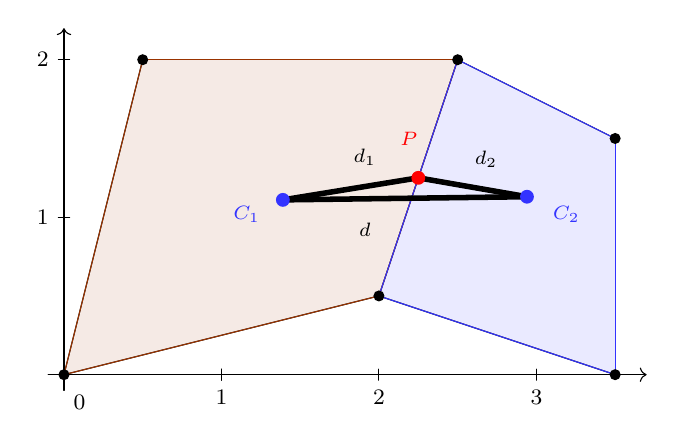
\begin{tikzpicture}[line cap=round,line join=round,x=2cm,y=2cm]
%\draw [color=cqcqcq,dash pattern=on 1pt off 1pt, xstep=1.5cm,ystep=1.5cm] (-0.1,-0.1) grid (3.7,2.2);
\draw[->,color=black] (-0.1,0) -- (3.7,0);
\foreach \x in {,1,2,3}
\draw[shift={(\x,0)},color=black] (0pt,2pt) -- (0pt,-2pt) node[below] {\footnotesize $\x$};
\draw[->,color=black] (0,-0.1) -- (0,2.2);
\foreach \y in {,1,2}
\draw[shift={(0,\y)},color=black] (2pt,0pt) -- (-2pt,0pt) node[left] {\footnotesize $\y$};
\draw[color=black] (0pt,-10pt) node[right] {\footnotesize $0$};
\clip(-0.1,-0.1) rectangle (3.7,2.2);
\fill[color=zzttqq,fill=zzttqq,fill opacity=0.1] (0.5,2) -- (0,0) -- (2,0.5) -- (2.5,2) -- cycle;
\fill[color=ttttff,fill=ttttff,fill opacity=0.1] (2,0.5) -- (3.5,0) -- (3.5,1.5) -- (2.5,2) -- cycle;
\draw (0.5,2)-- (0,0);
\draw (0,0)-- (2,0.5);
\draw (2,0.5)-- (3.5,0);
\draw (3.5,0)-- (3.5,1.5);
\draw (0.5,2)-- (2.5,2);
\draw (2.5,2)-- (3.5,1.5);
\draw (2.5,2)-- (2,0.5);
\draw [color=zzttqq] (0.5,2)-- (0,0);
\draw [color=zzttqq] (0,0)-- (2,0.5);
\draw [color=zzttqq] (2,0.5)-- (2.5,2);
\draw [color=zzttqq] (2.5,2)-- (0.5,2);
\draw [color=ttttff] (2,0.5)-- (3.5,0);
\draw [color=ttttff] (3.5,0)-- (3.5,1.5);
\draw [color=ttttff] (3.5,1.5)-- (2.5,2);
\draw [color=ttttff] (2.5,2)-- (2,0.5);
\draw [line width=2pt] (1.39,1.11)-- (2.94,1.13);
\draw [line width=2pt] (1.39,1.11)-- (2.25,1.25);
\draw [line width=2pt] (2.25,1.25)-- (2.94,1.13);
\begin{scriptsize}
\fill [color=black] (0.5,2) circle (2.0pt);
\fill [color=black] (0,0) circle (2.0pt);
\fill [color=black] (2,0.5) circle (2.0pt);
\fill [color=black] (2.5,2) circle (2.0pt);
\fill [color=black] (3.5,0) circle (2.0pt);
\fill [color=black] (3.5,1.5) circle (2.0pt);
\fill [color=ffqqqq] (2.25,1.25) circle (2.5pt);
\draw[color=ffqqqq] (2.19,1.5) node {$P$};
\fill [color=ttttff] (1.39,1.11) circle (2.5pt);
\draw[color=ttttff] (1.16,1.02) node {$C_1$};
\fill [color=ttttff] (2.94,1.13) circle (2.5pt);
\draw[color=ttttff] (3.19,1.02) node {$C_2$};
\draw[color=black] (1.91,0.92) node {$d$};
\draw[color=black] (1.91,1.38) node {$d_1$};
\draw[color=black] (2.68,1.37) node {$d_2$};
\end{scriptsize}
\end{tikzpicture}
    \caption{Skewness.}
    \label{fig:skewness}
\end{figure}


%    In contrast to the non orthogonality property, this property cannot be numerically \textbf{fixed}. As consequence, it is necessary to have meshes with the lowest skewness possible. It can happen that bad skewness brings to remeshing all the domain. Good skewness values (in OpenFOAM syntax) are: $1 - 8$. 

\subsection{3D mesh} \label{sec:3Dmesh}
The geometry (given in \verb|.stl| format) is converted into 3D mesh\cprotect\footnote{The 2D mesh is already given as \verb|blockMesh| file and its properties are:
\begin{itemize}
    \item \textbf{Skewness}: max $0.84302$. 
    \item \textbf{Non orthogonality}: max: $39.635$ average: $16.5967$. 
\end{itemize}} with OpenFOAM \verb|snappyHexMesh| functions. The meshing procedure followed in OpenFOAM are:
\begin{itemize}
    \item \textbf{Surface features generation with} \verb|surfaceFeatures| This step allows extracting important features from the geometry e.g. important edges and/or important areas in the mesh where it is needed more accuracy (the more the control volumes the more the accuracy, not considering numerical discretization). \verb|surfaceFeaturesDict| sets the commands to follow for the features generation, the main ones are the splitter edges.
    \item \textbf{Mesh generation with} \verb|snappyHexMesh|\cprotect\footnote{The 2D mesh and the 3D mesh follow 2 different tracks: the 2D mesh is based on already existing mesh points (using \verb|blockMesh|); the 3D mesh is based on the computation of the control volumes' points through an optimization algorithm (using \verb|snappyHexMesh|).} This step has 3 substeps:
        \begin{itemize}
            \item \verb|castellatedMesh| This substep allows the removing of blocks that are inside the geometry. The result is a raw block mesh that surrounds the body 
            \item \verb|snap| This substep allows the projection of the raw mesh onto the body surface. 
            \item \verb|addLayers| This last substep allows the inflation of the control volumes close to the surface with smaller control volumes.
        \end{itemize}
\end{itemize}

Coding the meshing steps, it is important to keep in mind the CPU power available - maximum number of control volumes to have good results in appreciable time - and  physical phenomenon to study - shock waves, vortex shedding and flames need more accurate meshes than an airfoil studied with potential flow theory -.   

With respect to these points, since the simulation deals with a hydrocarbon combustion, it is needed to have a good mesh close to the injector position - in order to track better the particles motion -, close to the splitter - where there is a discrete complexity in the geometry and there is the impingement of hydrocarbon particles with the wall film layer - and after the splitter (bluff body) where it is present vortex shedding phenomena. 

With respect to the numerics and topology, it is set a smooth layer transition among the splitter, the combustion region and the combustor case (the layer passes from a level $4$ close to the splitter to level $3$ close to the case). 

At the end of the meshing process the 3D mesh is checked through \verb|checkMesh| and its properties are:
\begin{itemize}
    \item \textbf{Skewness}: max: $1.9082$.
    \item \textbf{Non orthogonality}: max: $64.8094$ average: $7.20918$.
\end{itemize}

The max skewness value is acceptable and also the non orthogonality values are good. The 3D mesh is composed by hexahedron (geometry that works best in OpenFOAM), polyhhedra and prisms. 

\newpage

% PAGE MANAGEMENT
% saving page number
\newcounter{lastPage}
\addtocounter{lastPage}{\thepage}
% changing page numbering for the results figures
\setcounter{page}{1}
\renewcommand{\thepage}{MSH-\roman{page}}

\begin{figure}[!h]
  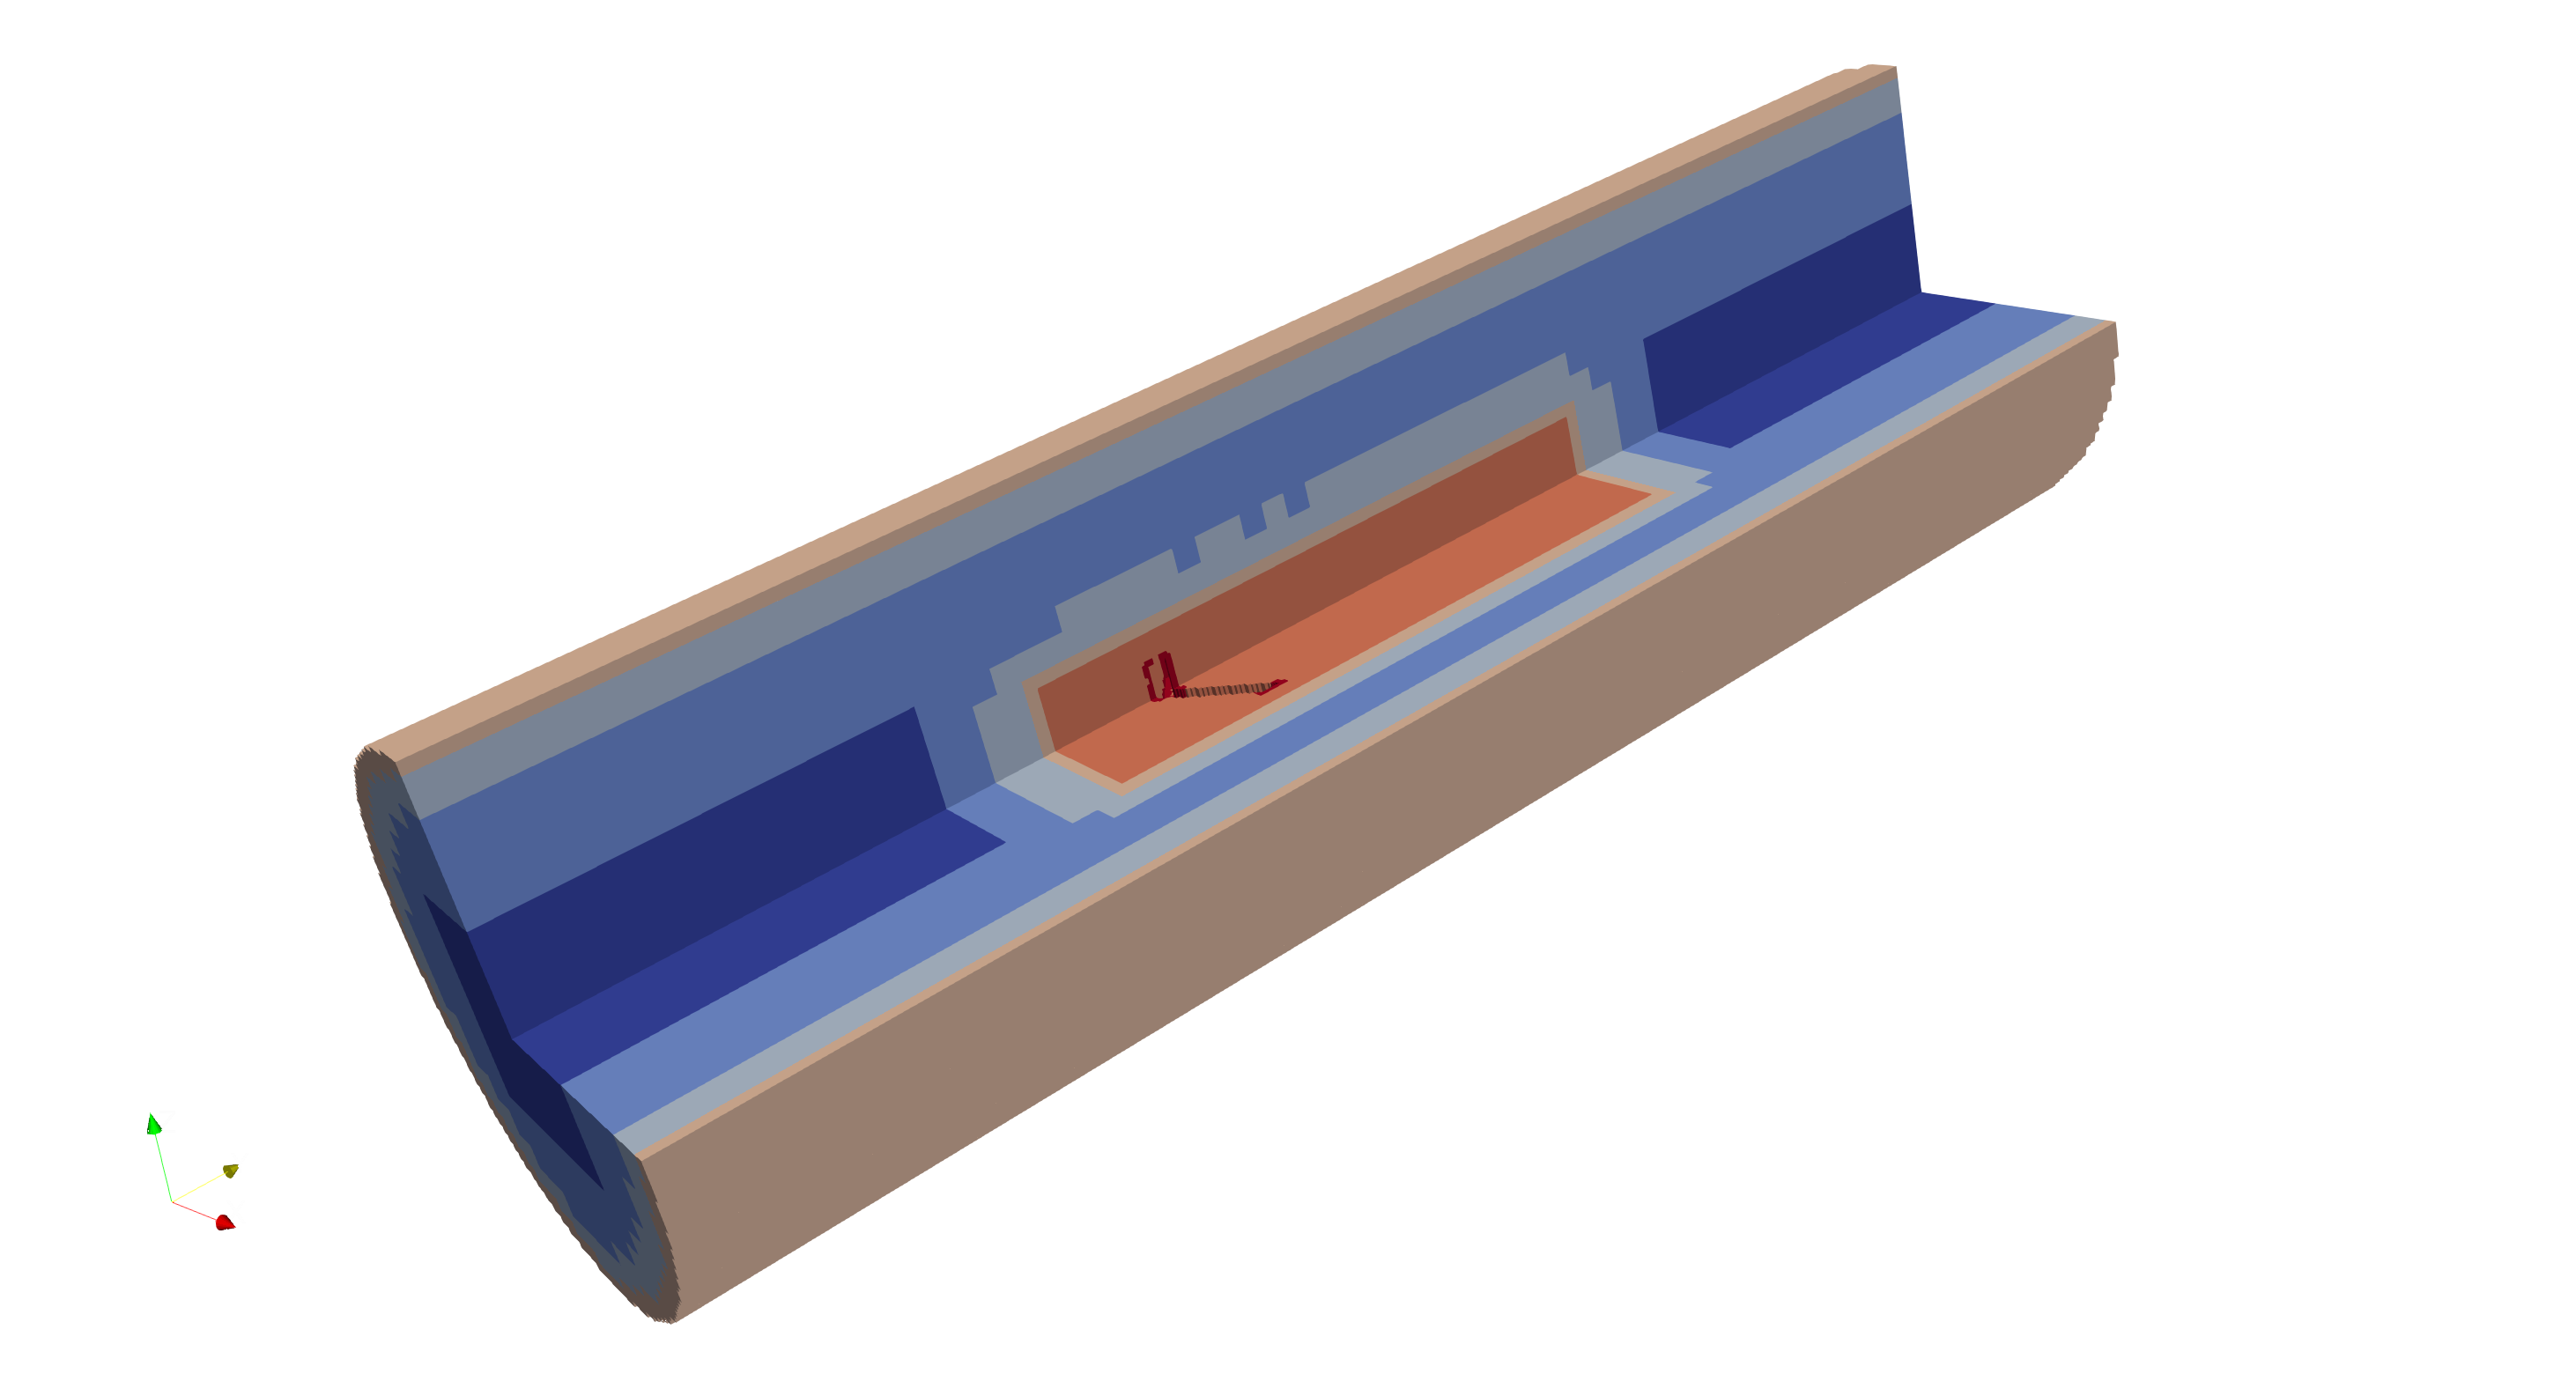
\includegraphics[width=\textwidth]{latexFIGS/figs/mesh3D.png}
    \caption[3D mesh.]{3D mesh. Cell layers where identified with different colors. Due to the available computational power, it has been decided to use a lower number of cells in order to reach an acceptable solution in the shortest time possible.} 
  \label{fig:mesh3D}
\end{figure}

\begin{figure}[!h]
    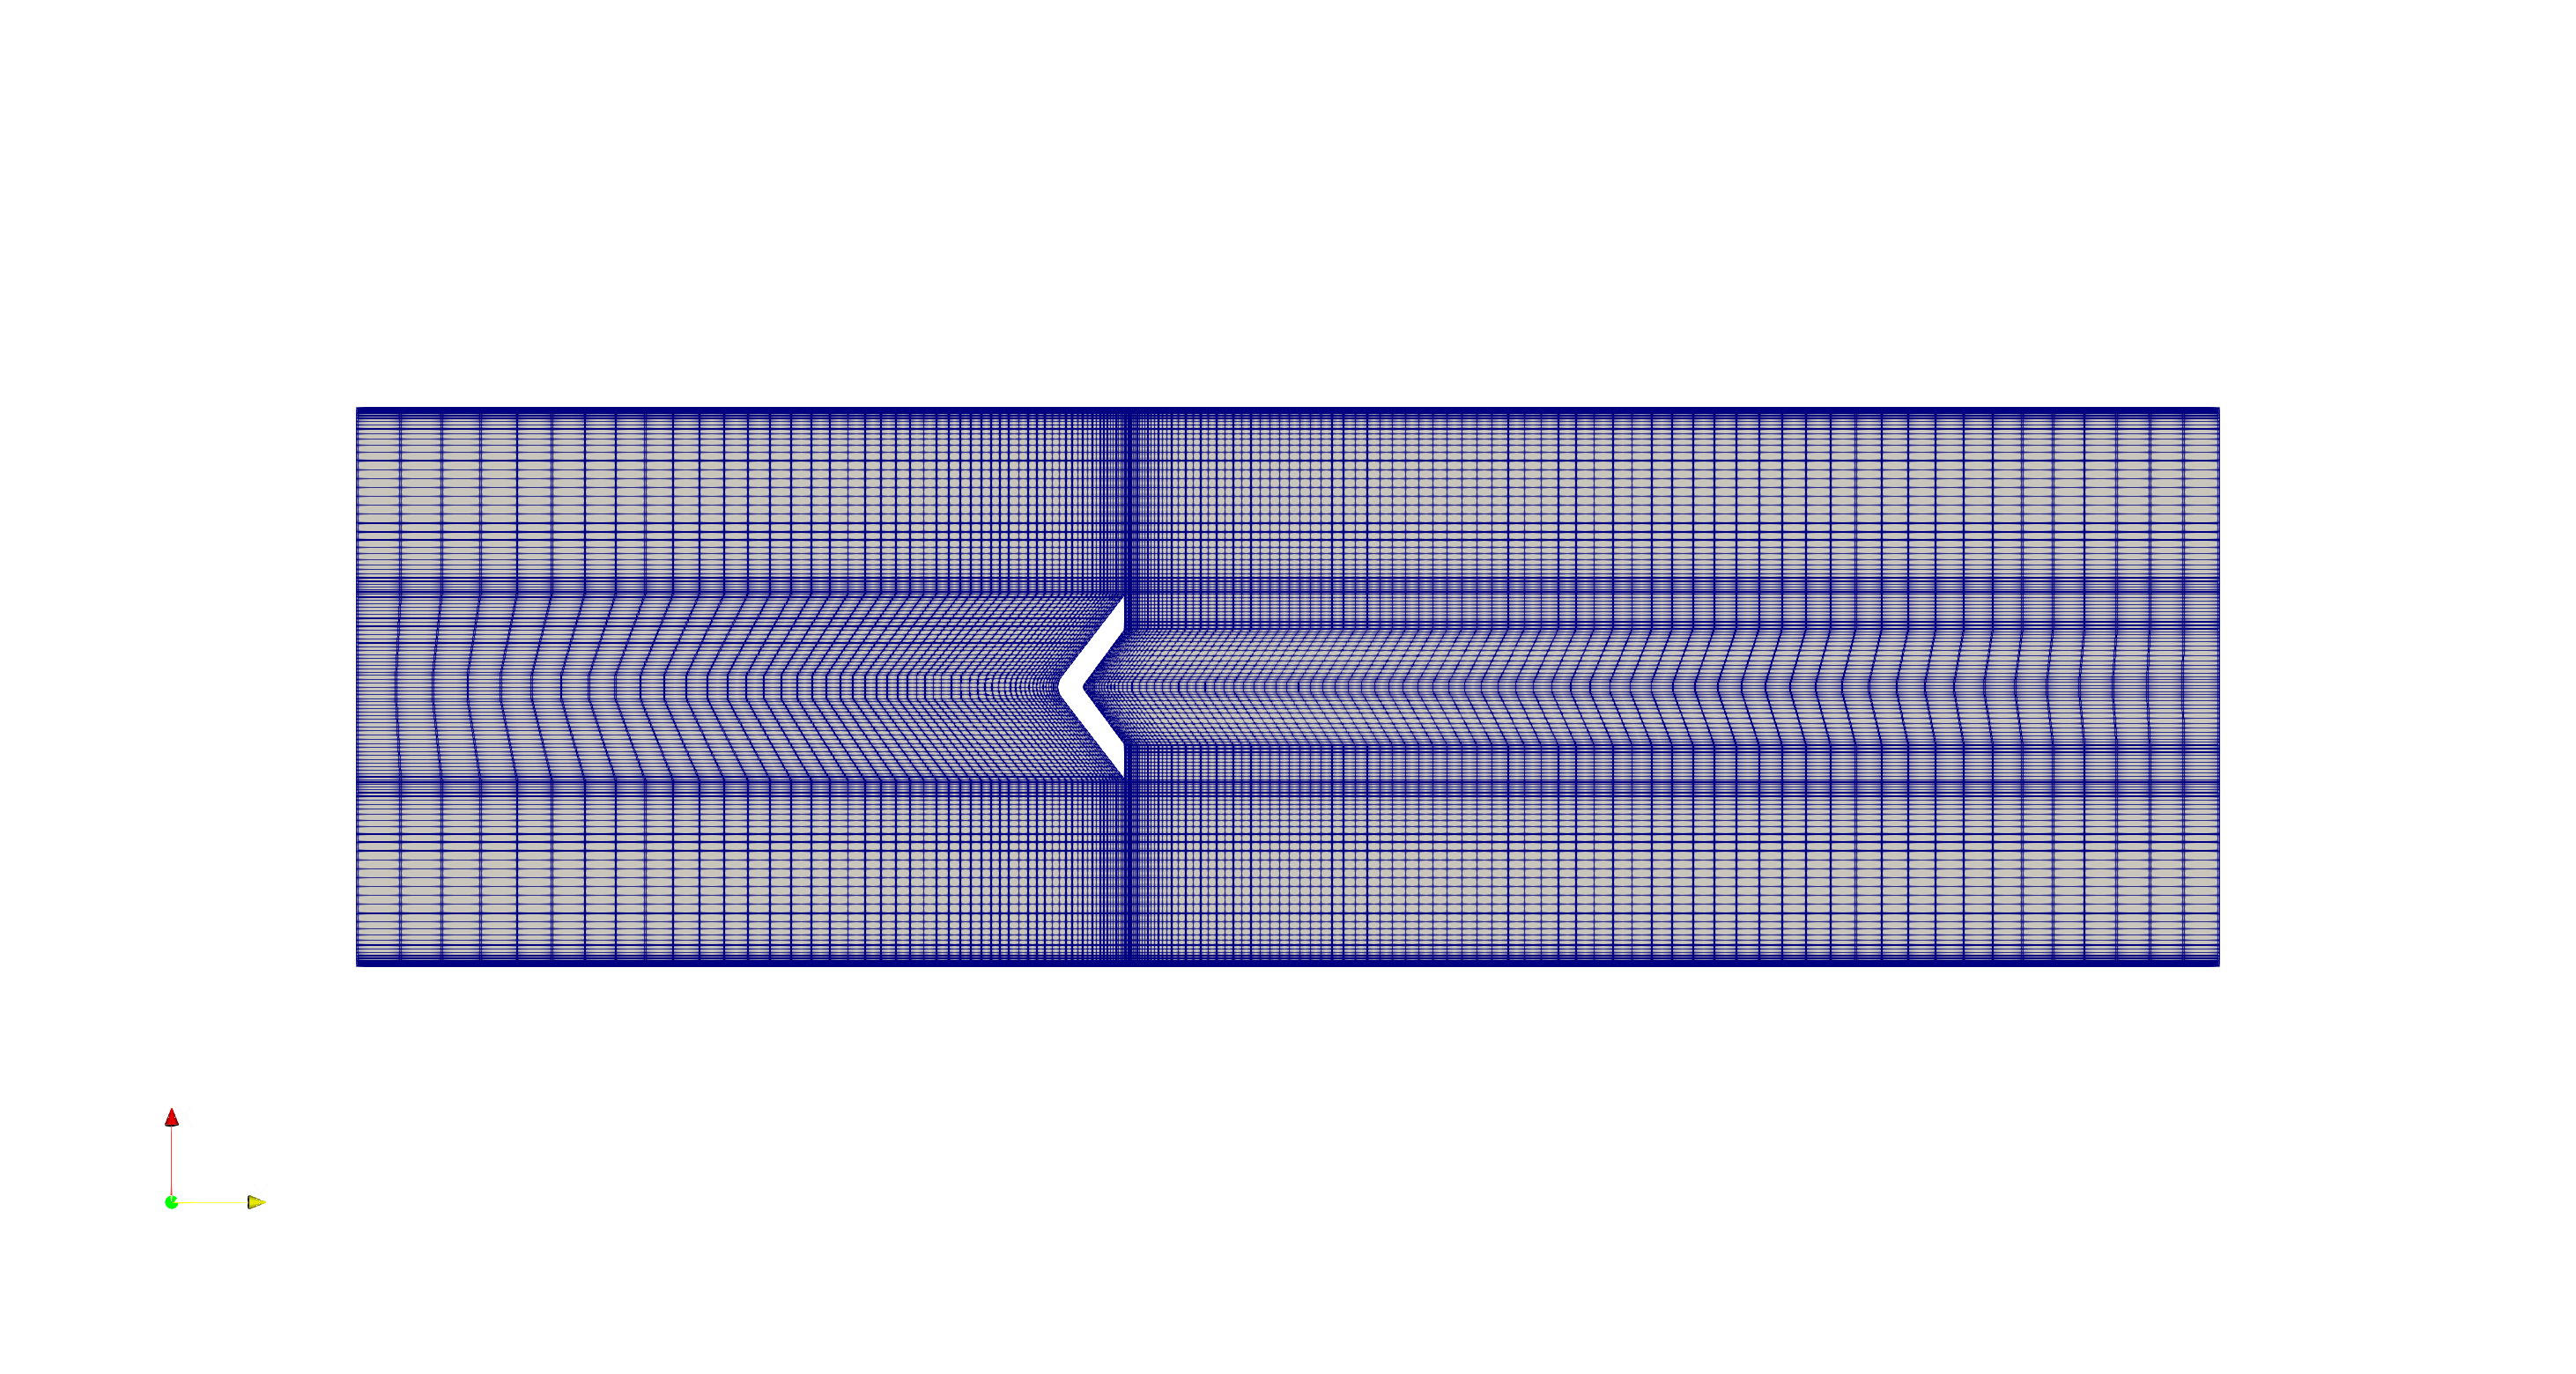
\includegraphics[width=\textwidth]{latexFIGS/figs/mesh2D.png}
    \caption{2D mesh.}
    \label{fig:mesh2D}
\end{figure}

    \newpage
    % !TEX root = ~/OpenFOAM/antoniopucciarelli-9/run/LABS/thermochemical_CFD/main.tex

% INCOMPRESSIBLE CASE 
\section{Incompressible flow - $\mathtt{Lab02}$}

    \renewcommand{\thepage}{\arabic{page}}
    \setcounter{page}{\thelastPage}

All the properties relative to the incompressible flow solvers - \verb|SIMPLE|, \verb|PISO| and \verb|PIMPLE| - are described in detail in~\ref{app:app1}. 

%\subsection{$t$ discretization in OpenFOAM}
%In \verb|PISO/PIMPLE| the time advancing is made in order to discretize the time derivative. As result, the $t$ advancing in the \verb|PISO/PIMPLE| solver has a physical meaning. The contrary is for the \verb|SIMPLE| solver where, in the \verb|fvSchemes|, the time discretization is absent (Listing~\ref{list:ddtSchemes}). In \verb|SIMPLE|, the $t$ advancement is essentially a controller for an additional loop over the predictor-corrector steps. As result, the previous step gives us a better estimate of $p^* - \boldsymbol{u}^*$ used for the numerical problem assembly.

%\begin{lstlisting}[caption = $\mathtt{combustorSimple/system/fvSchemes}$ time discretization., label = list:ddtSchemes]
%ddtSchemes  // time derivative discretization 
%    {       // no need of temporal discretization in SIMPLE algorithm
%        default steadyState; // => no time stencil 
%    }
%\end{lstlisting}

%\cprotect\subsection{\verb|PISO| vs \verb|PIMPLE|}
%The main difference between these two models consists in the \textbf{outer} correction. \verb|PISO| does not have outer correctors. The outer corrector loop consists in a correction of $p^* - \boldsymbol{u}^*$ used in the predictor step\cprotect\footnote{Solved if \verb|momentumPredictor yes;| in \verb|applications/solvers/incompressible/simpleFoam| with check on \verb|simple.momentumPredictor()|.}. This allows, relating all the process to the $\boldsymbol{u}$ at the previous outer corrector step, to find a much more correct estimate of $\boldsymbol{u}$ at the new time step due to the fact that we have a better system formulation (based on $p - \boldsymbol{u}$ already estimated at the end of the previous predictor-corrector steps) that makes the problem treatment much like an \textbf{implicit} method. The \textbf{outer} correction step is very computational demanding but, at the same time, it is possible using $\Delta t$ such that $Co > 1$. So choosing between \verb|PISO| and \verb|PIMPLE|, other than convergence and numerics, can be described with time step iterations\cprotect\footnote{It is important to keep in mind that \verb|pisoFoam| in OpenFOAM does not change the $\Delta t$. In order to solve this issue - so keeping $Co < 1$ and allowing $\Delta t$ to change -, it is used running \verb|pimpleFoam| in \verb|PISO| mode. Of course, the number of outer corrector for \verb|pimpleFoam| in \verb|PISO| mode is $0$.}.  

%\subsubsection{Courant-Friedrichs-Lewy} 
%In time marching problems, the CFL test allows to find a proper time step in order to link the \textbf{spatial} stencil with the \textbf{temporal} stencil, Figure~\ref{fig:CFL}.

%\begin{figure}[h!]
\vspace*{-1.5cm}
\centering
\definecolor{ttttff}{rgb}{0.2,0.2,1}
\definecolor{qqqqff}{rgb}{0,0,1}
\begin{tikzpicture}[line cap=round,line join=round,x=1cm,y=1cm]
\draw[->,color=black] (1,0) -- (7,0);
\foreach \x in {1,2,3,4,5,6,7}
\draw[->,color=black] (1,-0.1) -- (1,2);
\draw[shift={(1,0)},color=black] (2pt,0pt) -- (-2pt,0pt) node[left] {\footnotesize ${t}$};
\draw[shift={(1,1)},color=black] (2pt,0pt) -- (-2pt,0pt) node[left] {\footnotesize $t + \Delta t$};
\clip(0.9,-0.89) rectangle (7,3.57);
\draw [line width=2pt,dash pattern=on 1pt off 1pt,domain=-0.37:7.9] plot(\x,{(--4-0*\x)/4});
\draw [line width=2pt] (2,0)-- (4,0);
\draw [line width=2pt] (4,0)-- (6,0);
\draw [line width=1.2pt,dotted] (2,0)-- (4,1);
\draw [line width=1.2pt,dotted] (4,1)-- (6,0);
\draw [line width=1.2pt,color=ttttff] (4,1)-- (4.82,0);
\draw [line width=1.2pt,color=ttttff] (4,1)-- (2.83,0);
\begin{scriptsize}
\fill [color=black] (2,0) circle (2pt);
    \draw[color=black] (2.2,-0.1) node[below] {$x_{(t)} - \Delta x_{(t)}$};
\fill [color=black] (4,0) circle (2pt);
    \draw[color=black] (4.09,-0.09) node[below] {$x_{(t)}$};
\fill [color=black] (6,0) circle (2pt);
    \draw[color=black] (6.21,-0.1) node[below] {$x_{(t)} + \Delta x_{(t)}$};
\fill [color=qqqqff] (4,1) circle (2pt);
    \draw[color=qqqqff] (4.26,1.12) node[above] {$x_{(t + \Delta t)}$};
\end{scriptsize}
\end{tikzpicture}
    
    \caption{CFL, spatial and temporal stencils.}
    \label{fig:CFL}

\end{figure}


%As result, it is ensured that the $p - \boldsymbol{u}$ fields are physically related to the previous time steps. Of course, using $Co < 1$ does not guarantee achieving convergence; the convergence is related also to the discretization schemes and the correctors - so mainly, how the problem is solved -. The CFL condition is expressed as \cite[Ch. 13]{quarteroni2012numerical}:

%\begin{equation}
%    max_{\Omega} \Bigg( \frac{\big| \boldsymbol{u} \big| \ \Delta t}{\Delta x} \Bigg) < 1.0
%    \label{eqn:CFL}
%\end{equation}

%\noindent From (\ref{eqn:CFL}), $\Delta t$ is computed. There are methods, such as \verb|PIMPLE|, that allow relaxation on this stencils constraint; this is mainly related to the way the solution is computed. $Co > 1$ acts as a filter on the solution: physics with time scales shorter than $\Delta t$ are not seen in the final solution e.g. vortex shedding. In addition, for $Co > 1$ the time discretization error propagates on the solution; the last time step is the initial condition for the new time step. In OpenFOAM the Courant-Friedrichs-Lewy conditions is expressed through \verb|maxCo|. 

%\subsection{Under relaxation}
%The under relaxation consists in changing the value of a computed field in order to smooth out convergence. The under relaxation process followed in many codes is the \textbf{Patankar} model~\cite[Ch. 14.1]{moukalled2016finite}, that consists in an explicit (\ref{eqn:expPATANKAR}) and an implicit (\ref{eqn:PATANKAR}) formulation:
%\begin{align}
%    \phi_{j + 1}^{relaxed} & = \phi_{j} + \alpha_{\phi} \ \big( \phi_{j + 1} - \phi_{j} \big) \label{eqn:expPATANKAR} \\ 
%    \frac{a_C}{\lambda_{\phi}} \ \phi_{C_{j + 1}} + \sum_F a_F \ \phi_{F_{j + 1}} & = b_C + \frac{1 - \lambda_{\phi}}{\lambda_{\phi}} \ a_C \ \phi_{C_j} 
%    \label{eqn:PATANKAR}
%\end{align}

%\noindent This model relies on $\alpha_{\phi}$ that is the relaxation parameter of the $\phi$ field. The most used $\alpha_{\phi}$ values are: $\alpha_{\boldsymbol{u}} \approx 0.7$ and $\alpha_{p} \approx 0.3$. Now, having explained the relaxation model, it is necessary to relate it to the different algorithms. The under relaxation is not present in the \verb|PISO| algorithm; this because the under relaxed field without outer corrector loop generates a not physical field, so it should not became an output of the solver. As this said, the \verb|PISO| algorithm outputs directly the $p$ field and the corrected $\boldsymbol{u}$ field ($\boldsymbol{u} = \boldsymbol{u}_{(p, \ \boldsymbol{u}^*)}$). The other algorithms, \verb|SIMPLE| and \verb|PIMPLE|, allow using under relaxation. The under relaxation parameters are expressed in \verb|system/fvSolution| with \verb|relaxationFactors| and it can be explicit on a field with \verb|fields| setting or implicit in the equations with \verb|equations| setting.

\subsection{Problem setup}
\subsubsection{Boundary conditions}
The boundary conditions to be set are relative to the $p-\boldsymbol{u}$ and the turbulence model. Since the problem is incompressible, $p$ is expressed as $\frac{p}{\rho}$ in order to facilitate the computation\cprotect\footnote{This brings to set the \verb|p| boundary conditions dictionary \verb|dimensions [0 2 -2 0 0 0 0];|.}. The internal field for $p-\boldsymbol{u}$ is $0$. 

\paragraph{Turbulence model}
Since the \verb|RAS| model uses the $\kappa-\varepsilon$ tubulence model~\cite[Ch. 10.4]{pope2000turbulent}, set in \verb|constant| with \verb|momentumTransport|, it is needed to set up $\kappa-\varepsilon-\nu_t$ boundary conditions. 

\subparagraph{$\varepsilon$} For $\varepsilon$ (turbulent dissipation rate $\frac{1}{2} \ \nu < s_{ij}^{\prime} s_{ij}^{\prime} >$\footnote{$s_{ij}^{\prime} = \frac{1}{2} \big( \frac{\partial u_i^{\prime}}{\partial x_j}  + \frac{\partial u_j^{\prime}}{\partial x_i} \big)$, deviatoric part of $\boldsymbol{\nabla \ u}^{\prime} $}), the inlets have the same turbulence setup \verb|turbulentMixingLengthDissipationRateInlet| and the \verb|mixingLength| is fixed\footnote{Key parameter for the computation of $\nu_t$.}. The walls are modeled with a wall function model: \verb|epsilonWallFunction|. The outlet is set to \verb|zeroGradient| (it means that $\varepsilon$ does not change \textbf{in space} at the outlet). 

\subparagraph{$\kappa$} The $\kappa$ (turbulent kinetic energy $\sum_i < u_i^{\prime} u_i^{\prime} >$) follows the same philosophy of $\varepsilon$ - turbulent model at the inlet with \verb|turbulentIntensityKineticEnergyInlet|, \verb|kqrWallFunction| at the wall and \verb|zeroGradient| at the outlet -.

\subparagraph{$\nu_t$} Although $\nu_t$ (turbulent viscosity to be added to the molecular viscosity $\nu$ described in \verb|constant/transportProperties|) is completelly described by $\kappa-\varepsilon$, it is possible to impose boundary conditions on it. $\nu_t$ at the walls is modelled with a wall function model \verb|nutkWallFunction|; the rest of the field is directly computed via $\kappa-\varepsilon$ model.  

\subsubsection{Schemes}
\cprotect\paragraph{\verb|fvSchemes|} All the fields are discretized with a second order interpolation based on Gauss integration. The laplacian field and the surface normal gradient schemes are set to \verb|corrected| that means the non orthogonality property is corrected via correctors (that allows sticking with a second order accuracy model).  

\cprotect\paragraph{\verb|fvSolution|}
In the unsteady solver it is described the number of outer correctors, \verb|nOuterCorrectors|, and the number of internal correctors, \verb|nCorrectors|\cprotect\footnote{\verb|nNonOrthogonalCorrectors 0;| because the mesh has low non orthogonality.}. Turbulence is set as present in all the outer correctors with \verb|turbOnFinalIterOnly no;|, this allows to have a better evaluation of $\nu_t$. It is set the relaxation factors only for \verb|combustorPimpleCFL15| in order to guarantee convergence due to \verb|maxCo 15;|. In \verb|combustorPimpeCFL1| there are not present any relaxation factors, this partially because \verb|maxCo 1;| that allows less changes of the solution over the time steps. The \verb|combustorPimple1| set up is not like \verb|PISO| because there are $100$ outer correctors (\verb|PISO| has none). 

For the error check it has been used \verb|tolerance| and \verb|relTol| both in the iterative methods, used for the computation of the fields, and also on the outer correctors (that can be seen as a refinement process of the $p^* - \boldsymbol{u}^*$ variables). Solvers are based on \verb|GAMG|\footnote{Generalised geometric algebraic multi grid: used for the momentum equation solution (asymmetric matrix).} and \verb|smoothSolver|\cprotect\footnote{Solver that uses a smoother: in the cases it is used for the continuity equation - Poisson equation - (symmetric matrix). Of course the smoother model has to be described with \verb|smoothSolver|.}. In the \verb|combustorPimpleCFL15|, the \verb|*Final|\cprotect\footnote{This is a way of treating differently the last outer corrector cycle. The last outer corrector cycle depends on \verb|nOuterCorrectors| or if the outer corrector tolerances are satisfied.} relative tolerances (\verb|relTol|) are set to $0$; this in order to guarantee convergence using an error check based on \verb|tolerance|. 

\subsection{Post processing}
The post processing functions are declared in \verb|system/controlDict|. The main values extracted are the solution's initial residuals, the forces on the splitter, the $y^+$ in the boundarly layer close to the walls and the $U_y$ velocity at $y = 100 mm$. 

\subsection{Results}
\cprotect\subsubsection{\verb|combustorSimple|}
It is possible to see that \verb|simpleFoam| does not reach convergence. This is a \textbf{numerical error} related to the body geoemtry: it is a bluff body. As result the solution oscillates between 2 \textit{numerical} admissible solutions. The point here is that it is trying to simulate an unsteady phenomena with a steady solver. 

There are not problems with the drag force computation. Since the geometry is symmetric, the drag force over the \textit{fitious} time steps is the same. 

\cprotect\subsubsection{\verb|combustorPimpleCFL1|}
With \verb|maxCo 1;| constraint, the results represent the vortex shedding after the splitter. Since the non physical initial conditions, the drag force has a large escursion the first time steps but then it settles down to a constant value. This constant value of drag force is made by the low changing pressure field around the splitter, although the vortex shedding in time. 

\cprotect\subsubsection{\verb|combustorPimpleCFL15|}
With \verb|max Co 15;| constraint, in this case the vortex shedding phenomena starts to show later in the solution. This is related to the filtering action of using a stable - outer corrector - solver with unlinked time-space discretization. As in the other solvers, the first time steps are affected by large escursion in the drag force due to the convergence of the internal field.  

\newpage

% PAGE MANAGEMENT
% saving page number
%\newcounter{lastPage}
%\addtocounter{lastPage}{\thepage}
\setcounter{lastPage}{\thepage}
% changing page numbering for the results figures
\setcounter{page}{1}
\renewcommand{\thepage}{INC-\roman{page}}

\begin{figure}[!h]
    \centering
    \import{latexFIGS/lab02/}{residuals.pgf}
    \caption{Incompressible cases: residuals.}
    \label{fig:Res}
\end{figure}

\begin{figure}[!h]
    \centering
    \import{latexFIGS/lab02/}{Uy.pgf}
    \caption{Incompressible cases: $U_y$.}
    \label{fig:Uy}
\end{figure}

\begin{figure}[!h]
    \centering
    \import{latexFIGS/lab02/}{forces.pgf}
    \caption{Incompressible cases: forces.}
    \label{fig:forces}
\end{figure}

\begin{figure}[!h]
    \centering
    \import{latexFIGS/lab02/}{yPlus.pgf}
    \caption{Incompressible cases: $y^+$.}
    \label{fig:yPlus}
\end{figure}

\begin{figure}[!h]
    \includegraphics[width=\textwidth]{latexFIGS/figs/combustorPimple15.png}
    \caption{Velocity profile for combustor with CFL < 15.}
\end{figure}

\clearpage

    \newpage
    % !TEX root = ~/OpenFOAM/antoniopucciarelli-9/run/LABS/thermochemical_CFD/main.tex

\section{Compressible flow - $\mathtt{Lab04}$}
    
    \renewcommand{\thepage}{\arabic{page}}
    \setcounter{page}{\thelastPage}
In~\ref{app:app2} are described the main equations, concepts and possible OpenFOAM implementation for compressible flows.

%    \subsection{Energy equation}
%With respect to the incompressible case, the compressible case enables the changes in $\rho$ of the fluid. This new degree of freedom in the system has to be treated with care using the energy equation. The energy equation has different forms that suit best for defined physical behaviours in the system\footnote{$h$ is the specific enthalpy, $e$ is the specific internal energy, $K$ is the total kinetic energy and $E$ is the total energy.}:

%{\small
%\begin{align} 
%    \frac{\partial \rho e}{\partial t} + \boldsymbol{\nabla} \cdot \big( \rho \boldsymbol{u} e \big) + \frac{\partial \rho K}{\partial t} + \boldsymbol{\nabla} \cdot \big( \rho \boldsymbol{u} K \big) + \boldsymbol{\nabla} \cdot \big( \boldsymbol{u} p \big) = - \boldsymbol{\nabla} \cdot \boldsymbol{q} + \boldsymbol{\nabla} \cdot \big( \boldsymbol{\tau} \cdot \boldsymbol{u} \big) + \rho r + \rho \boldsymbol{g} \cdot \boldsymbol{u} \label{eqn:heqn} \\  
%    \frac{\partial \rho h}{\partial t} + \boldsymbol{\nabla} \cdot \big( \rho \boldsymbol{u} h \big) + \frac{\partial \rho K}{\partial t} + \boldsymbol{\nabla} \cdot \big( \rho \boldsymbol{u} K \big) - \frac{\partial p}{\partial t} = - \boldsymbol{\nabla} \cdot \boldsymbol{q} + \boldsymbol{\nabla} \cdot \big( \boldsymbol{\tau} \cdot \boldsymbol{u} \big) + \rho r + \rho \boldsymbol{g} \cdot \boldsymbol{u} \label{eqn:eeqn} \\  
%    \frac{\partial \rho E}{\partial t} + \boldsymbol{\nabla} \cdot \big( \rho \boldsymbol{u} E \big) + \boldsymbol{\nabla} \cdot \big( \boldsymbol{u} p \big) = - \boldsymbol{\nabla} \cdot \boldsymbol{q} + \boldsymbol{\nabla} \cdot \big( \boldsymbol{\tau} \cdot \boldsymbol{u} \big) + \rho r + \rho \boldsymbol{g} \cdot \boldsymbol{u} \label{eqn:Eeqn}  
%\end{align}. 
%}

%One of the most used energy equation is in the $h$ formulation~\cite[Ch. 11]{ferziger2002computational}. The $h$ formulation uses $h = e + \frac{p}{\rho}$ and $K$ as \textit{thermodynamic} and \textit{mechanical} energy describers. In both $h - e$ formulations, $K$ is always computed; instead in the total energy formulation, $K$ is hidden in $E = e + K$. Most of the energy formulations in OpenFOAM neglect the mechanical part $\boldsymbol{\nabla} \cdot \big( \boldsymbol{\tau} \cdot \boldsymbol{u} \big)$ and $\rho \boldsymbol{g} \cdot \boldsymbol{u}$.  

%In the whole assignment, the compressibility is treated with the $h$ formulation. The reason about this choice relies on the physics of the problem: for a problem with heat flux and with combustion of a non premixed mixture, the $h$ formulation is preferred.

%\subsubsection{$h$ equation in OpenFOAM}
%There are different ways for solving the compressible flow problems. The philosophy stays the same. One of the possible $h$ formulations is described in \verb|rhoPimpleFoam| and the main codes used in it are \verb|pEqn.H|, \verb|UEqn.H|, \verb|EEqn.H| and \verb|rhoPimpleFoam.C|. 

%The main parts of \verb|rhoPimpleFoam.C| are the following: 
%\begin{itemize}
%    \item \textbf{Outer loop}
%    \begin{itemize}
%        \item \textbf{$\rho$ computation} - \verb|rhoEqn.H| - Since $\rho$ is a derived field, it needs to be computed. 
%        \item \textbf{$\boldsymbol{u}$ predictor} - \verb|UEqn.H| - Computation of a first $\boldsymbol{u}$ approximation. 
%        \item \textbf{$h$ equation} - \verb|EEqn.H|\cprotect\footnote{\verb|EEqn.H| uses \verb|dpdt|. \verb|dpdt| is computed in \verb|pEqn.H| with \verb|dpdt = fvc::ddt(p)|.} - Computation of the $h - T$ field through guessed $\rho - p^*$ and the previous predicted $\boldsymbol{u}$. 
%        \item \textbf{Inner loop}
%        \begin{itemize}
%            \item \textbf{$p$ corrector} - \verb|pEqn.H|\cprotect\footnote{The Helmoltz equation can be seen as a Poisson equation with a $\frac{\partial \rho}{\partial t}$ term that is converted in $p$ terms and then treated implicitly.} - Guarantee continuity with Helmolts equation.
%            \begin{itemize}
%                \item \textbf{$\frac{\partial p}{\partial t}$ computation} Computation of $\frac{\partial p}{\partial t}$ needed in $h$ formulation.
%            \end{itemize}
%            \item \textbf{$\rho$ computation/correction} - \verb|rhoEqn.H| - Correcting again $\rho$ field with new $p$ field and the $T$ field from the $h$ equation solution.
%    \end{itemize}
%    \end{itemize}
%    \item \textbf{Convergence check}
%    \item \textbf{Time step advancement}
%    \begin{itemize}
%        \item \textbf{Guessed fields for the new time step} The new time step gets the guessed values from the last time step solutions.
%    \end{itemize}
%\end{itemize}

%\subsubsection{$\psi$ and $\rho$ based model}
%In CFD there are many ways for coupling the energy, pressure, velocity equations and the equation of state. All these ways for the computation of $\rho$ can be separated in 2 families: the pressure based $\psi$ equation and the $\rho$ based equations. 

%\paragraph{$\psi$} The $\psi$ based equations uses an explicit relation between $\rho$ and $p$ through $\psi$. An example is the $\psi$ equation that is based on the equation of the perfect gases, $\psi = \frac{1}{R T}$ such that $\rho = \psi \cdot p$. This family of models are best suitable for the segregated (semi-implicit) method because it is a \textbf{$p$ based} algorithm.

%\paragraph{$\rho$} The $\rho$ based equations are another set of equations that allow the computation of $\rho$ through a $\rho$ dependent PDE or through an equation that does not explicitly relate $\rho$ to $p$ such as the \textbf{Boussinesque approximation} $\Delta \rho = \beta \Delta T$.

\subsection{Problem setup}
\subsubsection{Boundary conditions}
The main changes in the boundary conditions in \verb|0/| folder are:
\subparagraph{$p$} Due to the presence of pressure waves, because the hyperbolic formulation of the problem, the outlet boundary condition has to be changed. As result of this, the outlet allows pressure waves to pass through and it allows also to not over-constraint the problem. So the outlet is set as \verb|waveTransmissive| type and with the pressure field at infinite equal to \verb|internalField|. Of course, the dimension of $p$ has to change because now the problem is no more formulated as $\frac{p}{\rho}$. 
\subparagraph{$\alpha_t$} Due to the compressibility, the problem has to deal with turbulent heat transfer coefficient $\alpha_t$. All the $\alpha_t$ are set as \verb|calculated| except at the walls where it is used a wall function \verb|compressible::alphatWallFunction|\footnote{The use of wall functions in $\kappa$, $\varepsilon$, $\nu_t$ and $\alpha_t$ is related to the fact that the centres of all the nearest control volumes to the walls are at $y^+ > 10$ and so out of the \textbf{viscous subregion}. Being out of this region it is necessary compute with the wall function these values. This will result in exploiting the results of theory: \textbf{log-law} model adoption.}.   
\subparagraph{$T$} Setting $T$ boundary conditions is like setting $h$ boundary conditions, because their relation. The \verb|T| file changes for each problem because different boundary conditions at the walls and the flow field temperature.

\subsubsection{Schemes}
\cprotect\paragraph{\verb|fvSchemes|}
New schemes are added such \verb|div(phi,h)| and \verb|div(phi,K)| that allow to compute $\boldsymbol{\nabla} \cdot \big( \rho \ \boldsymbol{u} \ h \big)$ and $\boldsymbol{\nabla} \cdot \big( \rho \ \boldsymbol{u} \ K \big)$ respectilvely.

\verb|wallDist| is a new function that describes the method used for the \verb|waveTransmissive| type in \verb|p|.

\cprotect\paragraph{\verb|fvSolution|}
The compressible case has to deal also with how to solve the energy equations, so solution schemes and tolerances are declared as well as $p$ and $U$ for $h$.

\cprotect\subsubsection{\verb|thermophysicalProperties|}
This file allows to describe the way the equation of energy is solved and how to compute $\rho$ from the available fields. 
\cprotect\paragraph{\verb|thermoType|}
This part of the dictionary declares how to solve energy and $\rho$ through \verb|hePsiThermo|.
\begin{itemize}
    \item \verb|hePsiThermo| - \verb|type| - allows the usage of the equation of energy base on $h - e$ and the usage of $\psi$ based method for the computation of $\rho$ (so explicitly related to $p$). 
    \item \verb|pureMixture| - \verb|mixture| - allows treating a single mixture in gaseous phase.
    \item \verb|perfectGas| - \verb|equationOfState| - allows using the perfect gas equation $\rho~=~\frac{p}{R T}$ for $\psi$.
    \item \verb|sensibleEnthalpy| - \verb|energy| - allows using the $h$ formulation for the energy equation.
\end{itemize}

\cprotect\paragraph{\verb|mixture|}
This part of the dictionary declares the mixture properties. 

The following \verb|mixture| properties are related to gas propeties:
\begin{itemize}
    \item \verb|specie| sets the molecular weight of the substance - air in this case -.
    \item \verb|thermodynamics| sets the thermodynamics relations between $T$ and $h$; based on constants as expressed in \verb|thermoType -> thermo hConst;|
    \item \verb|transport| sets transport properties of the mixture and are set to \verb|const| in \verb|thermoType -> transport const;|.
\end{itemize}

\verb|dpdt yes;| enables the usage of $\frac{\partial p}{\partial t}$ used in the $h$ formulation. 

\subsection{Post-processing}
All the post-processing functions, except the residual function, print the field with time interval $\Delta t = 0.1 s$ in order to save disk space. 
\cprotect\subsubsection{\verb|MachNo|}
This is a post-process function that enables the computation of Mach field using $Ma = \frac{U}{\sqrt{\gamma R T }}$. 

\subsection{Results}    
\cprotect\subsubsection{\verb|combustorRhoPimple_lowT_lowRe|}
This simulation was set \verb|maxCo 5.0;|. Vortex shedding is present in the field. With respect to the other fields, pressure waves travel at lower speed, this brings to a longer time for the velocity to change.   

\cprotect\subsubsection{\verb|combustorRhoPimple_highT_lowRe|}
This simulation starts to show instability effects from the last few steps of the simulation. The pressure wave speed\footnote{$c = \sqrt{\gamma \ R \ T}$.} is higher than in the \verb|combustorRhoPimple_lowT_lowRe| case.

\cprotect\subsubsection{\verb|combustorRhoPimple_hightT_highRe|}
As the previous simulation, flow instability effects start to be present in the final solution steps. 

\newpage

% PAGE MANAGEMENT
% saving page number
\setcounter{lastPage}{\thepage}
% changing page numbering for the results figures
\setcounter{page}{1}
\renewcommand{\thepage}{COM-\roman{page}}

\begin{figure}[!h]
    \centering
    \import{latexFIGS/lab04/}{residuals.pgf}
    \caption{Compressible cases: residuals.}
    \label{fig:residualComp}
\end{figure}

\begin{figure}[!h]
    \centering
    \import{latexFIGS/lab04/}{T.pgf}
    \caption{Compressible cases: $T$ profile at $y = 100mm$.}
    \label{fig:Tcomp}
\end{figure}

\begin{figure}[!h]
    \centering
    \import{latexFIGS/lab04/}{Uy.pgf}
    \caption{Compressible cases: $U_y$ profile at $y = 100mm$.}
    \label{fig:UyCOMP}
\end{figure}

\begin{figure}[!h]
    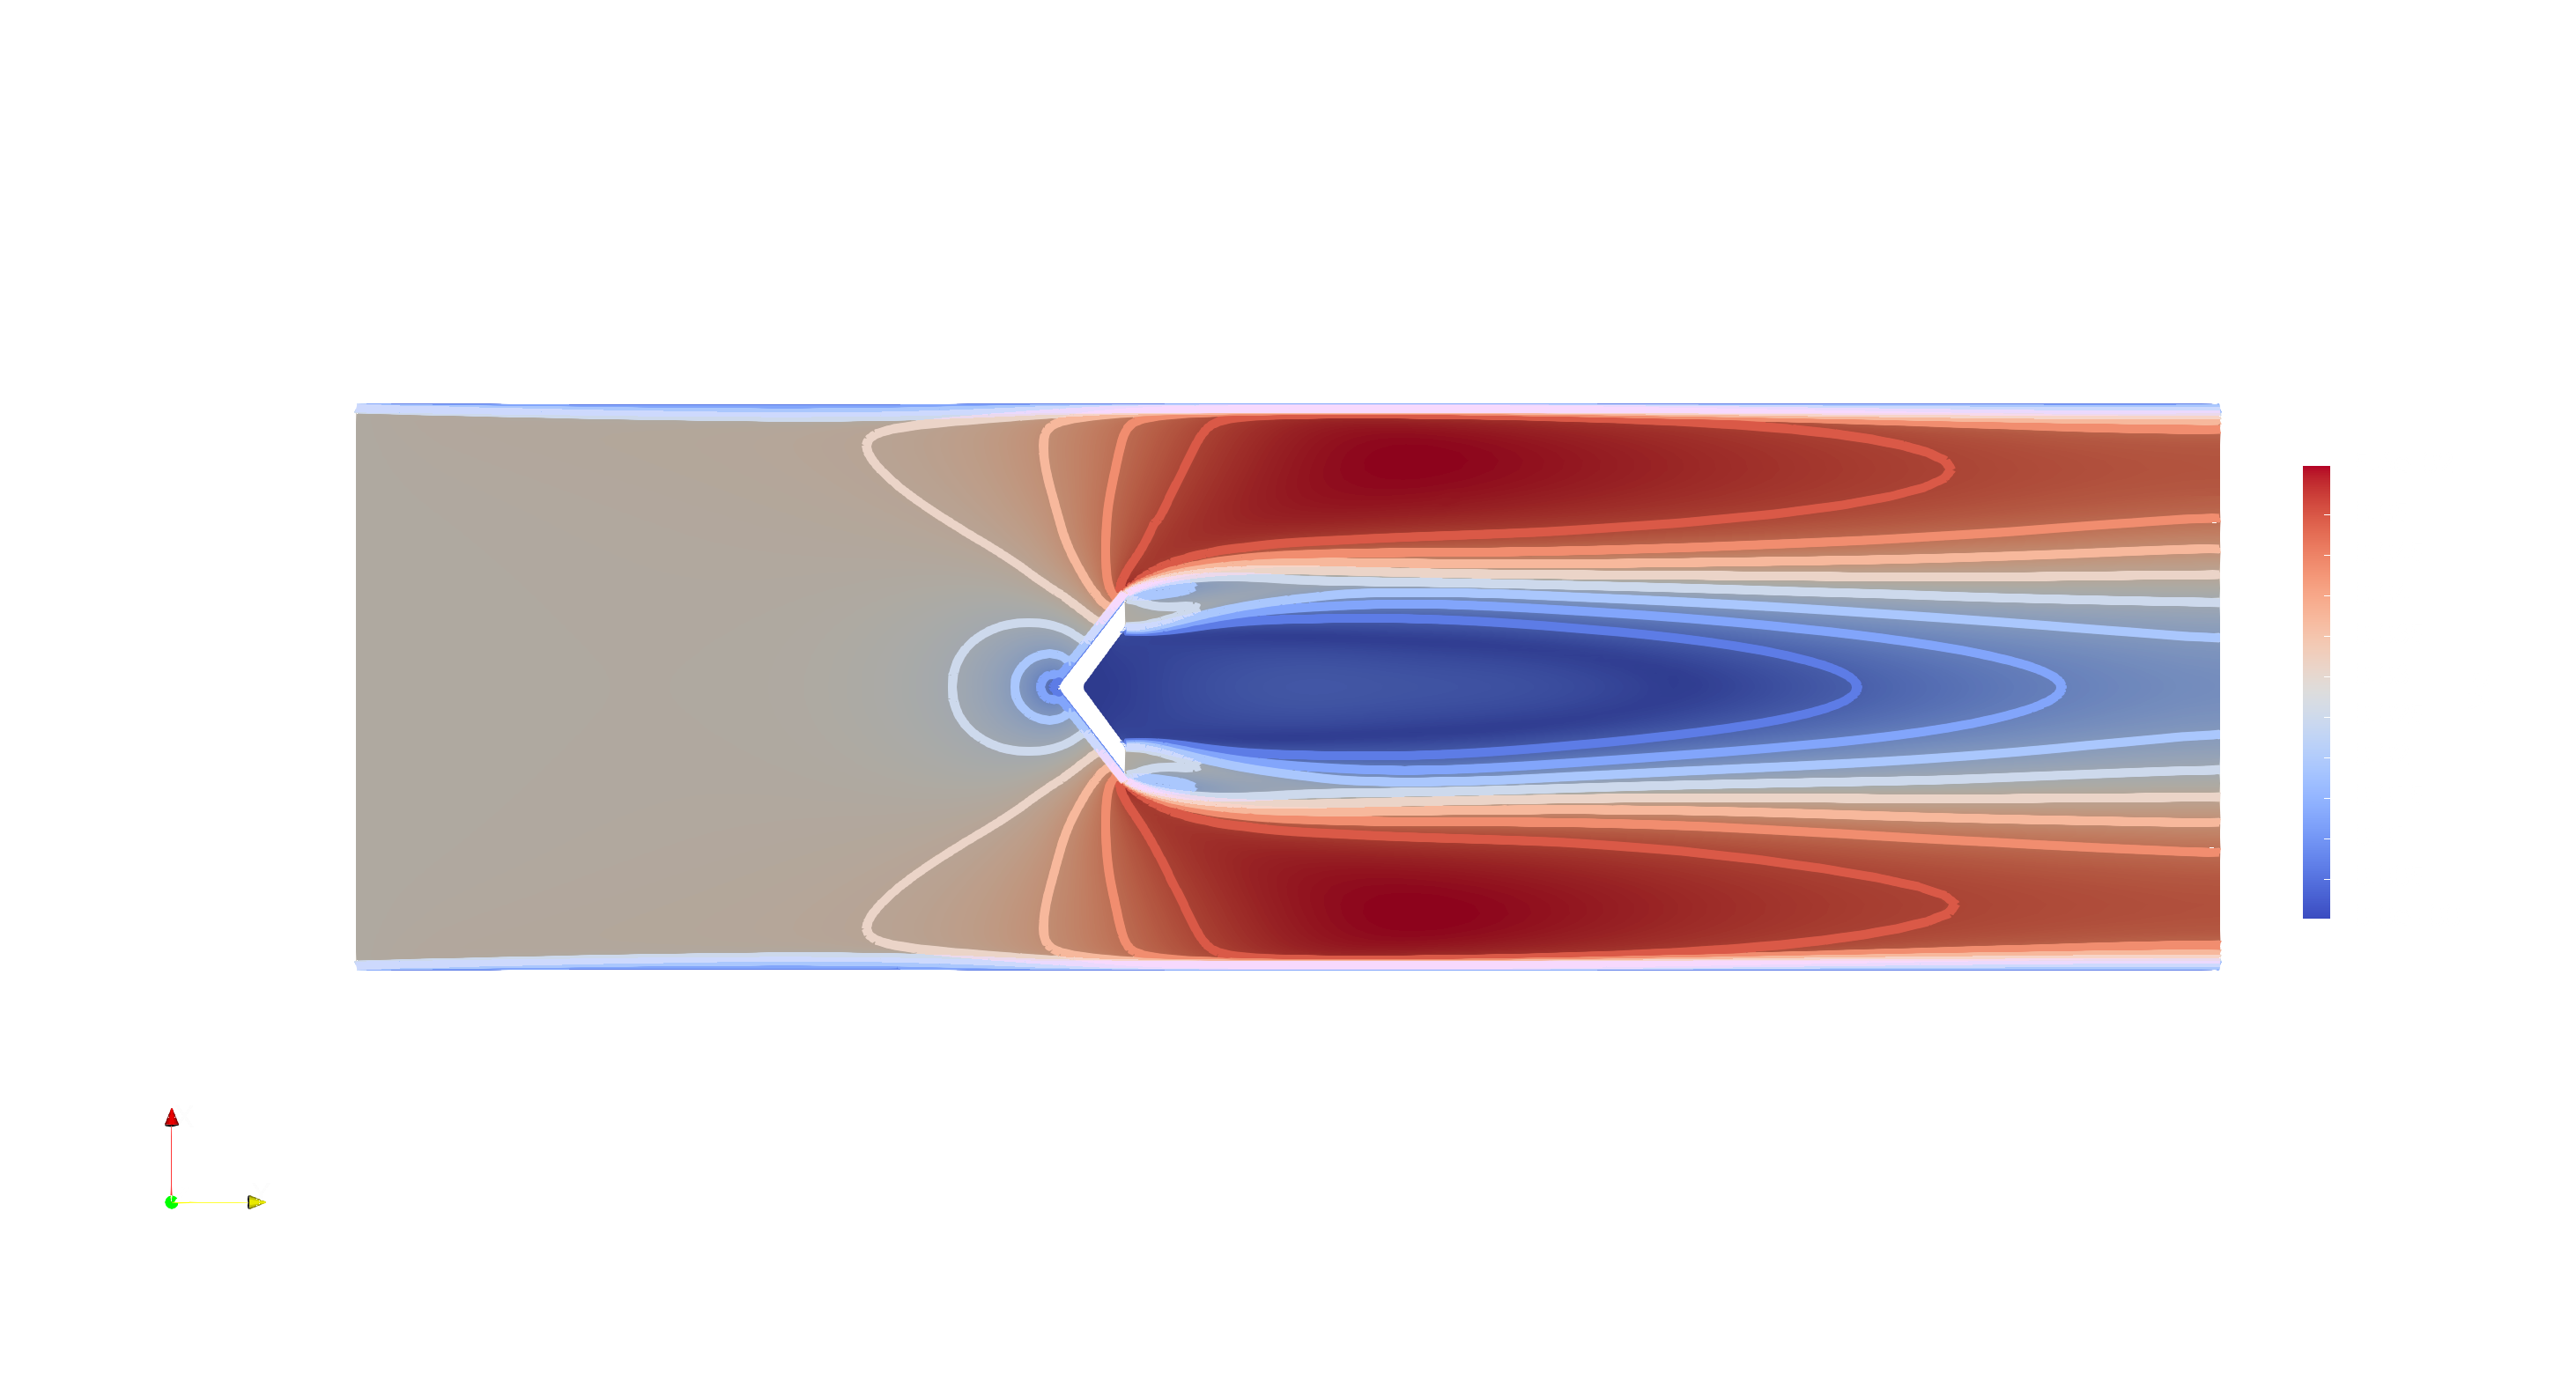
\includegraphics[width=\textwidth]{latexFIGS/figs/combustorMachHL.png}
    \cprotect\caption{Mach isolines for \verb|combustorRhoPimple_highT_lowRe| at $t = 0.4s$.}
\end{figure}

\begin{figure}[!h]
    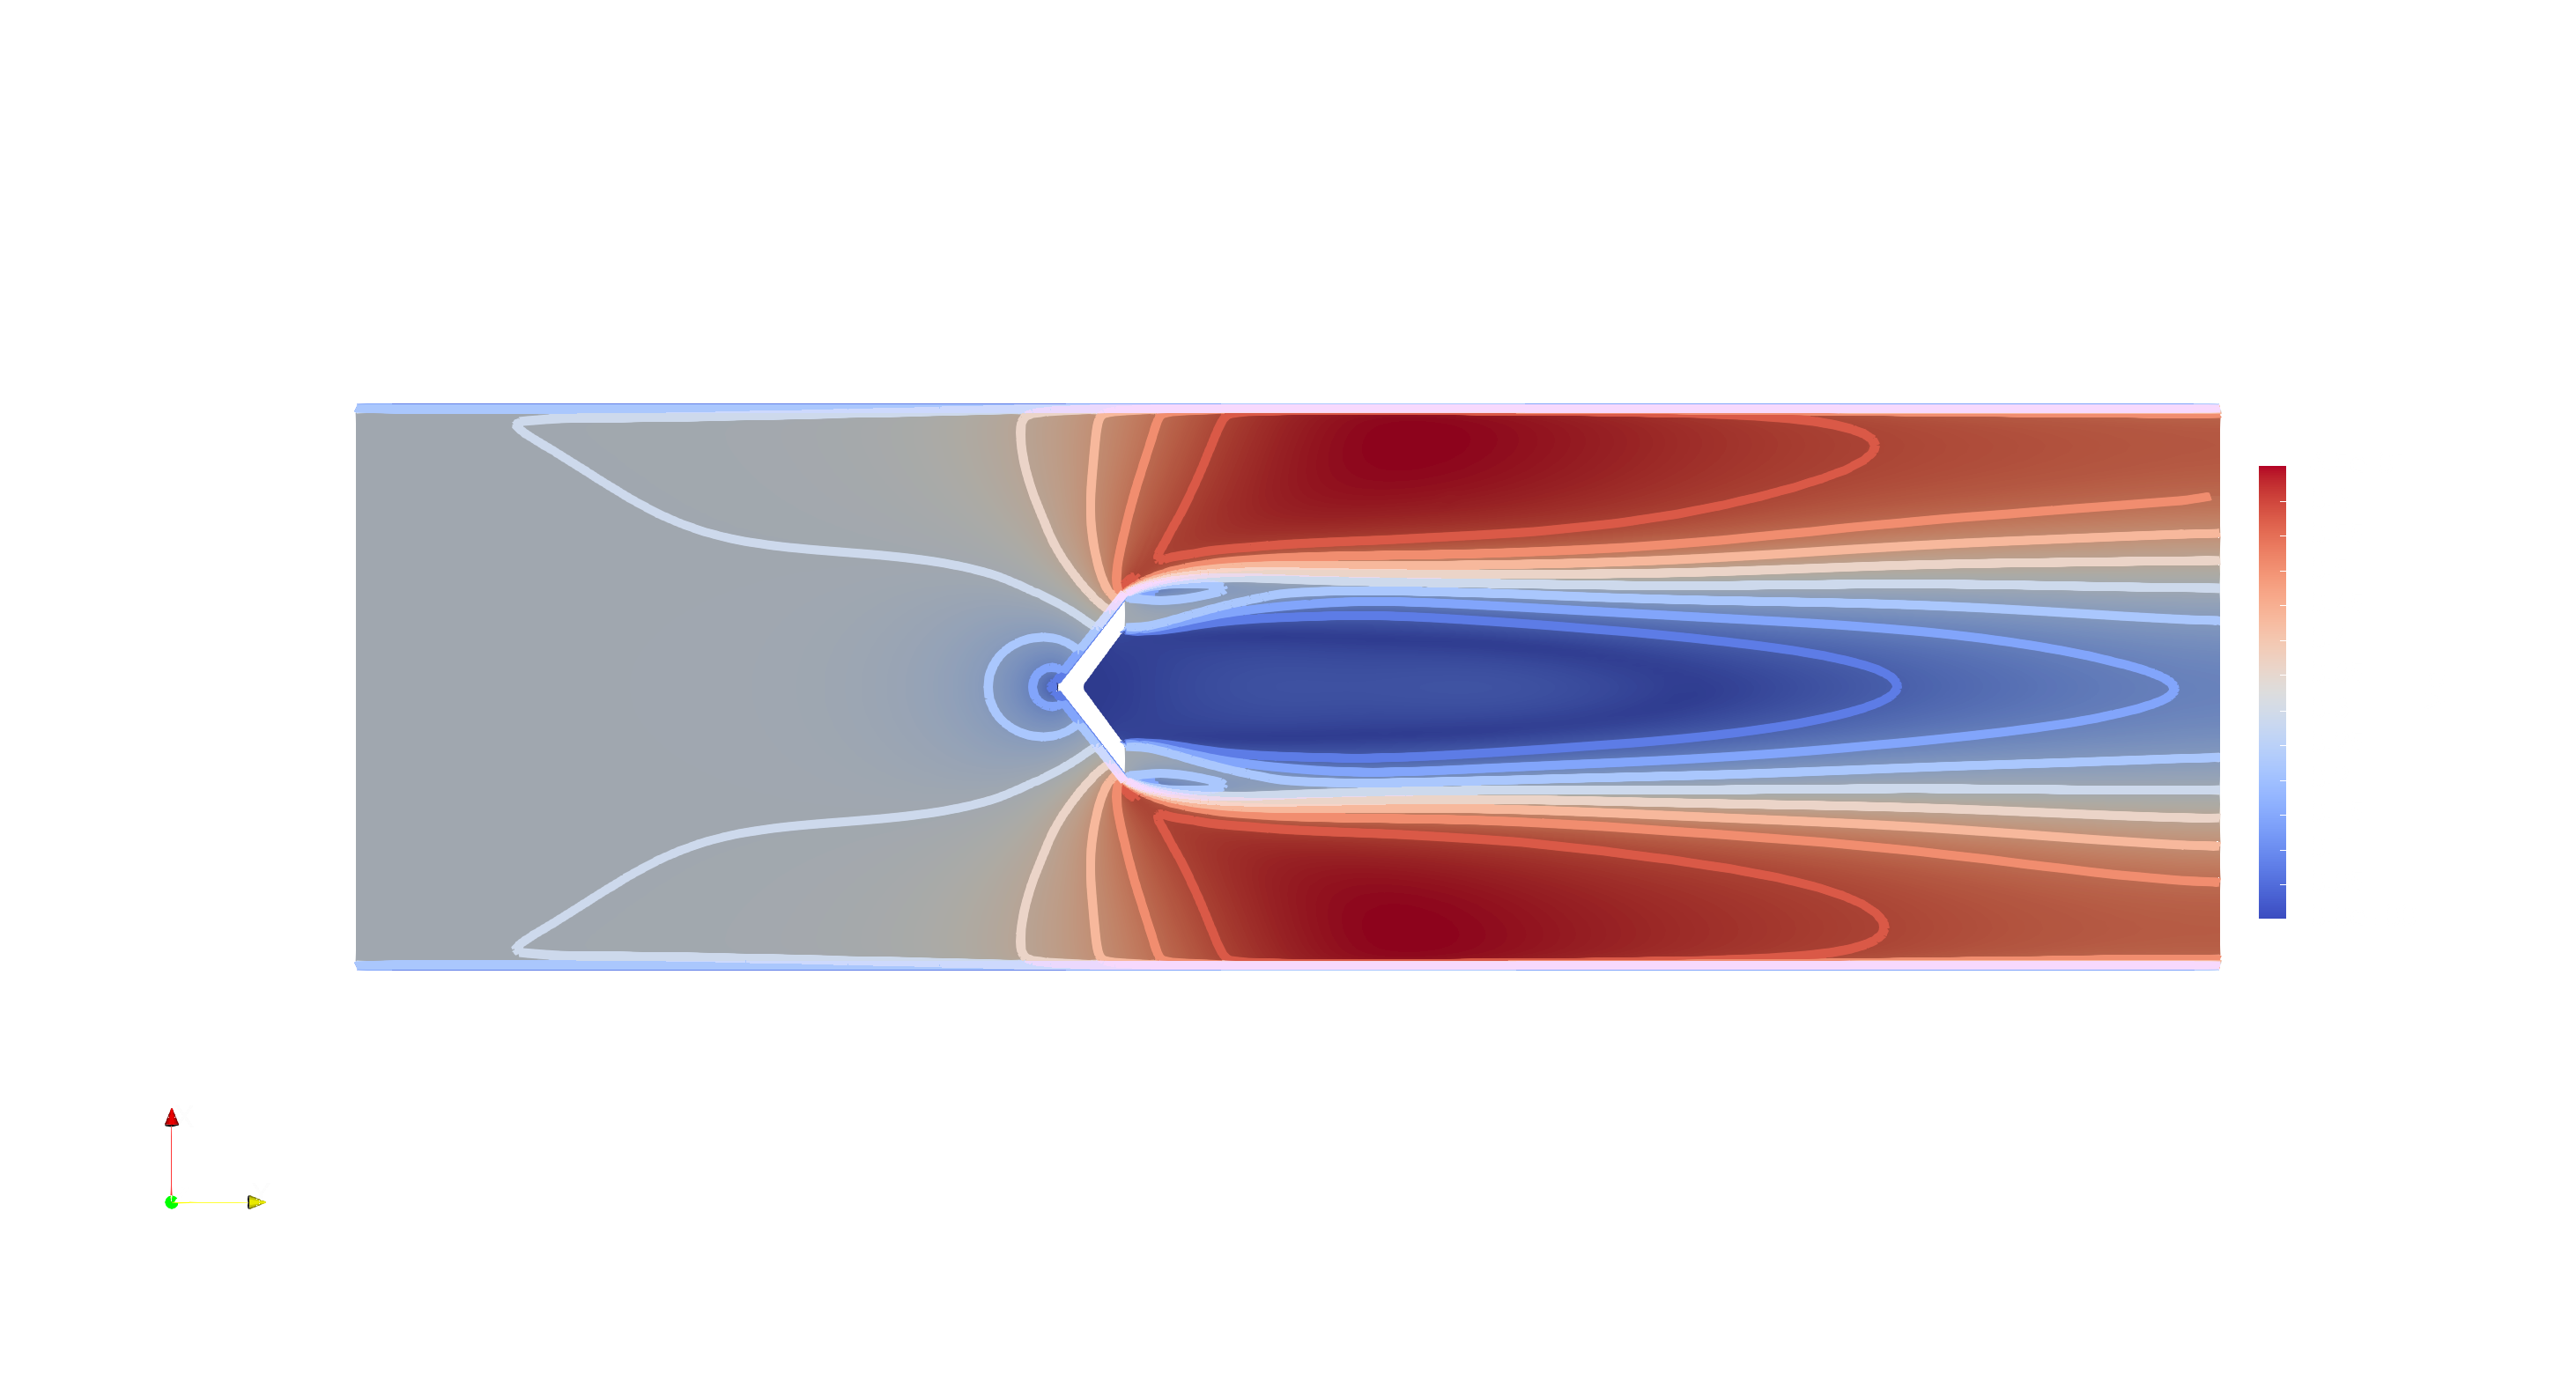
\includegraphics[width=\textwidth]{latexFIGS/figs/combustorMachHH.png}
    \cprotect\caption{Mach isolines for \verb|combustorRhoPimple_highT_highRe| at $t = 0.4s$.}
\end{figure}

\clearpage

    \newpage
    % !TEX root = ~/OpenFOAM/antoniopucciarelli-9/run/LABS/thermochemical_CFD/main.tex

\section{Lagrangian particles tracking and wall-film modeling - $\mathtt{Lab05}$ and $\mathtt{Lab06}$}
    
    \renewcommand{\thepage}{\arabic{page}}
    \setcounter{page}{\thelastPage}
Spray modeling and wall-film theory are described in appendix~\ref{app:app3_1} and appendix~\ref{app:app3_2}.    
%    \subsection{Spray modeling}
%    \subsubsection{Spray description and lagrangian particles approach}
%    Sprays are largely used in the combustion field. The aim is to let the fuel evaporate in the shortest time possible to reach the best performances.
%    Engineers have divided the spray in 3 regions and one of the main describers can be the void fraction\footnote{$\alpha = \frac{V_{liquid}}{V_{cell}}$}: 
%    \begin{itemize}
%        \item \textbf{Dense region} In this region, there is the first break up of the jet core in many string shaped drops. The fuel has a low surface to volume ratio, this implies the fuel is a dense and confined region in the system. This region has to be treated with care and it is very computationally demanding. The models required to solve this region are called \textbf{continuous phase models}, \verb|CPM|. The void fraction for this region is around unity. 
       
%        \item \textbf{Diluted region} In this region, the dense region starts to break up into smaller pieces; these pieces have a larger surface to volume ratio but not high enough to be modelled as spheric particles. This region is very important to lagrangian particles tracking methods because it is the region of transition between dense to dispersed region. This region can be treated as well with \verb|CPM|. The final aim of the \verb|CPM| in this case is to get a good description of the spray properties for the dispersed region modeling. The void fraction is around $0.5$ - this because $\frac{V_{liquid}}{V_{gas}} \approx 1$.
        
%        \item \textbf{Dispersed region} This region consists of many dispersed particles where the surface to volume ratio is high enough to consider these particles as spheres. This \textbf{huge} simplification allows using the lagragian spray method for the modeling of the development of the spray in the dispersed region\cprotect\footnote{It is possible to model the dispersed region with \verb|CPM|. Using \verb|CPM| in the dispersed region means not considering the particles as spheres. \verb|CPM| in dispersed region is very computational demanding and very difficult to handle.}. In the following CFD cases, lagrangian particles models are used to discretize the spray evolution (dispersed region only) into the system. As result of dispersed fuel into the system, the void fraction is lower than $1$.
%    \end{itemize}

%    \subsubsection{Parcels in spray modeling}
%    The number of particles in the dispersed region can be of order of billions; this will bring a lot of computational effort to model all the particles into the system and also to store all the data related to particles' properties, position and dynamics. In order to solve this problem, lagrangian sprays adopted a new way of modeling for these particles.
%    All these particles are grouped into objects called parcels. The grouping process is related to the particles' diameter. If a particle has a certain diameter, this particle will be grouped with other particles that fall inside a defined diameter range. Particles' diameter is defined by experimental results, by results analysis of dense and diluted region simulations and by statistics. After the grouping process, every parcel in the system has defined properties. The lagrangian spray modeling will compute the parcels evolution into the system. 
    
%    \paragraph{Parcels interaction}
%    Since parcels represent the properties of group of particles, the evolution of parcels represents the evolution of those particles. Parcels and gaseous flow can interact in different ways. This depends on the nature of the spray, on parcels' properties and on computational power available. It is possible to model the spray as:
%    \begin{itemize}
%        \item \textbf{One way coupling} The one way coupling allows only a \textit{one way talk} from the continous phase to the discrete phase. This allows to compute the parcels motion directly from the continuous phase field. Of course, parcel motion depends on the forces applied to it; these forces are computed using forces equations applied to spherical shaped particels with the help of experimental results. The forces' models depend on particles diameter - expressed through parcel object -, the particles diameter on the other hand depends on the thermodynamics (because of evaporation).
%        \item \textbf{Two ways coupling} The two way coupling allows the \textit{talk back} of the discrete phase evolution to the continous phase. This happens through additional source terms in the continuous phase equations. As result, this method is more computational demanding\footnote{All the modeling aspects for the parcel's evolution are the same as the one way coupling}.
%        \item \textbf{Four ways coupling} The four ways coupling accounts also to the parcels interaction. Usually this method is used when $\alpha \geq 10^{-2}$. The continuous phase treatment remains almost the same as the two ways coupling but the parcels interaction has an additional modeling step that takes into account the changes parcels make into the continuous field because their distance and also the parcels interaction as parcels agglomeration and parcels break-up.
%    \end{itemize}

%    \subsection{Wall-film modeling}
%    The particles-wall interaction has to be treated by the simulation. This interaction is very important because it can change a lot the behaviour of the solution. Wall-film in OpenFOAM are mainly treated using these hypothesis:
%    \begin{itemize}
%        \item \textbf{Wall-film thickness hypthesis} The wall-will thickness is supposed to be very thin; this brings to study the liquid film evolution as a 2D problem
%        \item \textbf{Particles temperature change} The temperature change of the particles impinging the wall-film is slow; this allows direct analytical time integration istead of numerical integration
%        \item \textbf{Conductivity hypothesis} Since the wall-film region is a layer above the solid wall, heat is transmitted from the wall to the liquid film through conductive mechanism
%        \item \textbf{Temperature limits hypothesis} Due to modeling reasons, the wall and wall-film temerature is supposed to be lower than the liquid boiling temperature
%    \end{itemize}
%
%    \subsubsection{Mesh and boundary conditions}
%    Because the wall-film region can be seen as an additional model to the usual \verb|FVM| case, a mesh has to be built in order to study the wall-film region. The only purpose of the wall-film mesh is to track the development of a 3D wall-film using a 2D mesh. The wall-film has to talk back to the \textit{global} mesh in order to set up correct boundary conditions for the main flow. As result of this modeling choices, the main parameters that describe the wall-film region are:
%    \begin{itemize}
%        \item $\delta$ Liquid film height. Since the mesh is 2D, the wall film height is described by $\delta$ but at the same time $\delta$ describes the presence of the liquid film on the wall-film region surface
%        \item $\boldsymbol{u}$ Liquid film velocity
%        \item $T$ Liquid film temperature
%    \end{itemize}
%    
%    Transport equations~(\ref{eqn:transp}) are used for tracking these quantities:
%    \begin{equation}
%        \begin{cases}
%            \frac{\partial \rho \delta}{\partial t}  + \boldsymbol{\nabla} \cdot \big( \rho \ \delta \ \boldsymbol{u} \big) & = \boldsymbol{S}_{\delta} \\ 
%            \frac{\partial \rho \delta \boldsymbol{u} }{\partial t}  + \boldsymbol{\nabla} \cdot \big( \rho \ \delta \boldsymbol{u} \ \boldsymbol{u} \big) & = \boldsymbol{S}_{\delta \boldsymbol{u}} \\ 
%            \frac{\partial \rho \delta h }{\partial t}  + \boldsymbol{\nabla} \cdot \big( \rho \ \delta h \ \boldsymbol{u} \big) & = \boldsymbol{S}_{\delta h}
%        \end{cases} \label{eqn:transp}
%    \end{equation}

    \subsection{Problem setup}
    It is possible to see this new case as the previous compressible case plus two \textbf{additional layers} of modeling: the lagrangian particles evolution and the surface wall-film modeling. 
    These new layers are described by defined dictionaries. The \verb|fvModels| allows to enable these dictionaries and to \textbf{wrap} them into the \textit{main} case. The wall-film region is generated through the \verb|topoSet| dictionary. This dictionary coverts patch of the system into \verb|faceSet| or \verb|faceZoneSet| objects; these objects allow to make new operations such as wall-film region generation. The wall-film region is made using the \verb|extrudeToRegionMesh| dictionary. This dictionary makes a one layer 2D mesh from the patch converted by \verb|topoSet| firstly into \verb|faceSet| and then into \verb|faceZoneSet|. As additional step, it is necessary to change the boundary conditions; this means that the \textit{main} field and the wall-film region field (in \verb|0/wallFilmRegion|) have to set their boundary conditions on the \verb|faceZoneSet| generated\cprotect\footnote{This is done through the \verb|bash| script \verb|AllSplitterRegion|.}. 

    \cprotect\subsubsection{\verb|cloudProperties|}
    This dictionary is a describer of the injector properties. The injector properties are summed up in parcels number, velocity, temperature, distribution and timing. These properties are assigned in \verb|subModels -> injectionModels|. The force applied to the parcels are described in \verb|particleForces|; only drag forces are present. The distribution model used is the \verb|RosinRammler|. The interaction between parcel and wall is set as \verb|rebound| (particle bumps on the surface). Particles diameter is allowed to change with an evaporation model set as \verb|liquidEvaporationBoil|\cprotect\footnote{Every chemical property of the liquid is described in \verb|chemkin| folder and converted into OpenFOAM syntax with \verb|chemkinToFoam| command in \verb|bash|.}. \verb|breakupModel| describes the particle break up interaction into the simulation.   

    \cprotect\subsubsection{\verb|surfaceFilmProperties|}
    The liquid film modeling is described by a complicated dictionary that containts in itself many submodels. These submodels are describers of the interaction of the wall-film with the \textit{main} flow. \verb|viscosity|, \verb|momentumTransport|, \verb|forces| and \verb|ejection| are the main subdictionaries. The \verb|ejection| subdictionary describes the interaction of the liquid film with the splitter geometry with respect to its \textbf{shape}. 
    
    \subsection{Post-processing}
    The post-processing setup is different from the previous cases. There exist different ways to get the results. Using the python code \verb|latexData.py|, data from parcels size distribution and liquid penetration are available. A useful post-processing tool is \verb|foamToVTK|. This command allows to reconstruct the case and all its properties in \verb|VTK| format.

    \subsection{Result}
    The main differences between the different cases consist into particles breakup model - in \verb|cloudProperties| - and \textit{main} flow temperature. 
    
    \cprotect\subsubsection{\verb|combustorSprayWallFilmReitzKHRT|}
    This case uses the \verb|ReitzKHRT| breakup model. The effect of \verb|rebound| setting in \verb|cloudProperties| is very evident in the final solution. The particle jet reaches its maximum amplitude at the middle of the simulation due the the \verb|sine| flow rate setting. Most of the particles impinges on the splitter. There are particles that are still not fully evaporated after passed the splitter. 

    \cprotect\subsubsection{\verb|combustorSprayWallFilmReitzDiwakar|}
    This case uses the \verb|ReitzDiwakar| breakup model. The jet behaviour is similar to the \verb|ReitzKHRT|. There are changes in the particles distribution over time and of the liquid penetration. The reason relies in the way the breakup of the parcels is modeled; it is like the \verb|ReitzDiwakar| treats the particles as less interactive with the environment (this explains why the liquid jet penetration is a bit higher than \verb|ReitzKHRT|).

    \cprotect\subsubsection{\verb|combustorSprayWallFilmReitzKHRT450|}
    This last case uses the \verb|ReitzKHRT| breakup model and \verb|fixedValue -> value 450;| as boundary condition for the \verb|T| at the \verb|inlet|\cprotect\footnote{The other two cases used \verb|fixedValue -> value 300;| as inlet temperature boundary condition.}. The solution is completelly different from the previous ones. This because the higher temperature of the \textit{main} flow that allows faster evaporation of the parcels into the system.

    \newpage

    % PAGE MANAGEMENT 
    \setcounter{lastPage}{\thepage}
    \renewcommand{\thepage}{SWF-\roman{page}}
    \setcounter{page}{1}

    \begin{figure}[!ht]
        \centering
        \import{latexFIGS/lab0506/}{residuals.pgf}
        \caption{Surface \& wall-film cases: residuals.}
    \end{figure}

    \begin{figure}[!ht]
        \centering
        \import{latexFIGS/lab0506/}{phase95.pgf}
        \caption{Surface \& wall-film cases: liquid penetration.}
    \end{figure}

    \begin{figure}[!ht]
        \centering
        \import{latexFIGS/lab0506/}{diam.pgf}
        \caption{Surface \& wall-film cases: parcels diameter.}
    \end{figure}

    \begin{figure}[!ht]
        \centering
        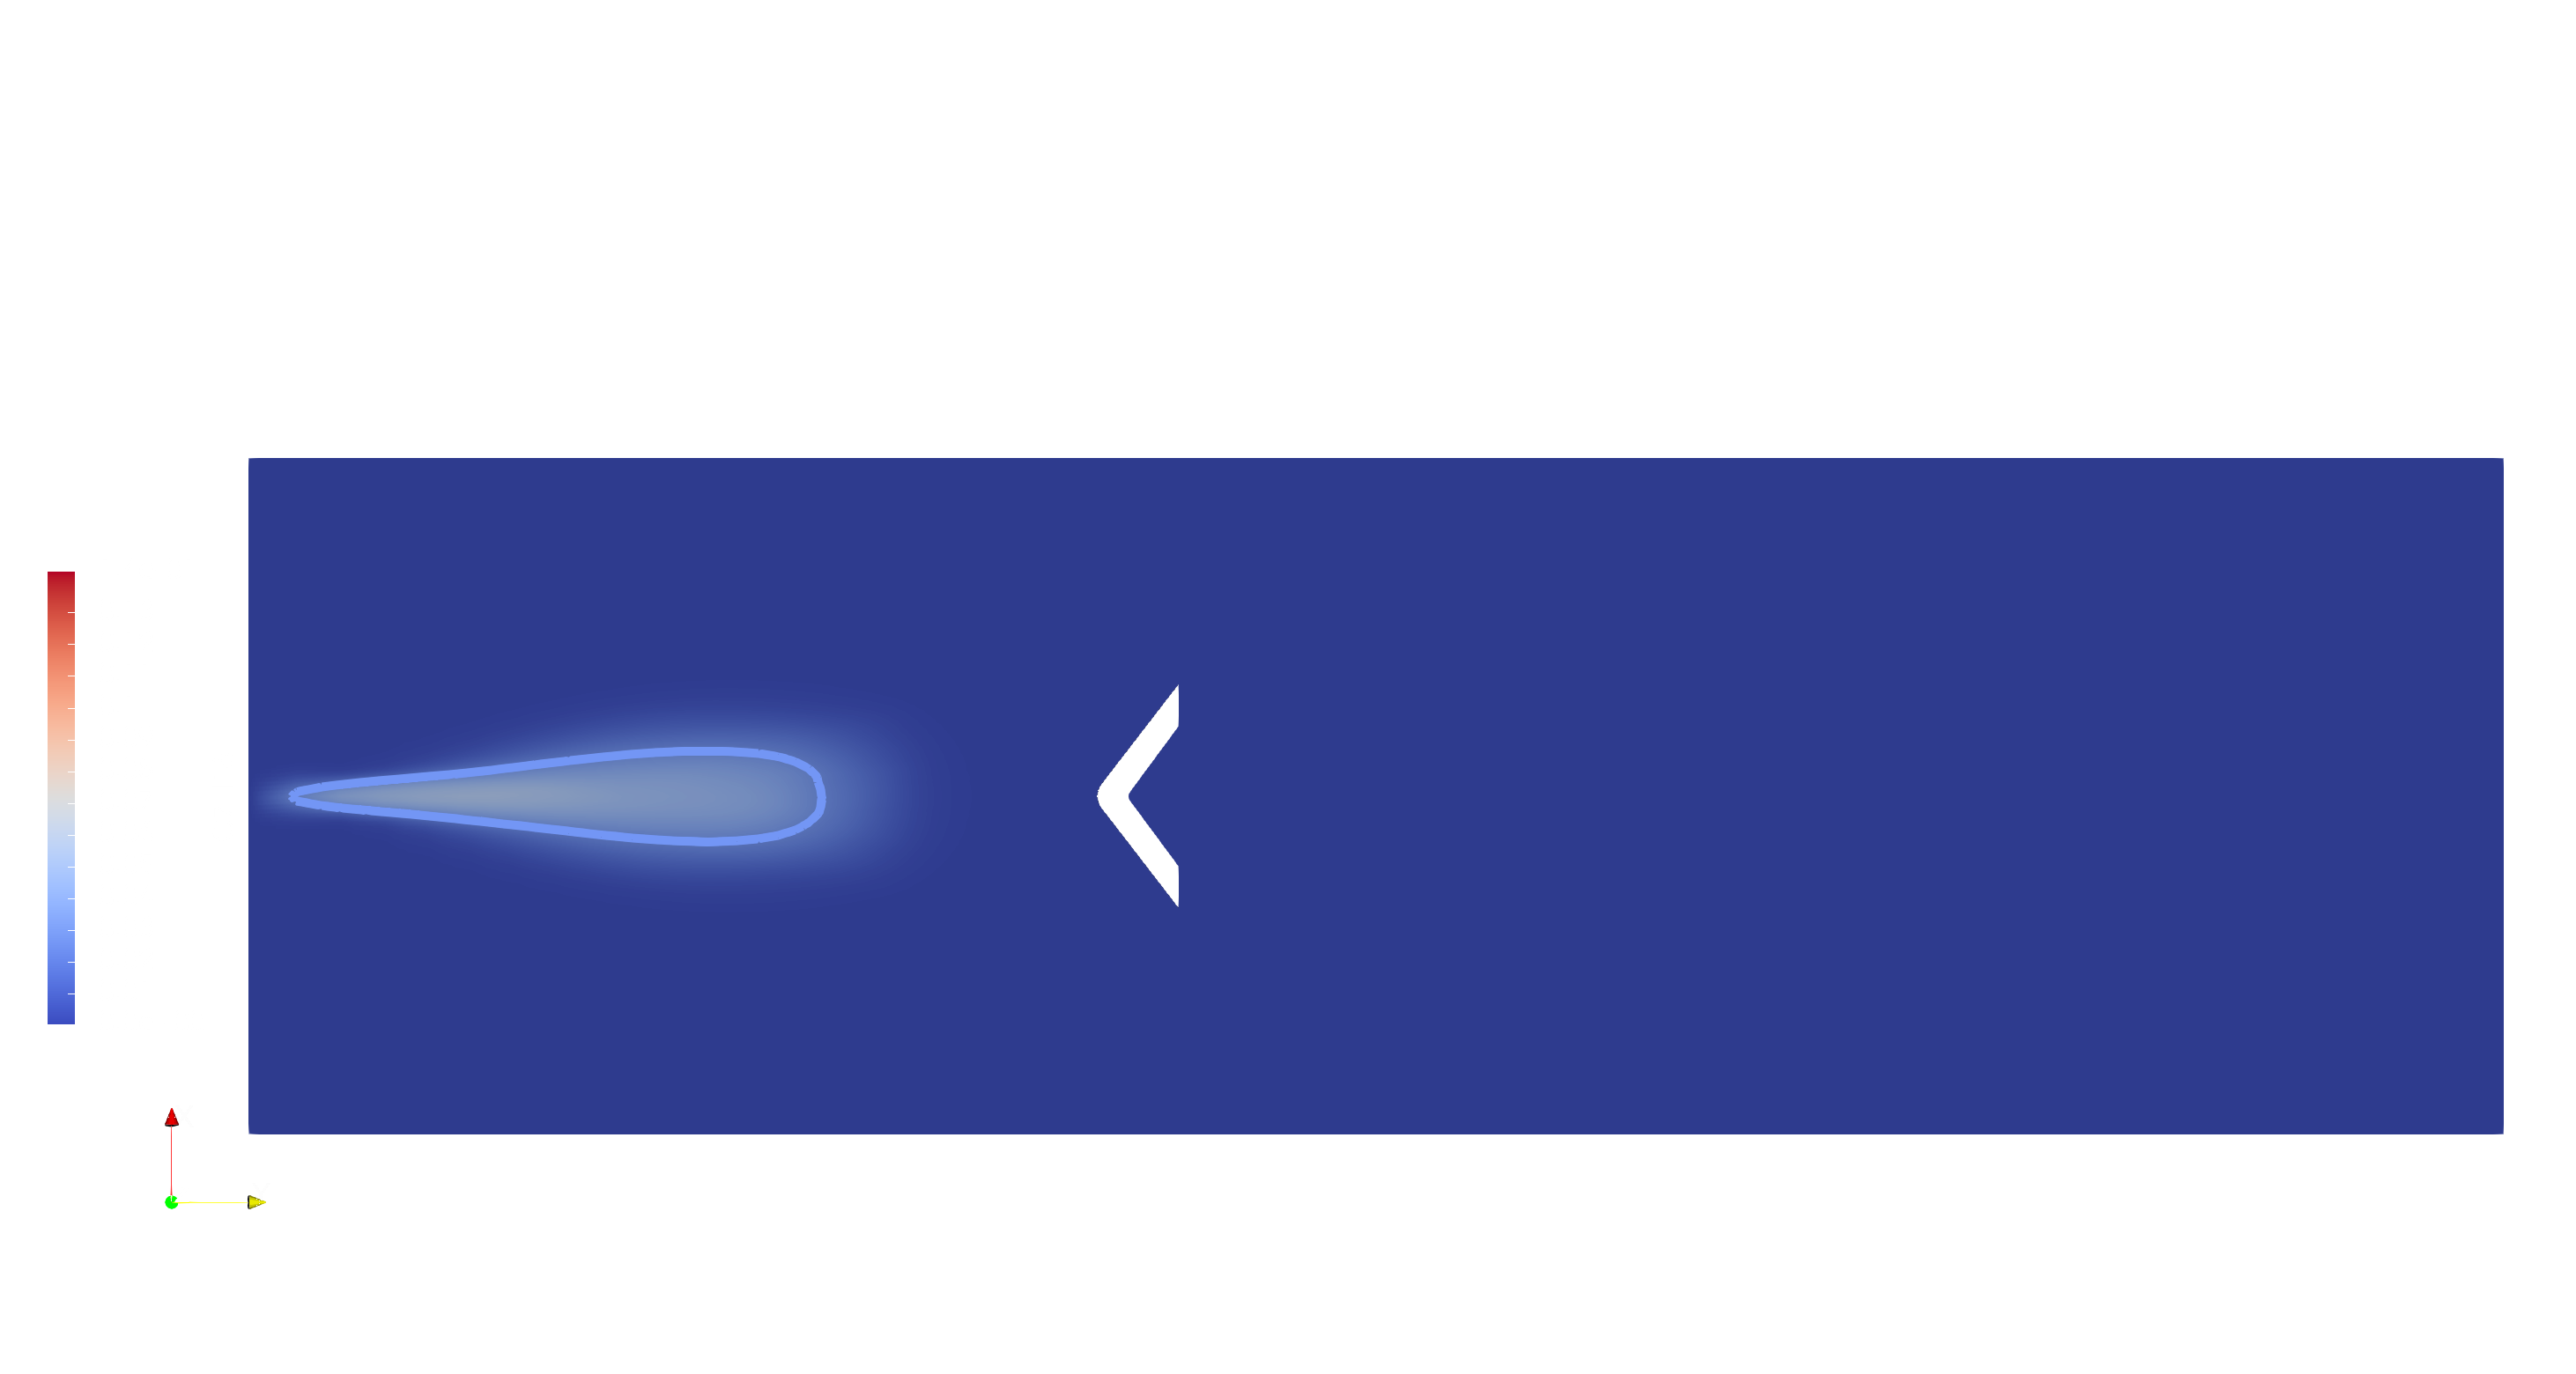
\includegraphics[height=0.25\textheight]{latexFIGS/figs/combustorC7H16_002.png}
        \cprotect\caption[\verb|C7H16| evaporation contour tracking, $t = 0.02s$.]{\verb|C7H16| evaporation contour tracking, $t = 0.02s$. \\ \verb|combustorSprayWallFilmReitzDiwakar|}
    \end{figure}
    
    \begin{figure}[!h]
        \centering
        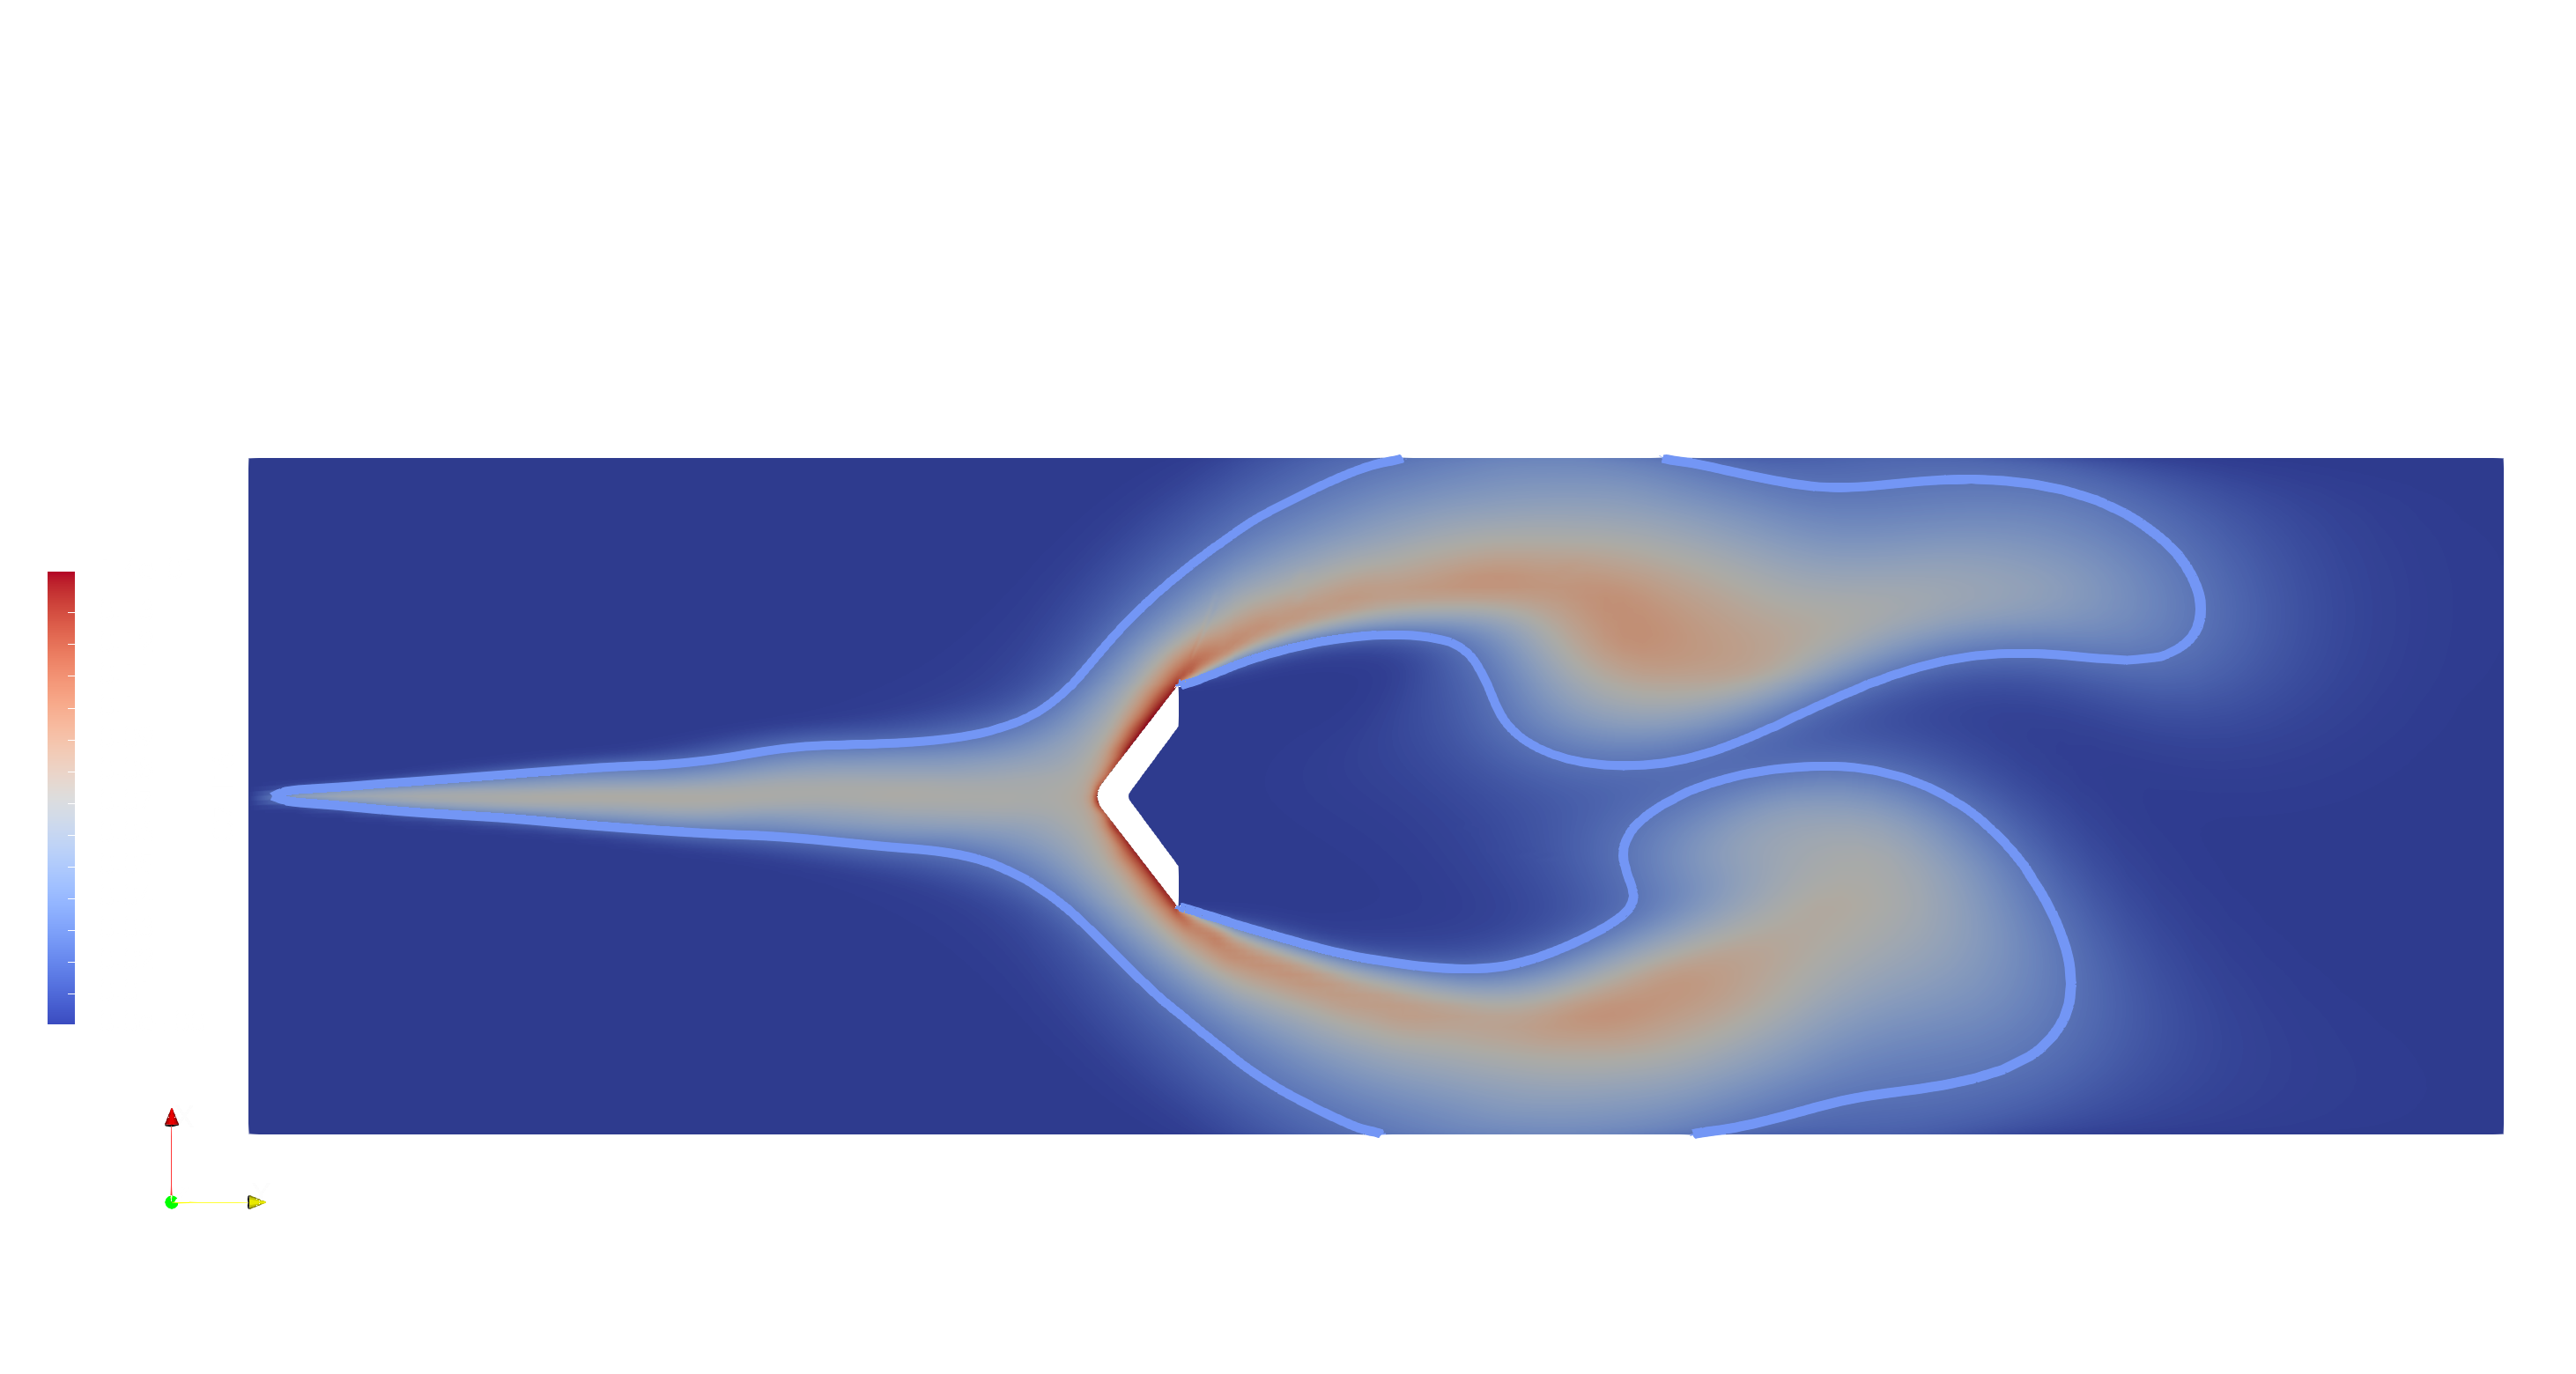
\includegraphics[height=0.25\textheight]{latexFIGS/figs/combustorC7H16_005.png}
        \cprotect\caption[\verb|C7H16| evaporation contour tracking, $t = 0.05s$.]{\verb|C7H16| evaporation contour tracking, $t = 0.05s$. \\ \verb|combustorSprayWallFilmReitzDiwakar|}
    \end{figure}
    
    \begin{figure}[!hb]
        \centering
        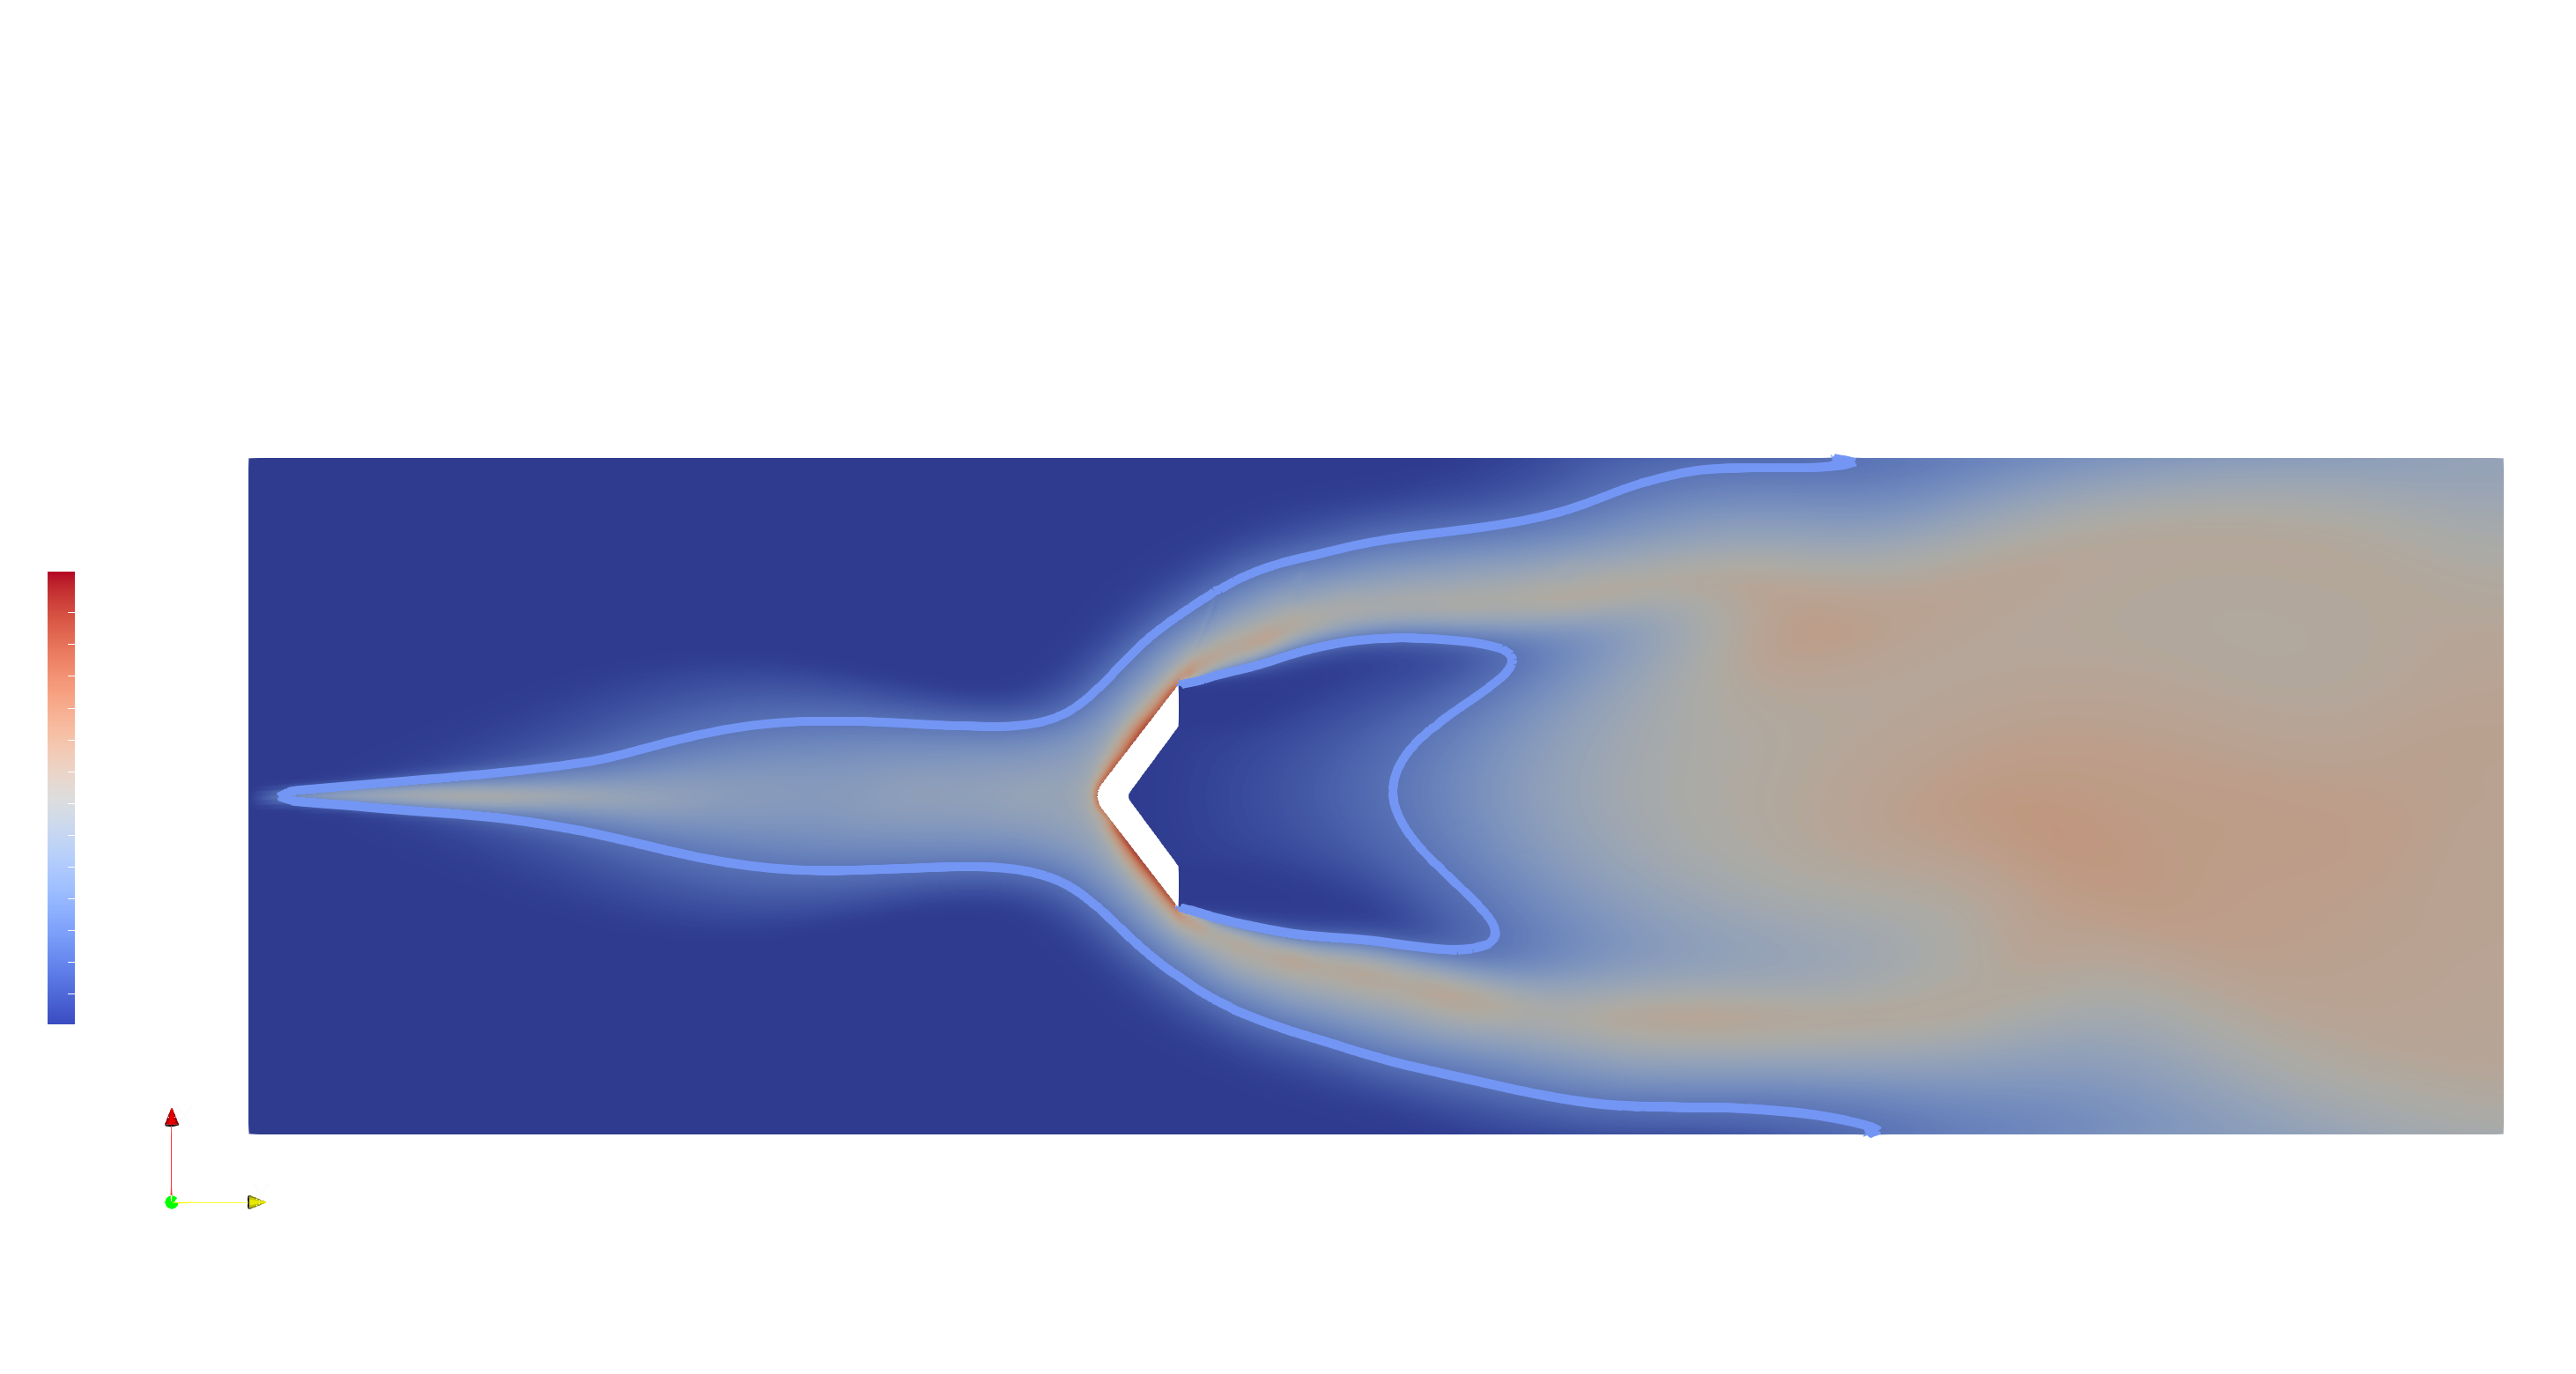
\includegraphics[height=0.25\textheight]{latexFIGS/figs/combustorC7H16_008.png}
        \cprotect\caption[\verb|C7H16| evaporation contour tracking, $t = 0.08s$.]{\verb|C7H16| evaporation contour tracking, $t = 0.08s$. \\ \verb|combustorSprayWallFilmReitzDiwakar|}
    \end{figure}

    \clearpage

    \newpage
    % !TEX root = ~/OpenFOAM/antoniopucciarelli-9/run/LABS/thermochemical_CFD/main.tex

\section{Reacting flows - $\mathtt{Lab07}$} \label{sec:lab07}
    
    \renewcommand{\thepage}{\arabic{page}}
    \setcounter{page}{\thelastPage}
    
    This section treats the numerical modeling of chemical reactions. Reactions are treated as well as the spray modeling and the wall-film surface modeling, they are seen as an \textbf{additional layer} to the \verb|FVM| problem. This additional modeling layer has to be blended into the \textit{main} flow solution as it happened with lagrangian spray modeling and wall-film modeling.
The important concepts related to combustion theory and modeling are explained in~\ref{app:app4}.
%    \subsection{Reactions}
%    Before starting modeling reactions it is necessary to know the species inside the system, the possible reactions that can happen and all the parameters related to transport and diffusion of these species into the system. All these properties are mainly taken from experiments or they come from chemistry modeling (for the more complicated species). 
    
%    \subsubsection{Govering equations}
%    The main changes in the governing equation are made on the continuity equation. The continuity equation expresses the conservation of mass in the system. Because the presence of reactions, it is needed to track the species' evolution in the system. The continuity equations for each species are written as:
%    \begin{equation}
%        \frac{\partial \rho Y_i}{\partial t} + \boldsymbol{\nabla} \cdot \big( \rho \boldsymbol{u} \ Y_i  \big) = \boldsymbol{\nabla} \cdot \big( \rho \boldsymbol{v}_i \ Y_i \big) + \dot\omega_i
%    \end{equation}
%    Where $Y_i$ is the mass fraction of \textit{ith} species, $\boldsymbol{v}_i$ is the \textit{ith} species diffusion velocity\footnote{$\sum_i \boldsymbol{\nabla} \cdot \big( \rho Y_i \boldsymbol{v}_i \big) = 0$, where $\boldsymbol{v}_i$ is the species velocity fluctuation, $\sum_i Y_i = 1$ and $\boldsymbol{\nabla} \cdot \big( \rho \boldsymbol{u} \big) = 0$. \newline $\sum_i \boldsymbol{\nabla} \cdot \big[ Y_i \rho \big(\boldsymbol{u} + \boldsymbol{v}_i \big) \big] = \sum_i \boldsymbol{\nabla} \cdot \big( Y_i \rho \boldsymbol{u} \big) + \sum_i \boldsymbol{\nabla} \cdot \big( Y_i \rho \boldsymbol{v}_i \big) = \boldsymbol{\nabla} \cdot \big( \rho \boldsymbol{u} \sum_i Y_i \big) + \sum_i \boldsymbol{\nabla} \cdot \big( Y_i \rho \boldsymbol{v}_i \big) = 0$.} and $\dot\omega_i$ is the \textit{ith} species production due to reactions\footnote{$\sum_i \dot\omega_i = 0$ because the reaction process does not create mass, it just \textit{moves} atoms in order to create new species, conserving mass.}. As result, $\boldsymbol{v}_i$ are new degree of freedom into the system, so it is necessary to find equations that allow to treat them. The complete equation for the $\boldsymbol{v}_i$ computation is very hard to solve\footnote{$\boldsymbol{v}_p$ equation: $\boldsymbol{\nabla}X_p = \sum_k \frac{X_p \ X_k}{\mathcal{D}_{p, k}}\big( \boldsymbol{v}_k - \boldsymbol{v}_p \big) + ( Y_p - Y_k \big) \frac{\boldsymbol{\nabla} p}{p} + \frac{\rho}{p} \ \sum_k Y_p \ Y_k \big( f_p - f_k \big)$.}, so it is necessary to simplify this equation. Possible formulations are the \textbf{Fick}'s law, equation~(\ref{eqn:fick}), and the \textbf{Hirshfelder}, equation~(\ref{eqn:hirsh}).
%        \begin{align}
%            \boldsymbol{v}_i & = - \mathcal{D} \boldsymbol{\nabla} \log{Y_p} \label{eqn:fick} \\ 
%            \boldsymbol{v}_i \ X_k & = \mathcal{D}_k \boldsymbol{\nabla} X_k \label{eqn:hirsh}  
%        \end{align}
%   All these simplified submodels imply a cost, mass conservation is not guaranteed. In order to conserve the mass, it is necessary to correct these fields through:
%   \begin{itemize}
%       \item Reducing the number of equations for the species from $N$ to $N-1$ using the mass conservation formula $\sum_i Y_i = 1$ for the computation of the \textit{Nth} species. This procedure can work but only if the $Y_N$ is high enough to neglect these modeling errors. 
%       \item A much better solution can be achieved changing the fluctuation field $\boldsymbol{v}_k$ in order to conserve total mass for all the species.
%   \end{itemize}

%    For the remaining governing equations, the main changes are relative the new source terms in the energy equation\footnote{The source term sign depends on the nature of the reaction.}. The momentum equation is affected most through the $\nu_{eff} = \nu + \nu_t$ due the dependence of viscosity and turbulence characteristics on the flow composition. 

%    \subsubsection{Chemistry}
%    Having introduced the way reactions talk with the \textit{main} flow governing equations, it is necessary to study the chemistry modeling in the system. This part is essential because it allows studing:
%    \begin{itemize}
%        \item \textbf{Combustion presence} If the energy activation threshold is overcomed, reaction takes place.
%        \item \textbf{Chemical kinetics} Allows to treat the species evolution - $\dot\omega_i$ in mass conservation equation -, control volume cell species composition - for $\nu_{eff}$ assembly in momentum equation.
%        \item \textbf{Chemical thermodynamics} Allows to treat heat transfered, $h_{reac}$, in energy equation. 
%    \end{itemize}
    
%    Most of the chemistry models are based on the \textbf{Arrhenius} law:
%    \begin{equation}
%        k = B \ T_a \ e^{- \frac{E_a}{R_u \ T}} \label{eqn:arrh}
%    \end{equation}

%    The equation~(\ref{eqn:arrh}) is a semi-empirical law\footnote{$B$ is the Boltzman constant, $B \ T_a$ is the collision frequency and $E_a$ is the energy activation for the reaction.} and it is used to determine the chemical kinetics of a reaction like the following:
    
%    \begin{equation}
%        \frac{\partial [C]}{\partial t} = (k_{forward} - k_{backward})  \ [A] \ [B]; \text{\ for the reaction}\footnote{The probability of having a reaction made by the interaction of more than three species is extremelly low.} \ A + B \leftrightarrow C \label{eqn:chemKin}
%    \end{equation}

%    Equation~(\ref{eqn:chemKin}) is an ODE that can be solved in an implicit or explicit way. Due to stiffness of equation (\ref{eqn:chemKin}) - related to the exponential nature of $k$ - an implicit formulation allows using less timesteps to reach the \textit{main} flow time step lenght but at the same time it is more computationally expensive. On the other hand, the explicit formulation in much more direct that the implicit one but it needs more iterative steps to reach the \textit{main} flow iterative time step lenght. 
    
%    As result, chemistry can be seen as a computational burden for the simulation because it is related to small time steps due to the chemistry ODE stiffness properties.

    \subsection{Problem setup}
    \subsubsection{Boundary conditions}
    Because the presence of different species - described by $Y_i$ -, it is necessary to know the control volume species composition at time $t = 0$. As result of this, species dictionaries are created as many as the species in the system\cprotect\footnote{\verb|Ydefault| dictionary can be found if the number of dictionaries does not match the number of species defined in the \verb|reaction| dictionary. \verb|Ydefault| dictionary is used only at $t = 0$, this because as the time step increases new species field are generated automatically by OpenFOAM.}. Since this simulation treats the combustion of \verb|CH4| with air, the fields dictionary set are \verb|CH4|, \verb|O2|, \verb|H2O|, \verb|N2| and \verb|CO2|. The initial values for the \verb|O2| and \verb|N2| field are computed from a previous simulation and then \textbf{mapped} into the \verb|combustorReaction| case. The new main property in the boundary conditions setup is the \verb|inletOutlet| type. This condition allows treating the field in a different manner with respect to inflow or outflow at the \verb|outlet| boundary\cprotect\footnote{At $t = 0$ the field takes the \verb|value| parameters, then it switches the cell center value with respect to the flow field direction at the outlet; if there is an inflow, the cell center takes $0$ value.}.

    \cprotect\subsubsection{\verb|chemistryProperties|}
    This dictionary describes the way chemistry is solved. Chemistry is activated through \verb|chemistry on;| and it is used an implicit method to solve it:
    \begin{lstlisting}[caption = $\mathtt{combustorReaction/constant/chemistryProperties}$ implicit chemistry model setup., label = list:chemProp]
        chemistryType
        {
            solver          EulerImplicit;
            chemistryThermo psi;
        }

        chemistry               on;

        initialChemicalTimeStep 1e-08;
    \end{lstlisting}
    
    The ODE implicit solver uses \verb|seulex|\cprotect\footnote{\verb|seulex| is an extrapolation-algorithm, based on the linearly implicit Euler method with step size control and order selection~\cite{wanner1996solving}. This method increases convergence order of an implicit method; this can be achieved using two different time steps and a control parameter.} solver and the initial time step for the chemistry solver is set at \verb|1e-08|. 
    \cprotect\subsubsection{\verb|combustionProperties|} \label{sec:PaSR}
    In this dictionary there are set information regarding how to treat the combustion as \textbf{laminar} flow or as \textbf{partial stirred reactor}. These two options are very important because they allow the \textit{talk} between the combustion model and the turbulence model (in this case \verb|RAS -> kEpsilon|). The \verb|PaSR| modeling allows using a much rapid dispersion of the species into the system, this due to the turbulence model relation\cprotect\footnote{Turbulence is expressed with $\nu_t$ in momentum equation diffusion term, the greater the turbulence the shorter the diffusion time. This concept affects also \verb|PaSR| combustion modeling.}. The \verb|laminar| setting is most used for supersonic combustion\footnote{This because turbulence diffusion has a longer characteristic time than that of the \textit{main} flow.} and for laminar flames\footnote{This because the turbulence is not present in the system and allows to have better and faster solutions.}.
    
    \cprotect\subsubsection{\verb|speciesThermo|} \label{sec:speciesThermo}
    This dictionary containts the information of all the species in the system. Every species is described with the atomic composition (name and number), molecular weight, transport properties and thermodynamics. Thermodynamic properties are described with temperature range in which thermodynamic properties \textbf{fit best} and the coefficients that are used to generate a polynomial fitting of the thermodynamic properties with respect to temperature.

    \cprotect\subsubsection{\verb|reactions|}
    This dictionary cointaints the rules to follow for the reaction modeling. In this case the reaction is just \textit{one way} and it is expressed with \verb|irreversibleArrheniusReaction|. There are expressed the reaction formula and all the needed parameters for describing Arrhenius law, equation~(\ref{eqn:arrh}).  

    \cprotect\subsubsection{\verb|thermophysicalProperties|}
    This dictionary is present for all the compressible flows. In order to make it work for the combustion simulation, it is necessary to link the thermodynamics of the species to this dictionary. These changes are in \verb|thermo|, \verb|mixture| and \verb|transport|. The inert specie \verb|N2| is declared as inert with \verb|intertSpecie N2;| command. 
    \begin{lstlisting}[caption = $\mathtt{combustorReaction/constant/thermophysicalProperties}$. This is the main link between the combustion model and the momentum transport equation., label = list:thermoProp]
        thermoType
        {
            type            hePsiThermo;
            mixture         multiComponentMixture;
            transport       sutherland;
            thermo          janaf;
            energy          sensibleEnthalpy;
            equationOfState perfectGas;
            specie          specie;
        }
    \end{lstlisting}
    All the data \verb|janaf| and \verb|sutherland| use are taken from \verb|thermo.mixture|\cprotect\footnote{That is essentially a copy of \verb|speciesThermo|.}.

    \subsection{Results}
    \cprotect\subsubsection{\verb|combustorRhoPimple|}
    This is just the initialization of the flow. The main purpose of this case is to setup a developed flow in order to avoid the establishing of the flow in the \verb|combustorReaction| case that would have been much more computationally demanding because the presence of combustion.

    \cprotect\subsubsection{\verb|combustorReaction|}
    The results show that there is a first mixing of \verb|CH4| with the surrounding air. At a determined point combustion happens due to close to stoichiometric conditions of the mixture. Once the flame is generated, the combustion propagates much faster and the generation of \verb|CO2| is much more evident than previously the flame generation\cprotect\footnote{If \verb|CH4| and air go in contact with proper temperature and pressure, reactoin happens but the heat generated from this reaction is related to the oxidizer-fuel ratio, \verb|OF|, of the mixture. A proof of this is the presence of \verb|CO2| before the flame develops.}. Simulation results show huge fluctuations on the residuals, this may be related to the presence of combustion. A check has been made in the \verb|log.reactingFoam| and no errors have been found.

    \newpage

    % PAGE MANAGEMENT
    % saving page number
    \setcounter{lastPage}{\thepage}
    % changing page numbering for the results figures
    \setcounter{page}{1}
    \renewcommand{\thepage}{REA-\roman{page}}

    \begin{figure}[!h]
        \centering
        \import{latexFIGS/lab07/}{residuals.pgf}
        \cprotect\caption{\verb|rhoPimpleFoam| case and \verb|reactingFoam| case: residuals.}
    \end{figure}
    
    \begin{figure}[!ht]
        \centering
        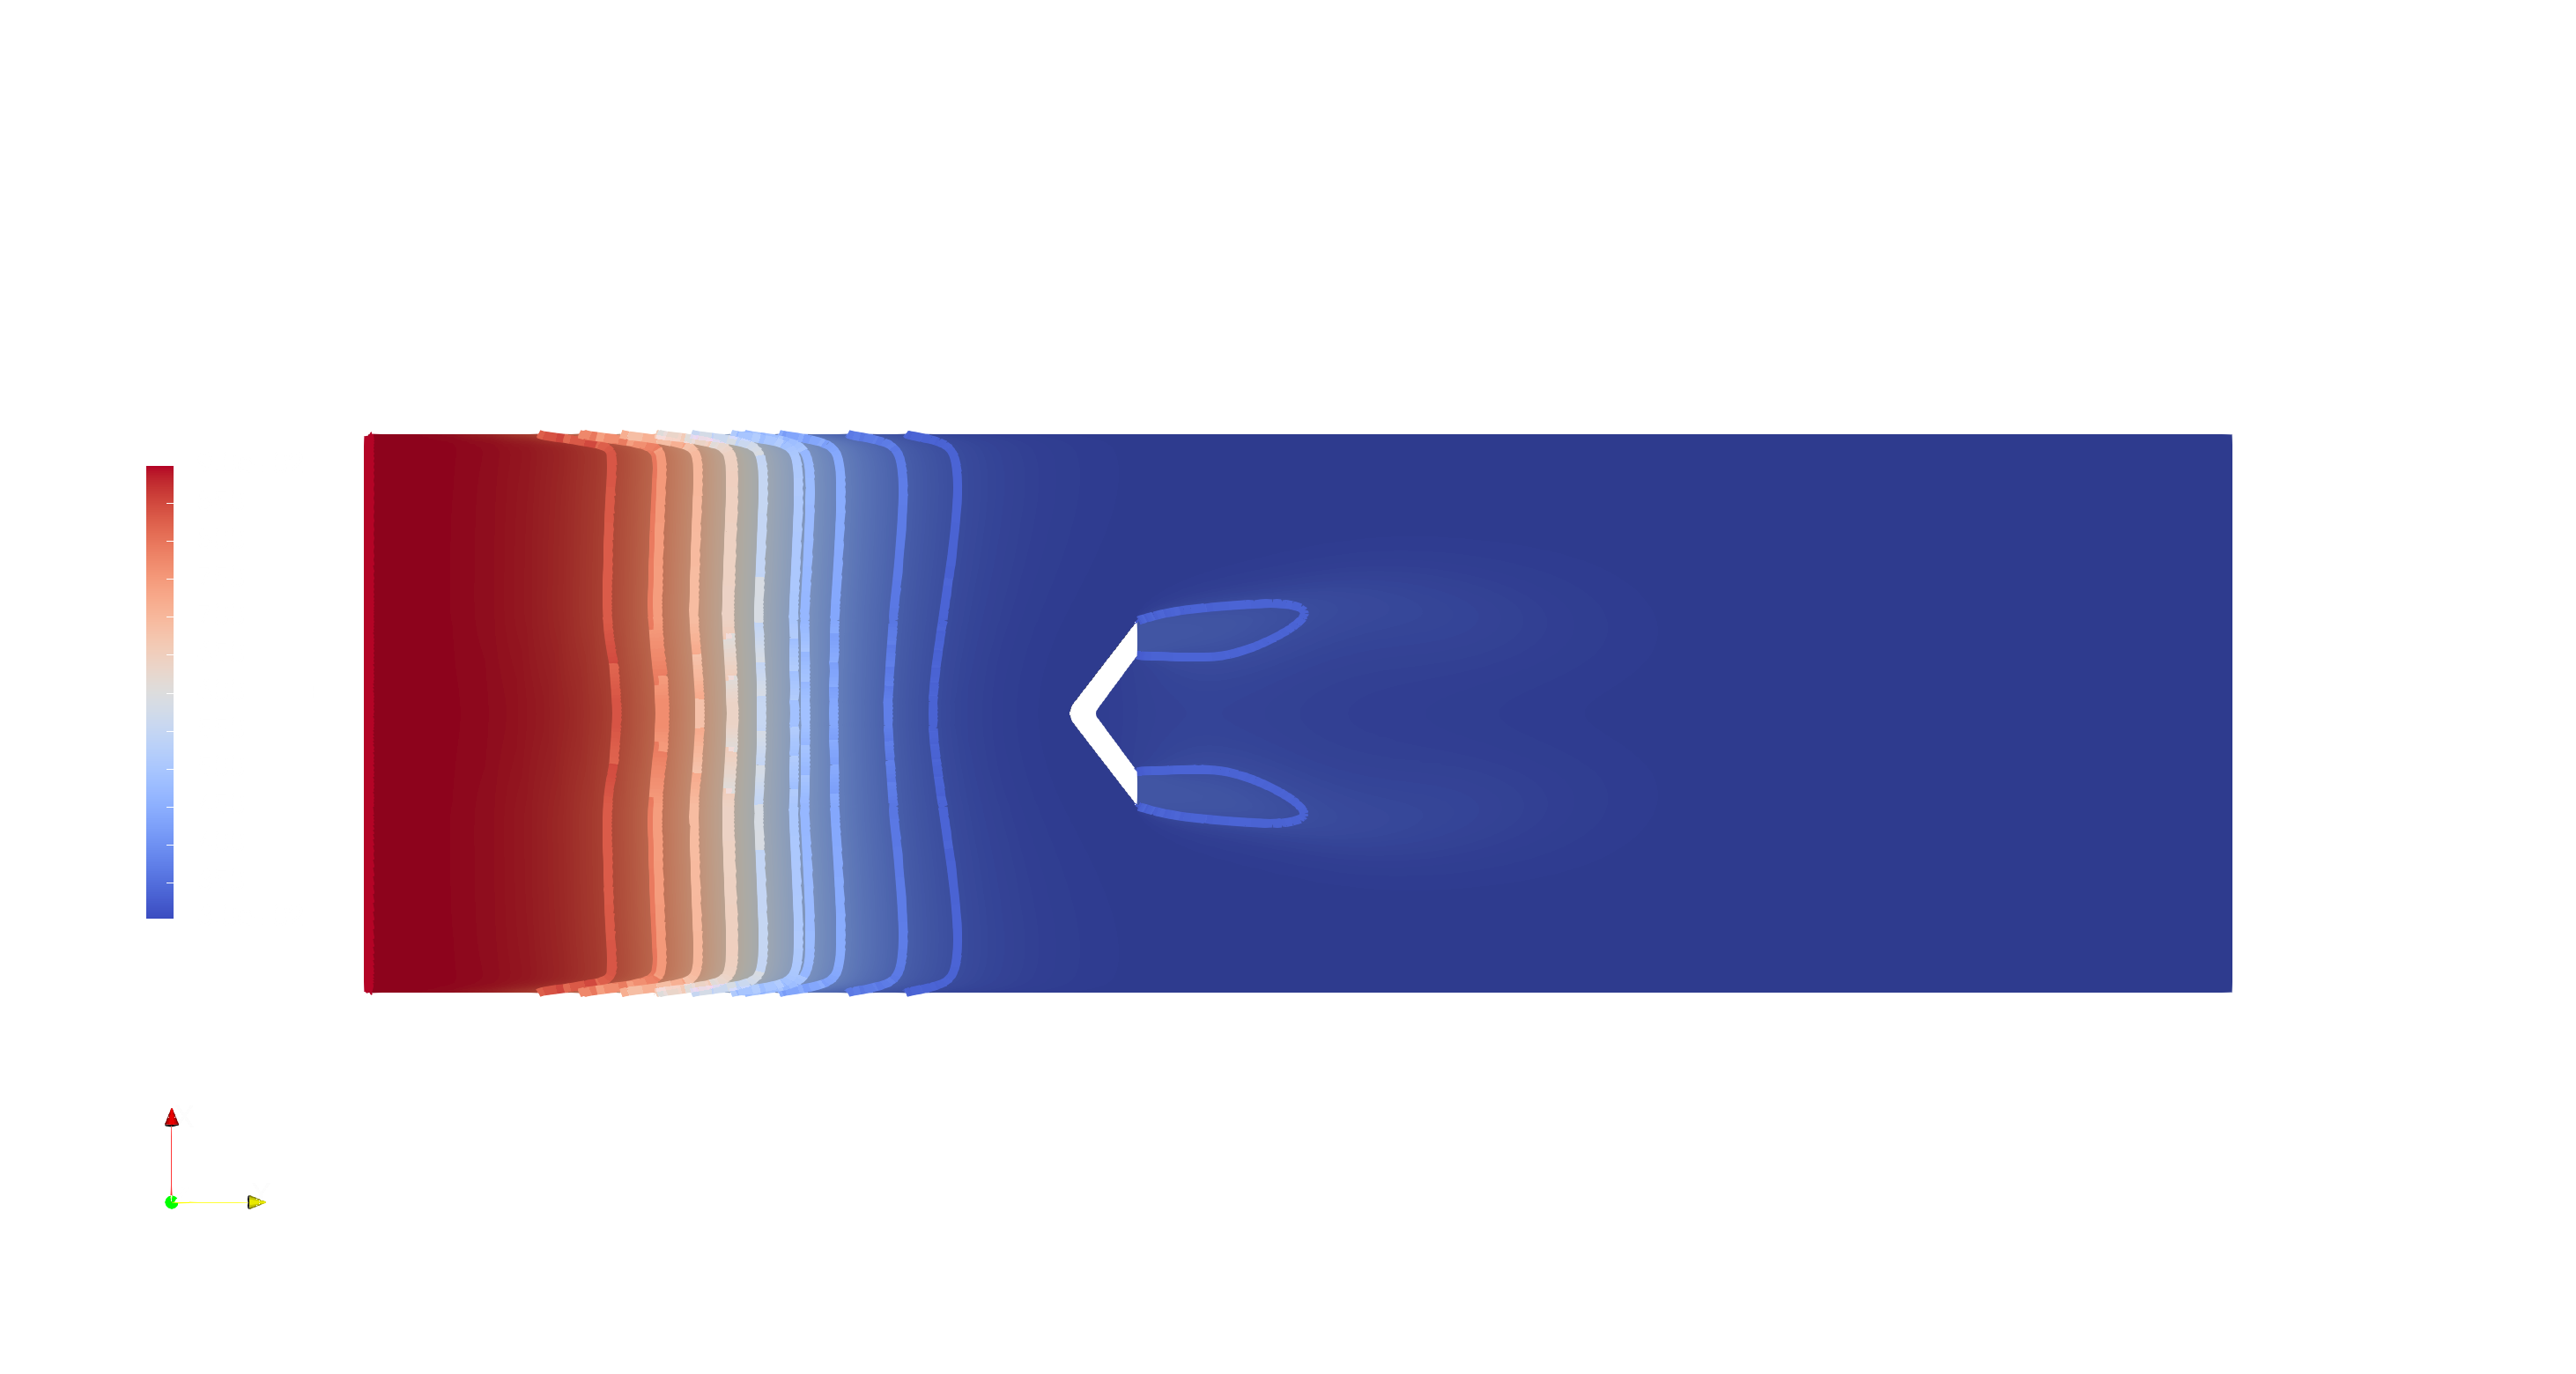
\includegraphics[height=0.25\textheight]{latexFIGS/figs/combustorT_002.png}
        \cprotect\caption{\verb|T| contour plot, $t = 0.02s$.}
    \end{figure}
    
    \begin{figure}[!h]
        \centering
        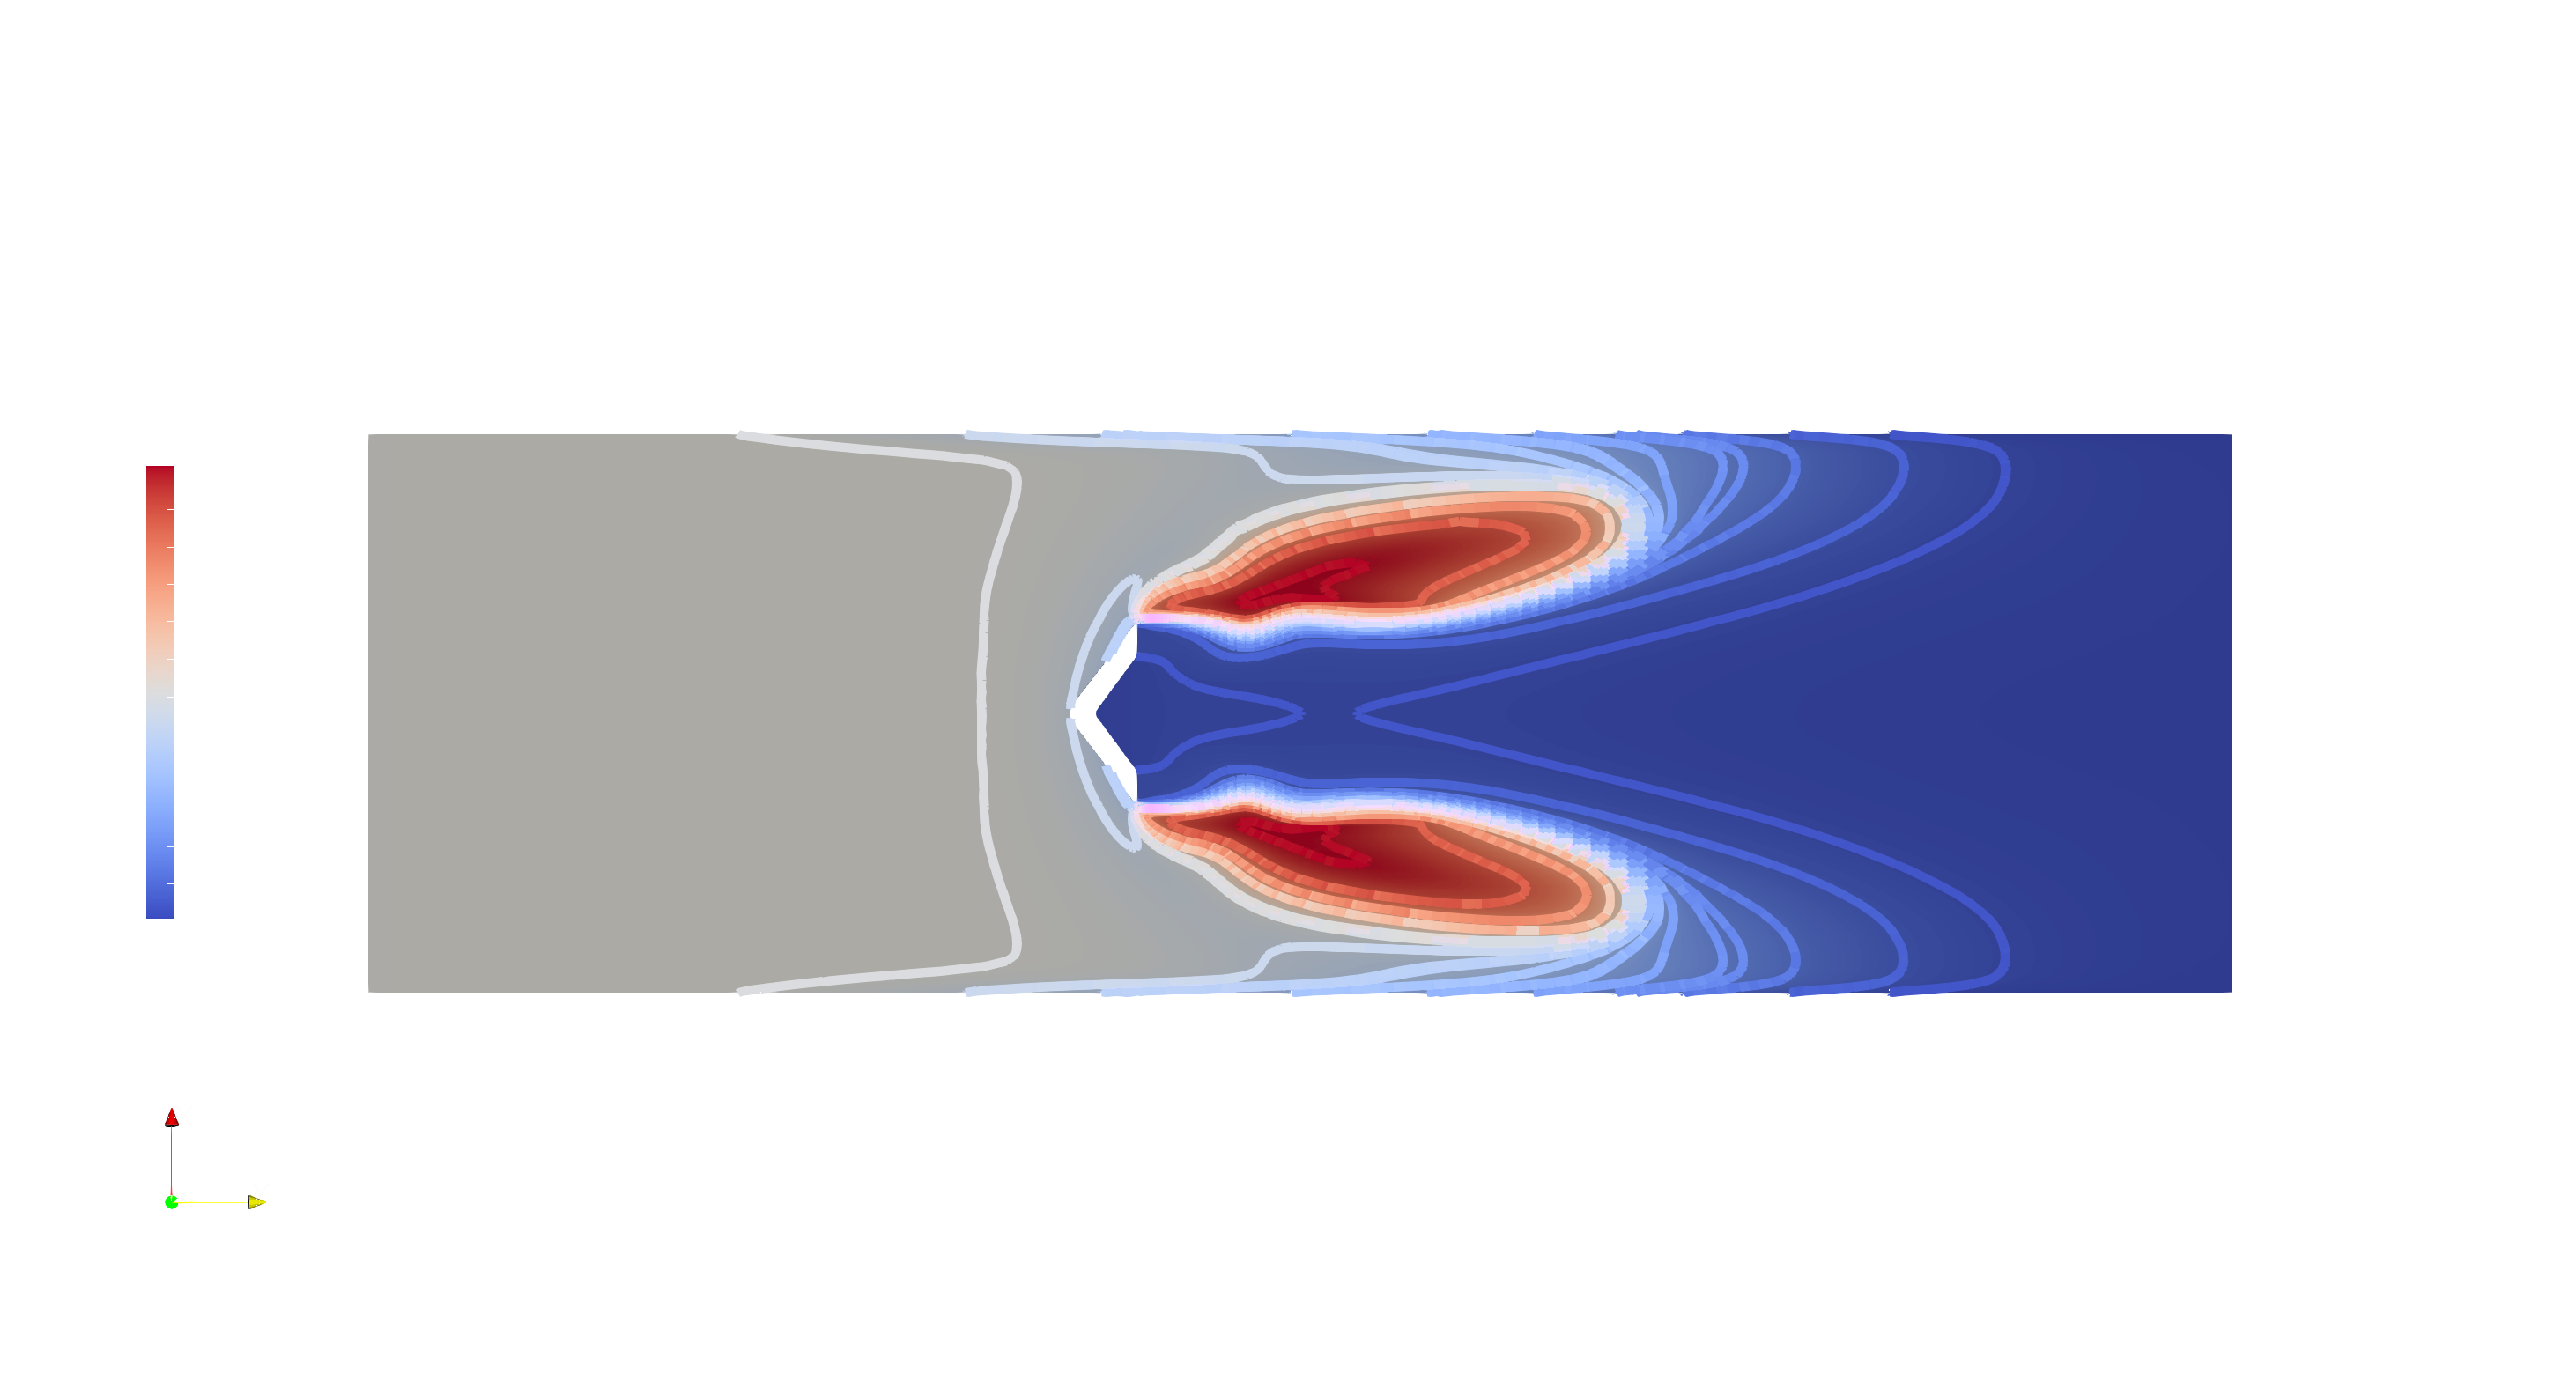
\includegraphics[height=0.25\textheight]{latexFIGS/figs/combustorT_005.png}
        \cprotect\caption{\verb|T| contour plot, $t = 0.05s$.}
    \end{figure}
    
    \begin{figure}[!hb]
        \centering
        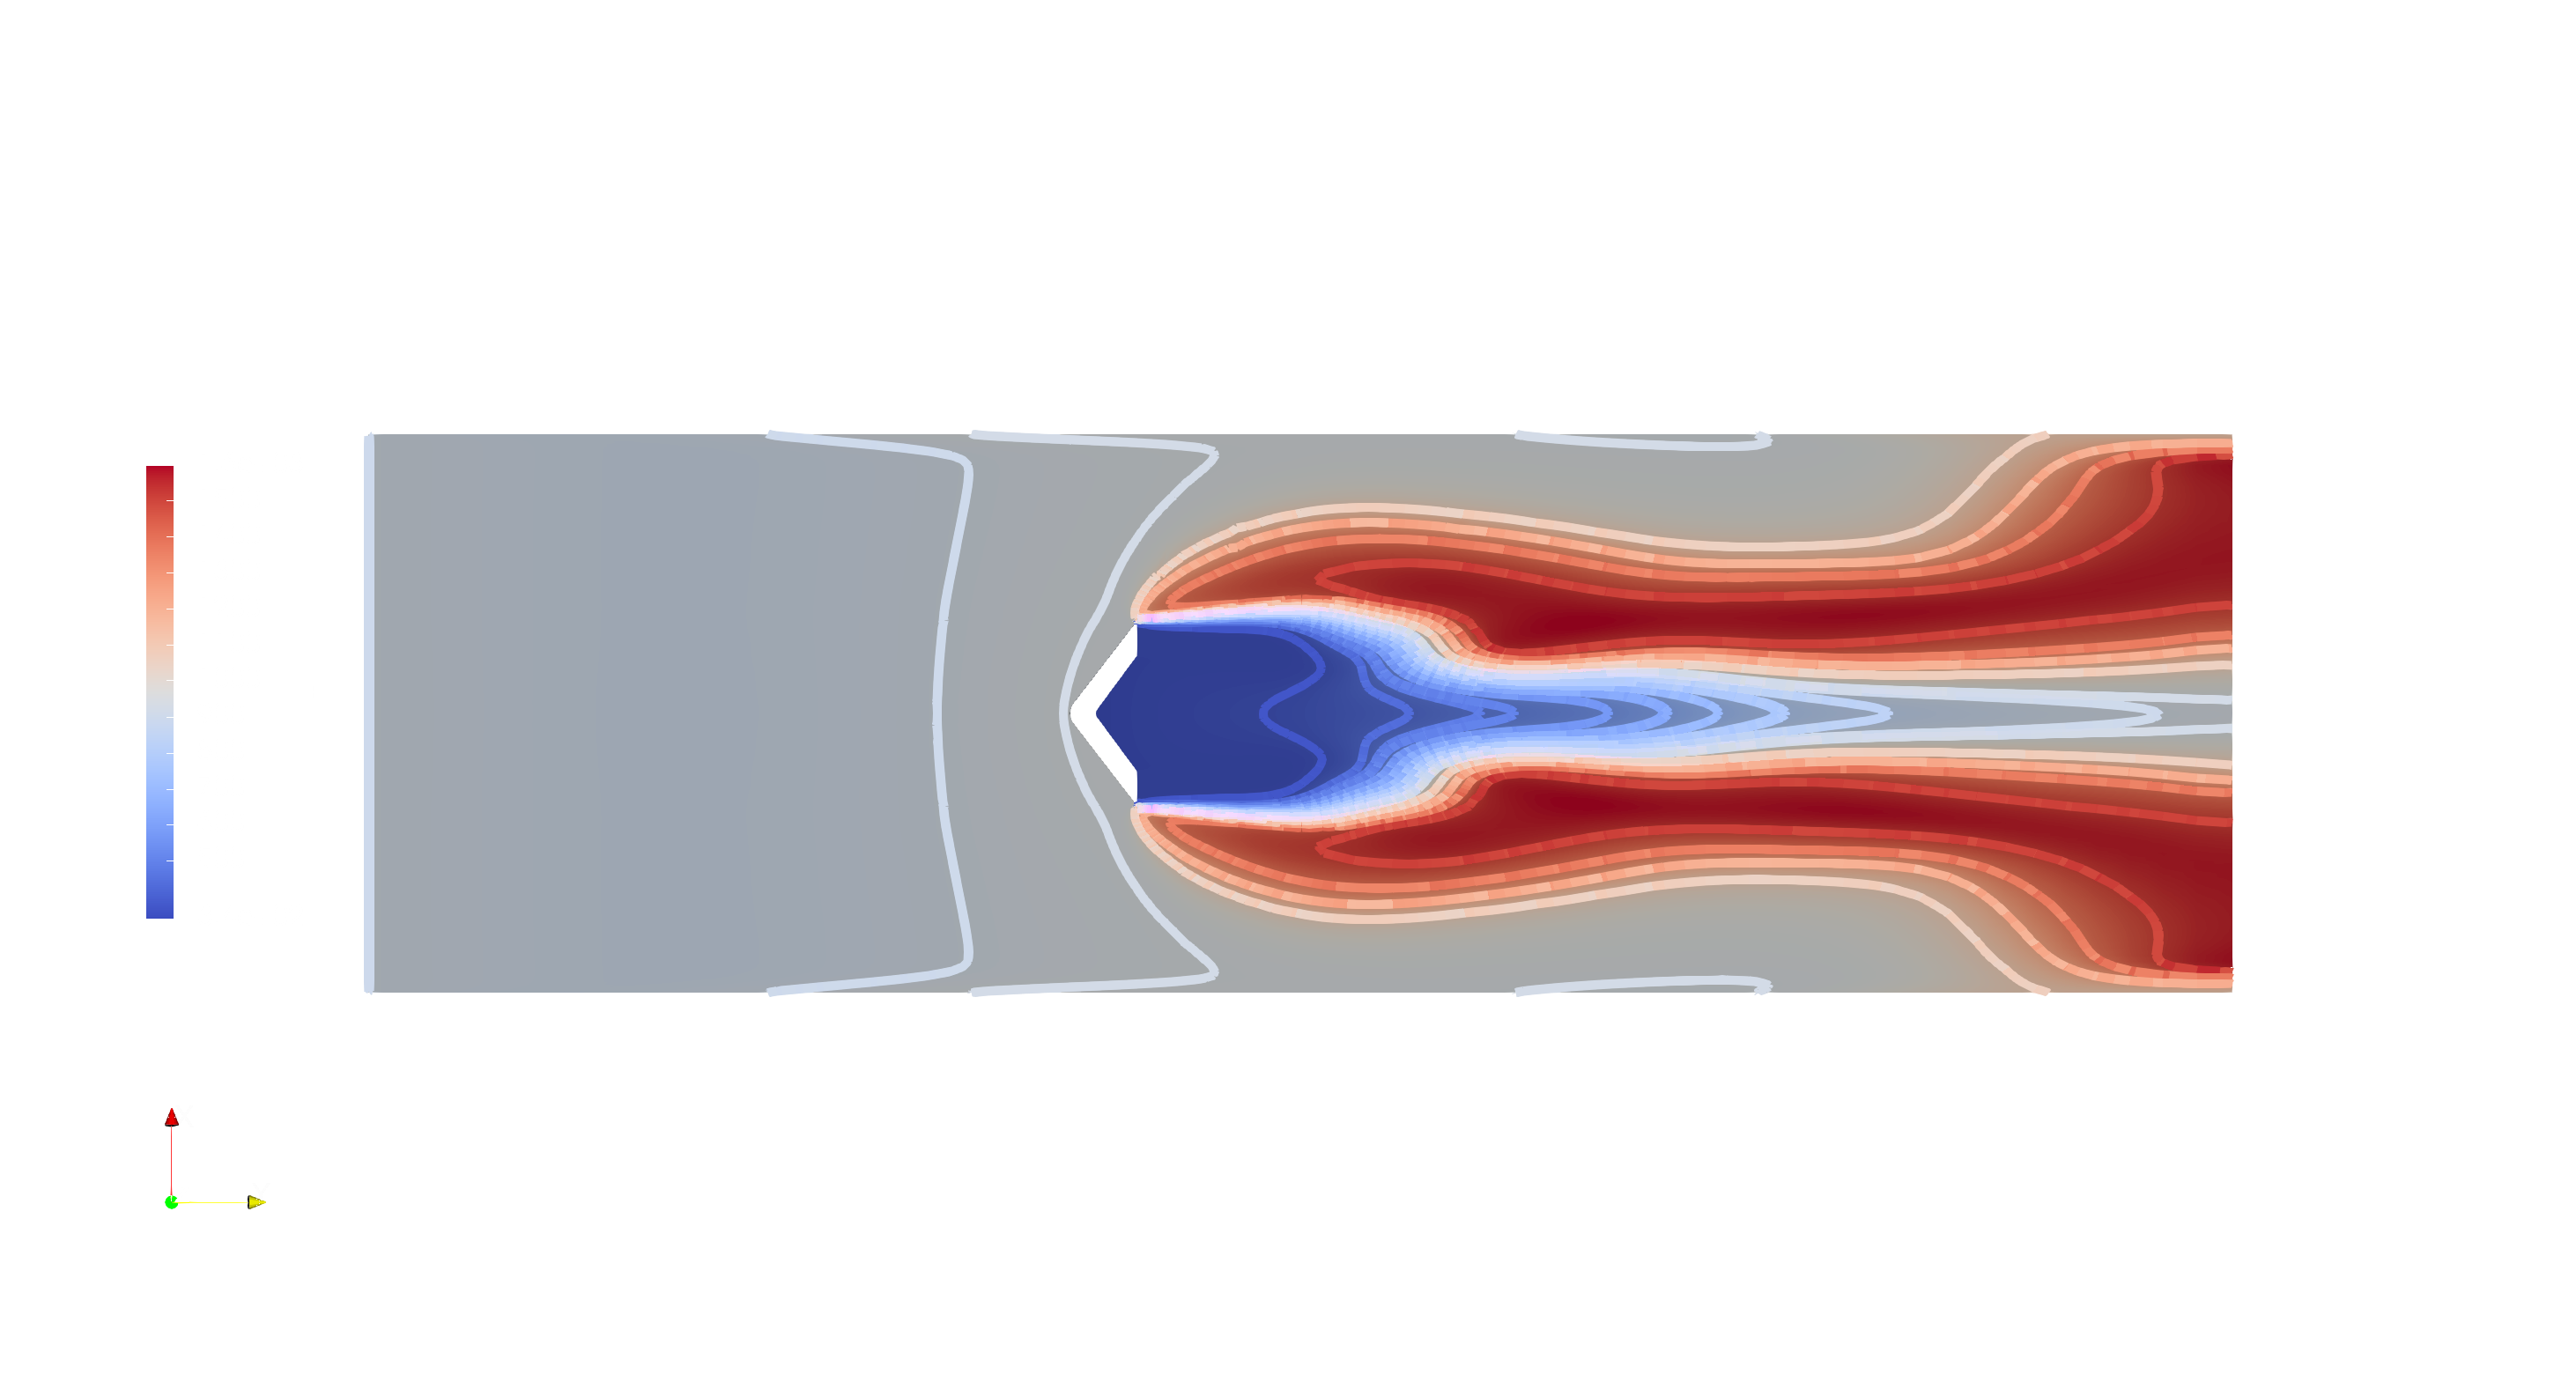
\includegraphics[height=0.25\textheight]{latexFIGS/figs/combustorT_008.png}
        \cprotect\caption{\verb|T| contour plot, $t = 0.08s$.}
    \end{figure}

    \begin{figure}[!ht]
        \centering
        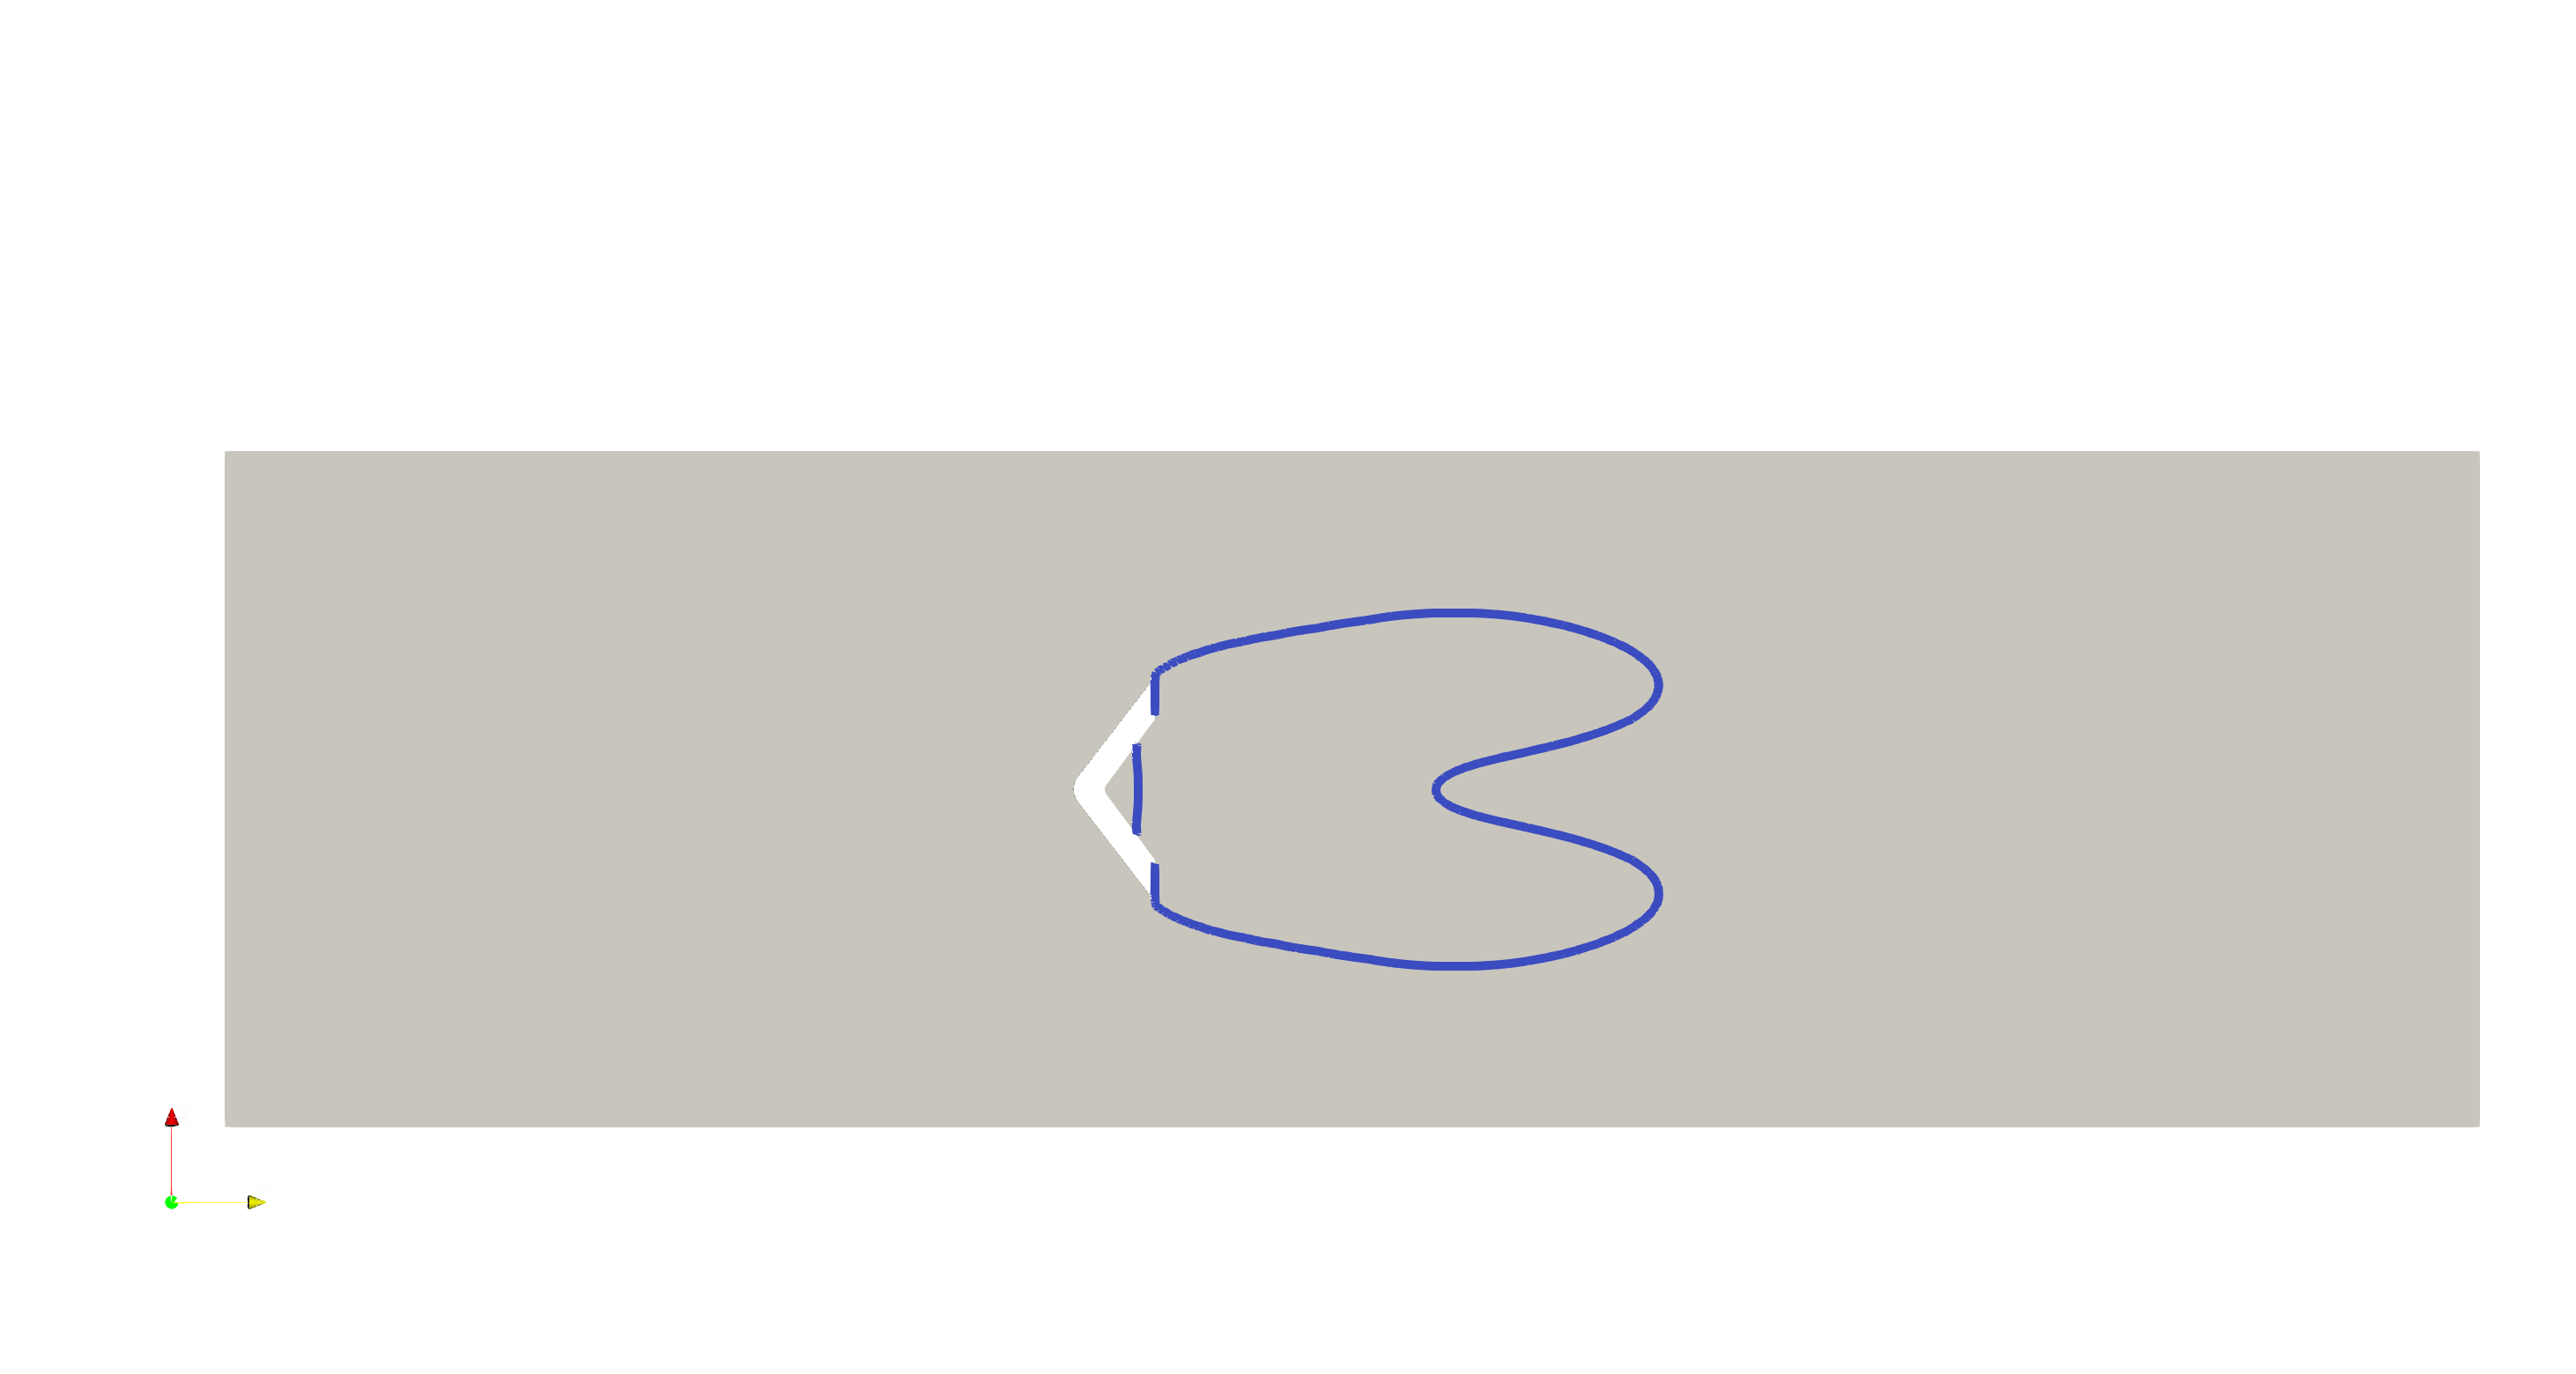
\includegraphics[height=0.25\textheight]{latexFIGS/figs/combustorSTOI1_002.png}
        \cprotect\caption{\verb|A/F| stoichiometric contour plot, $t = 0.02s$.}
    \end{figure}
    
    \begin{figure}[!h]
        \centering
        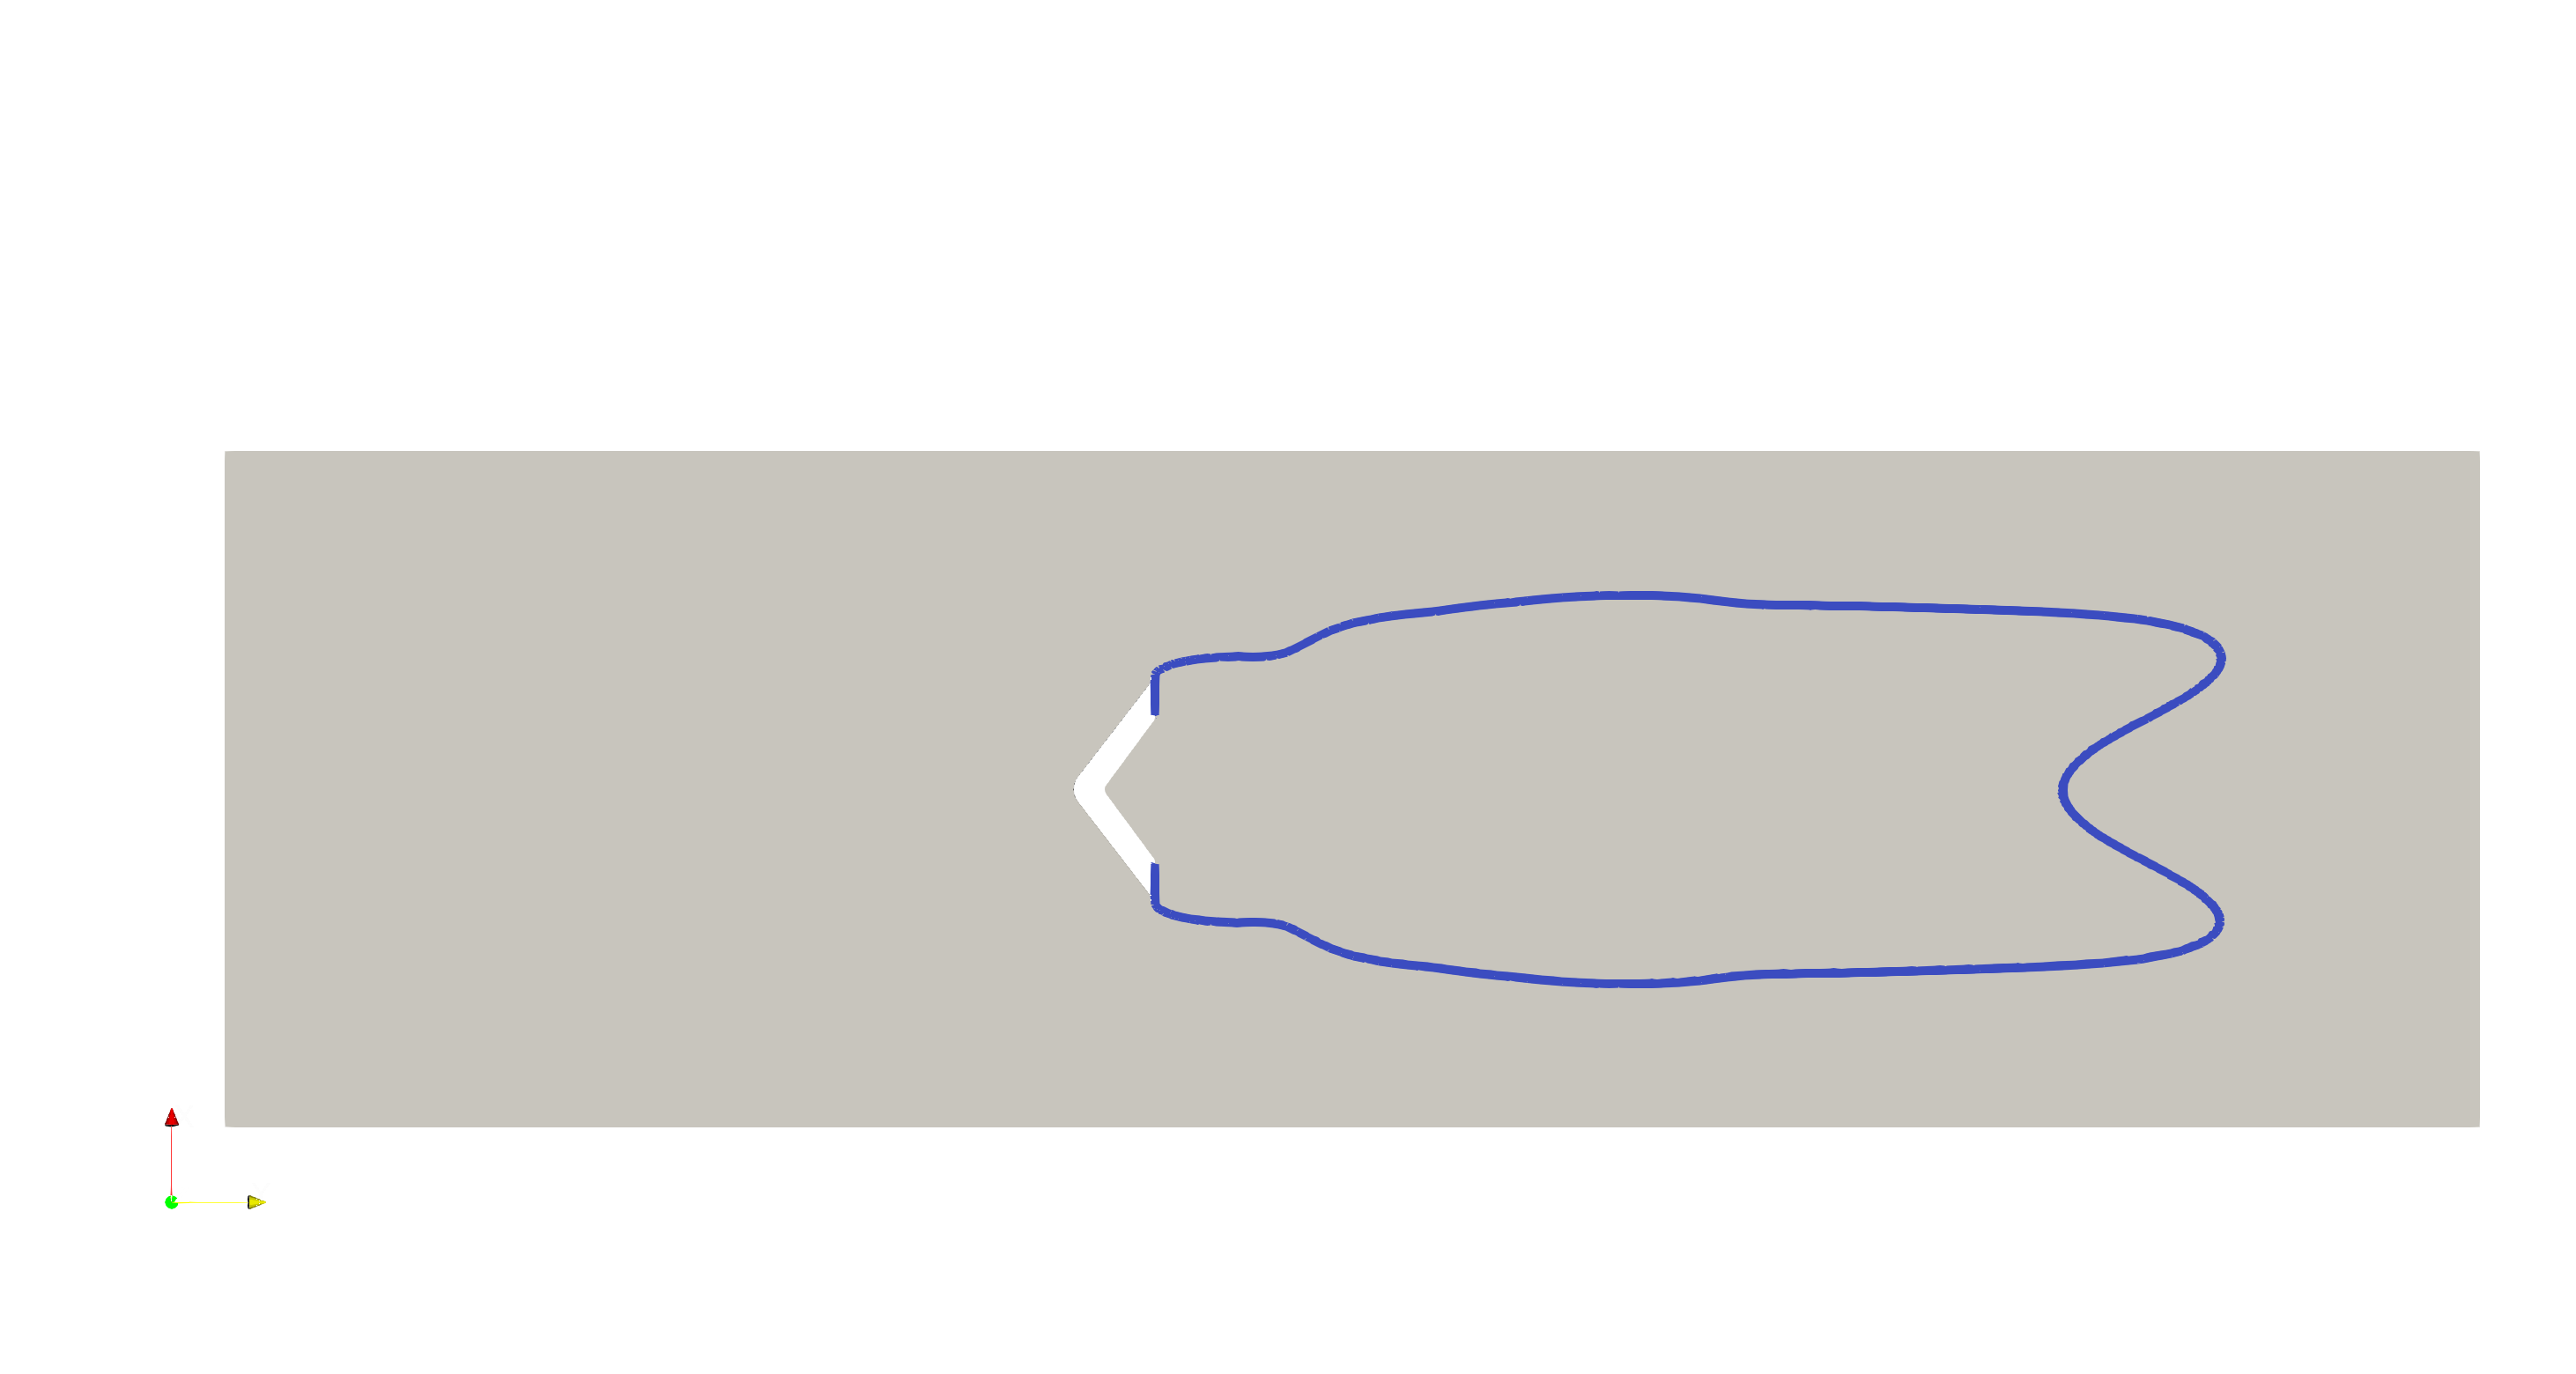
\includegraphics[height=0.25\textheight]{latexFIGS/figs/combustorSTOI1_005.png}
        \cprotect\caption{\verb|A/F| stoichiometric contour plot, $t = 0.05s$.}
    \end{figure}
    
    \begin{figure}[!hb]
        \centering
        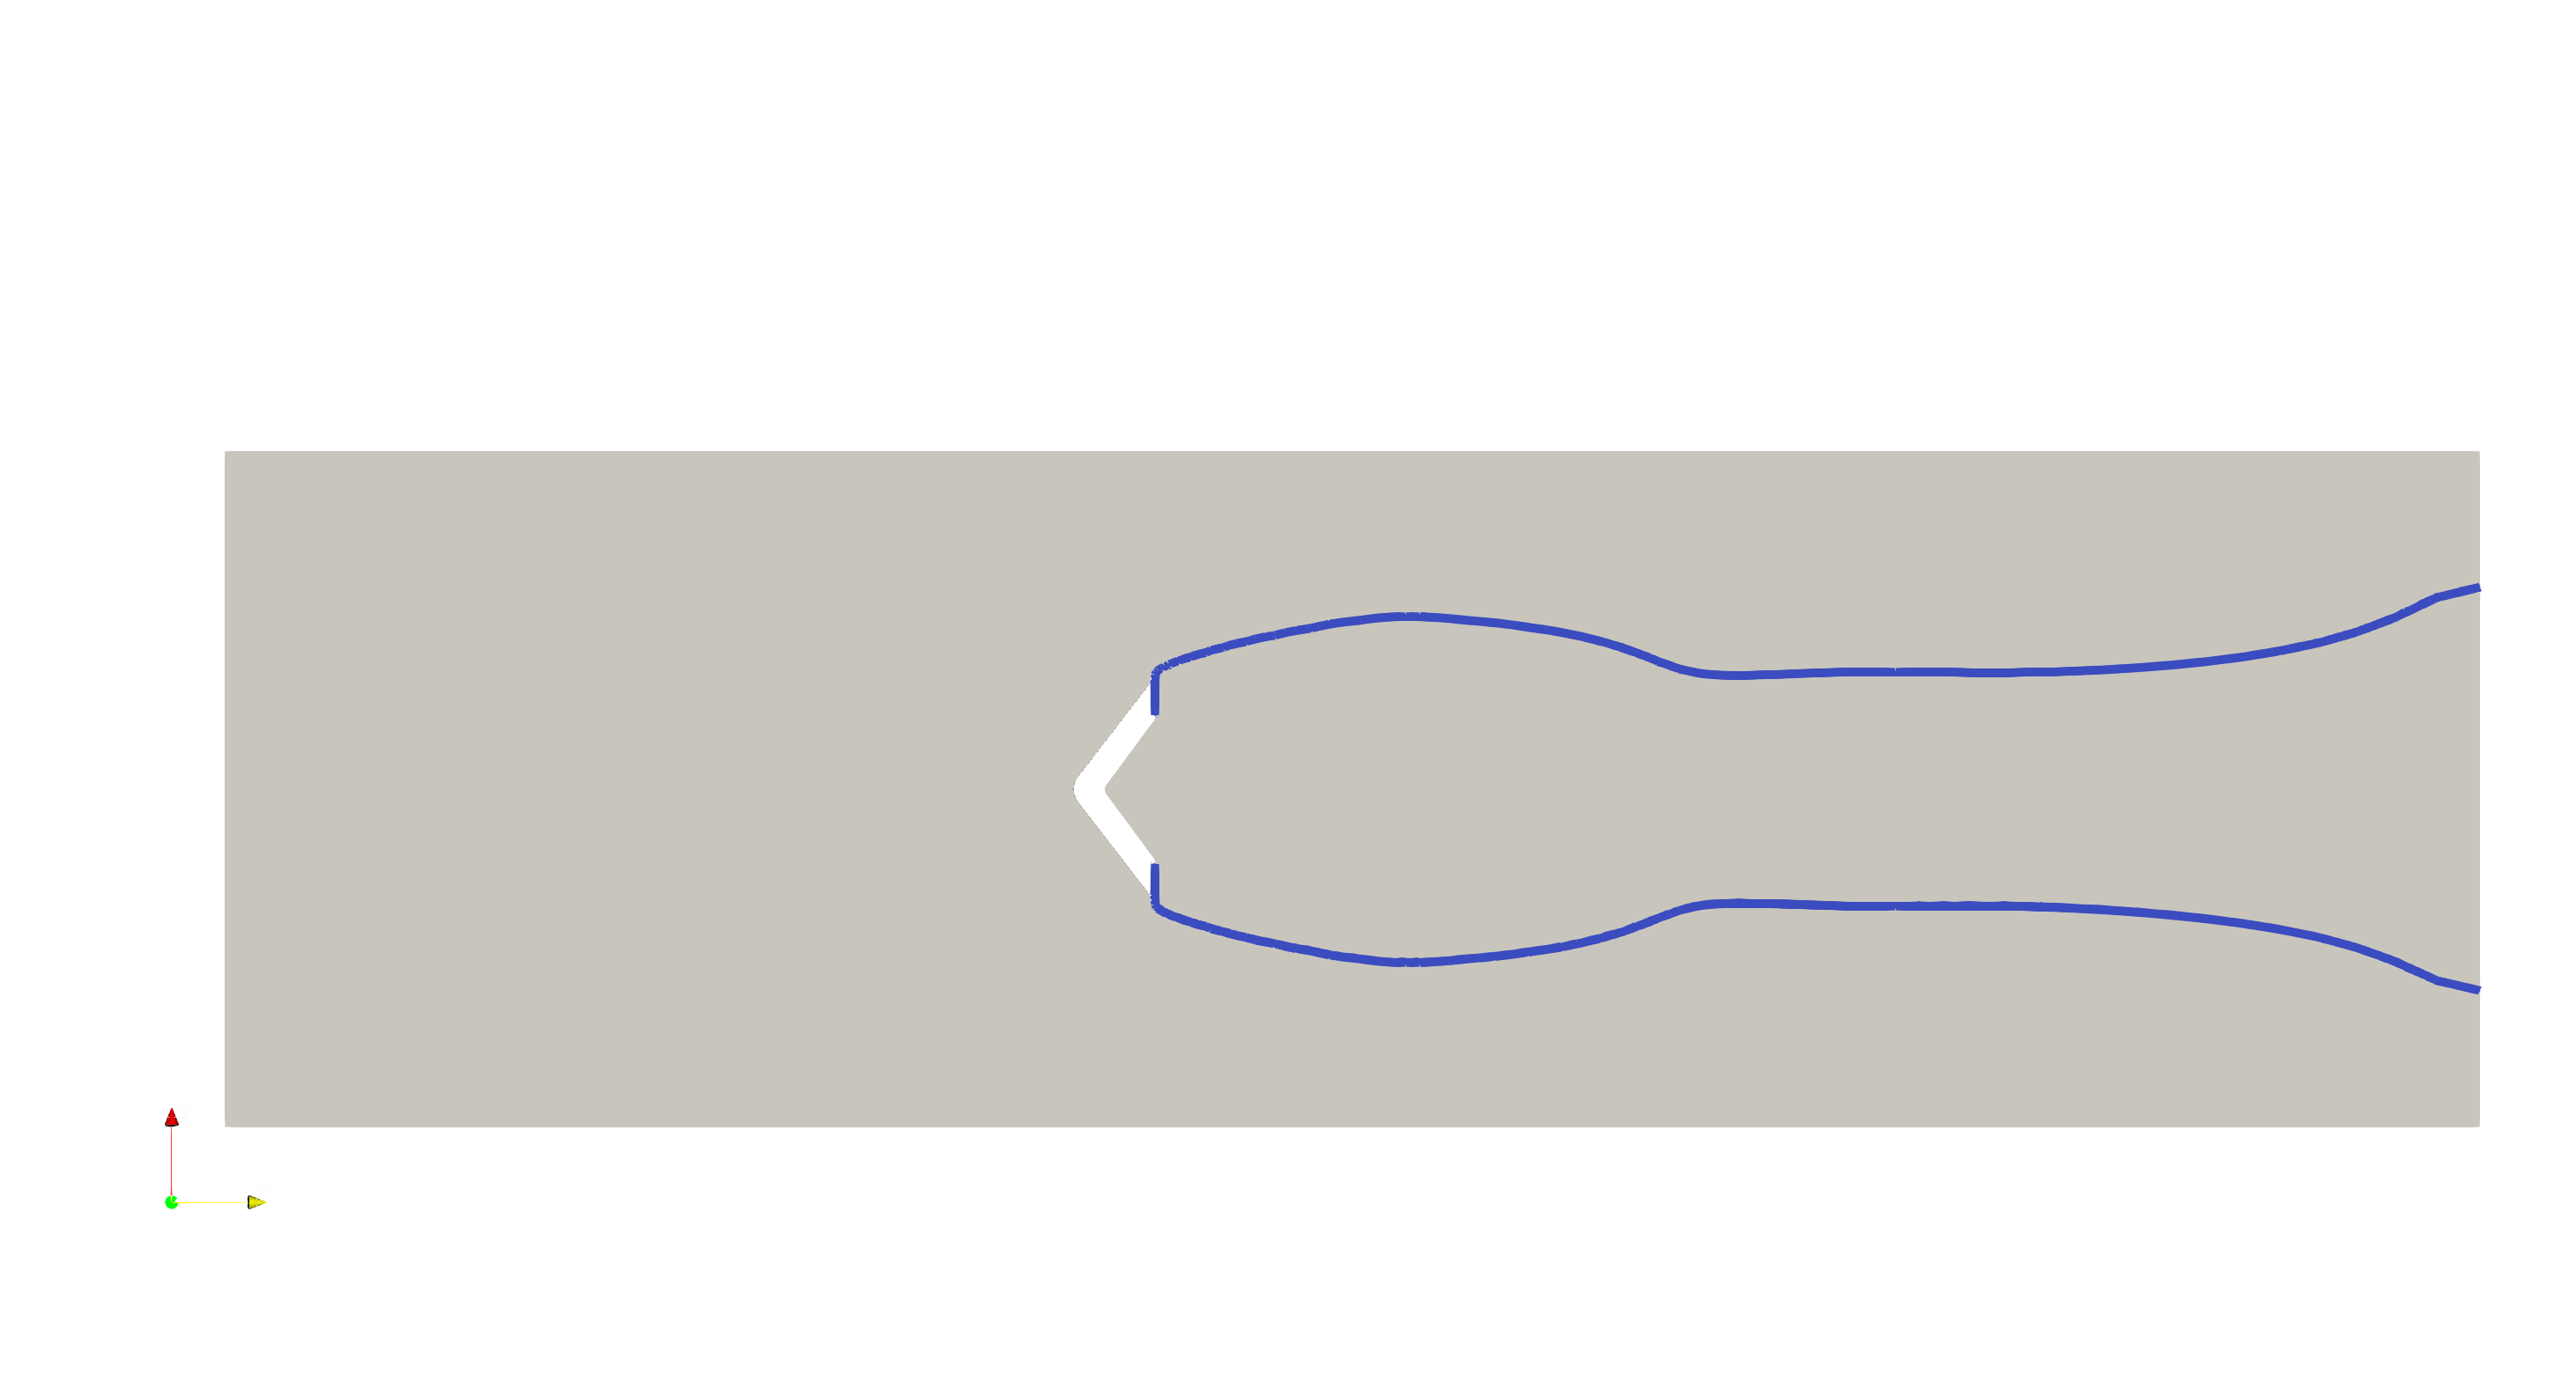
\includegraphics[height=0.25\textheight]{latexFIGS/figs/combustorSTOI1_008.png}
        \cprotect\caption{\verb|A/F| stoichimetric contour plot, $t = 0.08s$.}
    \end{figure}
    \clearpage

    \newpage
    % !TEX root = ~/OpenFOAM/antoniopucciarelli-9/run/LABS/thermochemical_CFD/main.tex

\section{Final assignment -- $\mathtt{LabAssignment}$}
    
    \renewcommand{\thepage}{\arabic{page}}
    \setcounter{page}{\thelastPage}
    
    This last case treats the analysis of the 3D combustor. 

    The main difference among this case and the 2D cases is the computational cost related to the additional coordinate of study. Convergence parameters are set up in order to reduce the computational time and ensuring good results. 

    \subsection{Problem setup}
    \subsubsection{Boundary conditions}
    The main difference between the 2D case is the fact that there is no more the \verb|frontAndBack| patch. The \verb|frontAndBack| patch is changed with \verb|outerWalls| patch. 
    Because it is no more a 2D problem, the \verb|outerWalls| does not use the \verb|empty| type for the boundary conditions on every variables' dictionary. 

    \cprotect\subsubsection{\verb|fvModels|}
    This dictionary activates \textit{only} the lagrangian spray modeling. The liquid film modeling is not activated due to the computational resources available.
    \begin{lstlisting}[caption = $\mathtt{combustorReaction/constant/fvModels}$ activates only lagrangian spray model and the bouyancy forces., label = list:fvModels]
            buoyancyForce
            {
                type    buoyancyForce;
            }

            clouds
            {
                type    clouds;
                libs    ("liblagrangianParcel.so");
            }

            //surfaceFilm
            //{
            //    type    surfaceFilm;
            //    libs    ("libsurfaceFilmModels.so");
            //}
    \end{lstlisting}
    
    \cprotect\subsubsection{\verb|chemistryProperties|}
    As in \verb|Lab07| chemistry solver is described in \verb|chemistryProperties| and the solver used is the \verb|seulex| solver. The reaction properties data are taken from \verb|reactions| dictionary where the \verb|C7H16|-air reaction is modeled as \verb|irreversibleArrhenius|. 

    \cprotect\subsubsection{\verb|combustionProperties|} 
    As in \ref{sec:PaSR}, due to characteristic time of the reaction with respect to the \textit{main} flow characteristic time, \verb|PaSR| combustion model is used for the combustion modeling. The \verb|PaSR| model considers turbulence for the combustion modeling. 

    \cprotect\subsubsection{\verb|thermophysicalProperties|}
    This dictionary takes into account the presence of liquid \verb|C7H16| into the system - because the presence of spray -, this will bring as setting \verb|C7H16| in the \verb|liquid| subdictionary. As in \ref{sec:speciesThermo}, species thermodynamics properties are taken from \verb|speciesThermo|\cprotect\footnote{For \verb|Lab07|, \verb|thermophysicalProperties| takes the thermodynamic properties of each species from the \verb|thermo.mixture| dictionary, that is a copy of \verb|speciesThermo|. In the \verb|Lab-Assignemnt|, thermodynamic properties are recovered directly from \verb|speciesThermo|.}.
    
    \cprotect\subsubsection{\verb|fvSolution|}
    In order to reduce computational time for each time step, it has been used this setting:
    \begin{lstlisting}[caption = $\mathtt{combustorReaction/system/fvSolution}$ convergence setting., label = list:convergence]
        outerCorrectorResidualControl
        {
            p
            {
                tolerance   5e-03;
                relTol      0.0;
            }

            U
            {
                tolerance   5e-04;
                relTol      0.0;
            }

            h
            {
                tolerance   5e-04;
                relTol      0.0;
            }
        }

        residualControl
        {
            p   5e-03;
            U   5e-04;
            h   5e-04;
        }
    \end{lstlisting}
    The maximum number of number of outer correctors is $150$ and the turbulence models are solved for each outer corrector step, \verb|turbOnFinalIterOnly false;|, based on $\kappa - \varepsilon$ model.

    \subsection{Post-processing}
    \cprotect\subsubsection{\verb|surfaceFieldValue|}
    In order to compute field average on \verb|inlet| and \verb|outlet| patches, the \verb|surfaceFieldValue| function is used. Pressure and temperature are the averaged patch fields. The \verb|writeInterval 1e-02;| is set in order to reduce the space occupied on the memory\footnote{The simulation occupies at the end of the simulation almost $3GB$.}. 

    \subsection{Results}
        \cprotect\subsubsection{\verb|combustorRhoPimple|}
        This case is used for the initialization of the flow in the combustor case. It has been used a \verb|maxCo 5;| for the simulation in order to get good initial conditions for the combustion in the shortest time possible. Of course, \verb|maxCo 5;| can filter a bit too much the field but, with the computational power available, it has been preferred to use a bit finer mesh\footnote{Around $1 \cdot 10^6$ cells.} to a low Courant number\cprotect\footnote{Having a low Courant number with coarse mesh is useless because a coarse mesh can be seen as a spacial filter of the results - as well as high Courant number can be seen as a temporal filter on the solution -. Although \verb|RANS| are based on time filtering, an high Courant number (that is just related to numerics) can be seen as a \textbf{numerical model filter}.}.
        
        \cprotect\subsubsection{\verb|combustorReaction|}
        The time spent for the solution of this case is around $3$ days. Convergence is reached for every time step and the simulation results are shown below. Although the lack of the surface film modeling, spray interaction with the \textit{main} flow and the \verb|C7H16| combustion is present in the final solution. Combustion happens mainly at the end of the splitter after the mixing and evaporation of the \verb|C7H16| spray with the air.    

    \newpage

    % PAGE MANAGEMENT
    % saving page number
    \setcounter{lastPage}{\thepage}
    % changing page numbering for the results figures
    \setcounter{page}{1}
    \renewcommand{\thepage}{3DR-\roman{page}}

    \begin{figure}[!ht]
        \centering
        \import{latexFIGS/labAssignment/}{residuals.pgf.bak}
        \cprotect\caption{3D case \verb|rhoPimpleFoam| and \verb|reactingFoam|: residuals.}
    \end{figure}

    \begin{figure}[!ht]
        \centering
        \import{latexFIGS/labAssignment/}{figTot.pgf.bak}
        \cprotect\caption{\verb|reactingFoam| case: liquid penetration, parcels diameter and $(p, T)$ average at inlet.} 
    \end{figure}

    \begin{figure}[!ht]
        \centering
        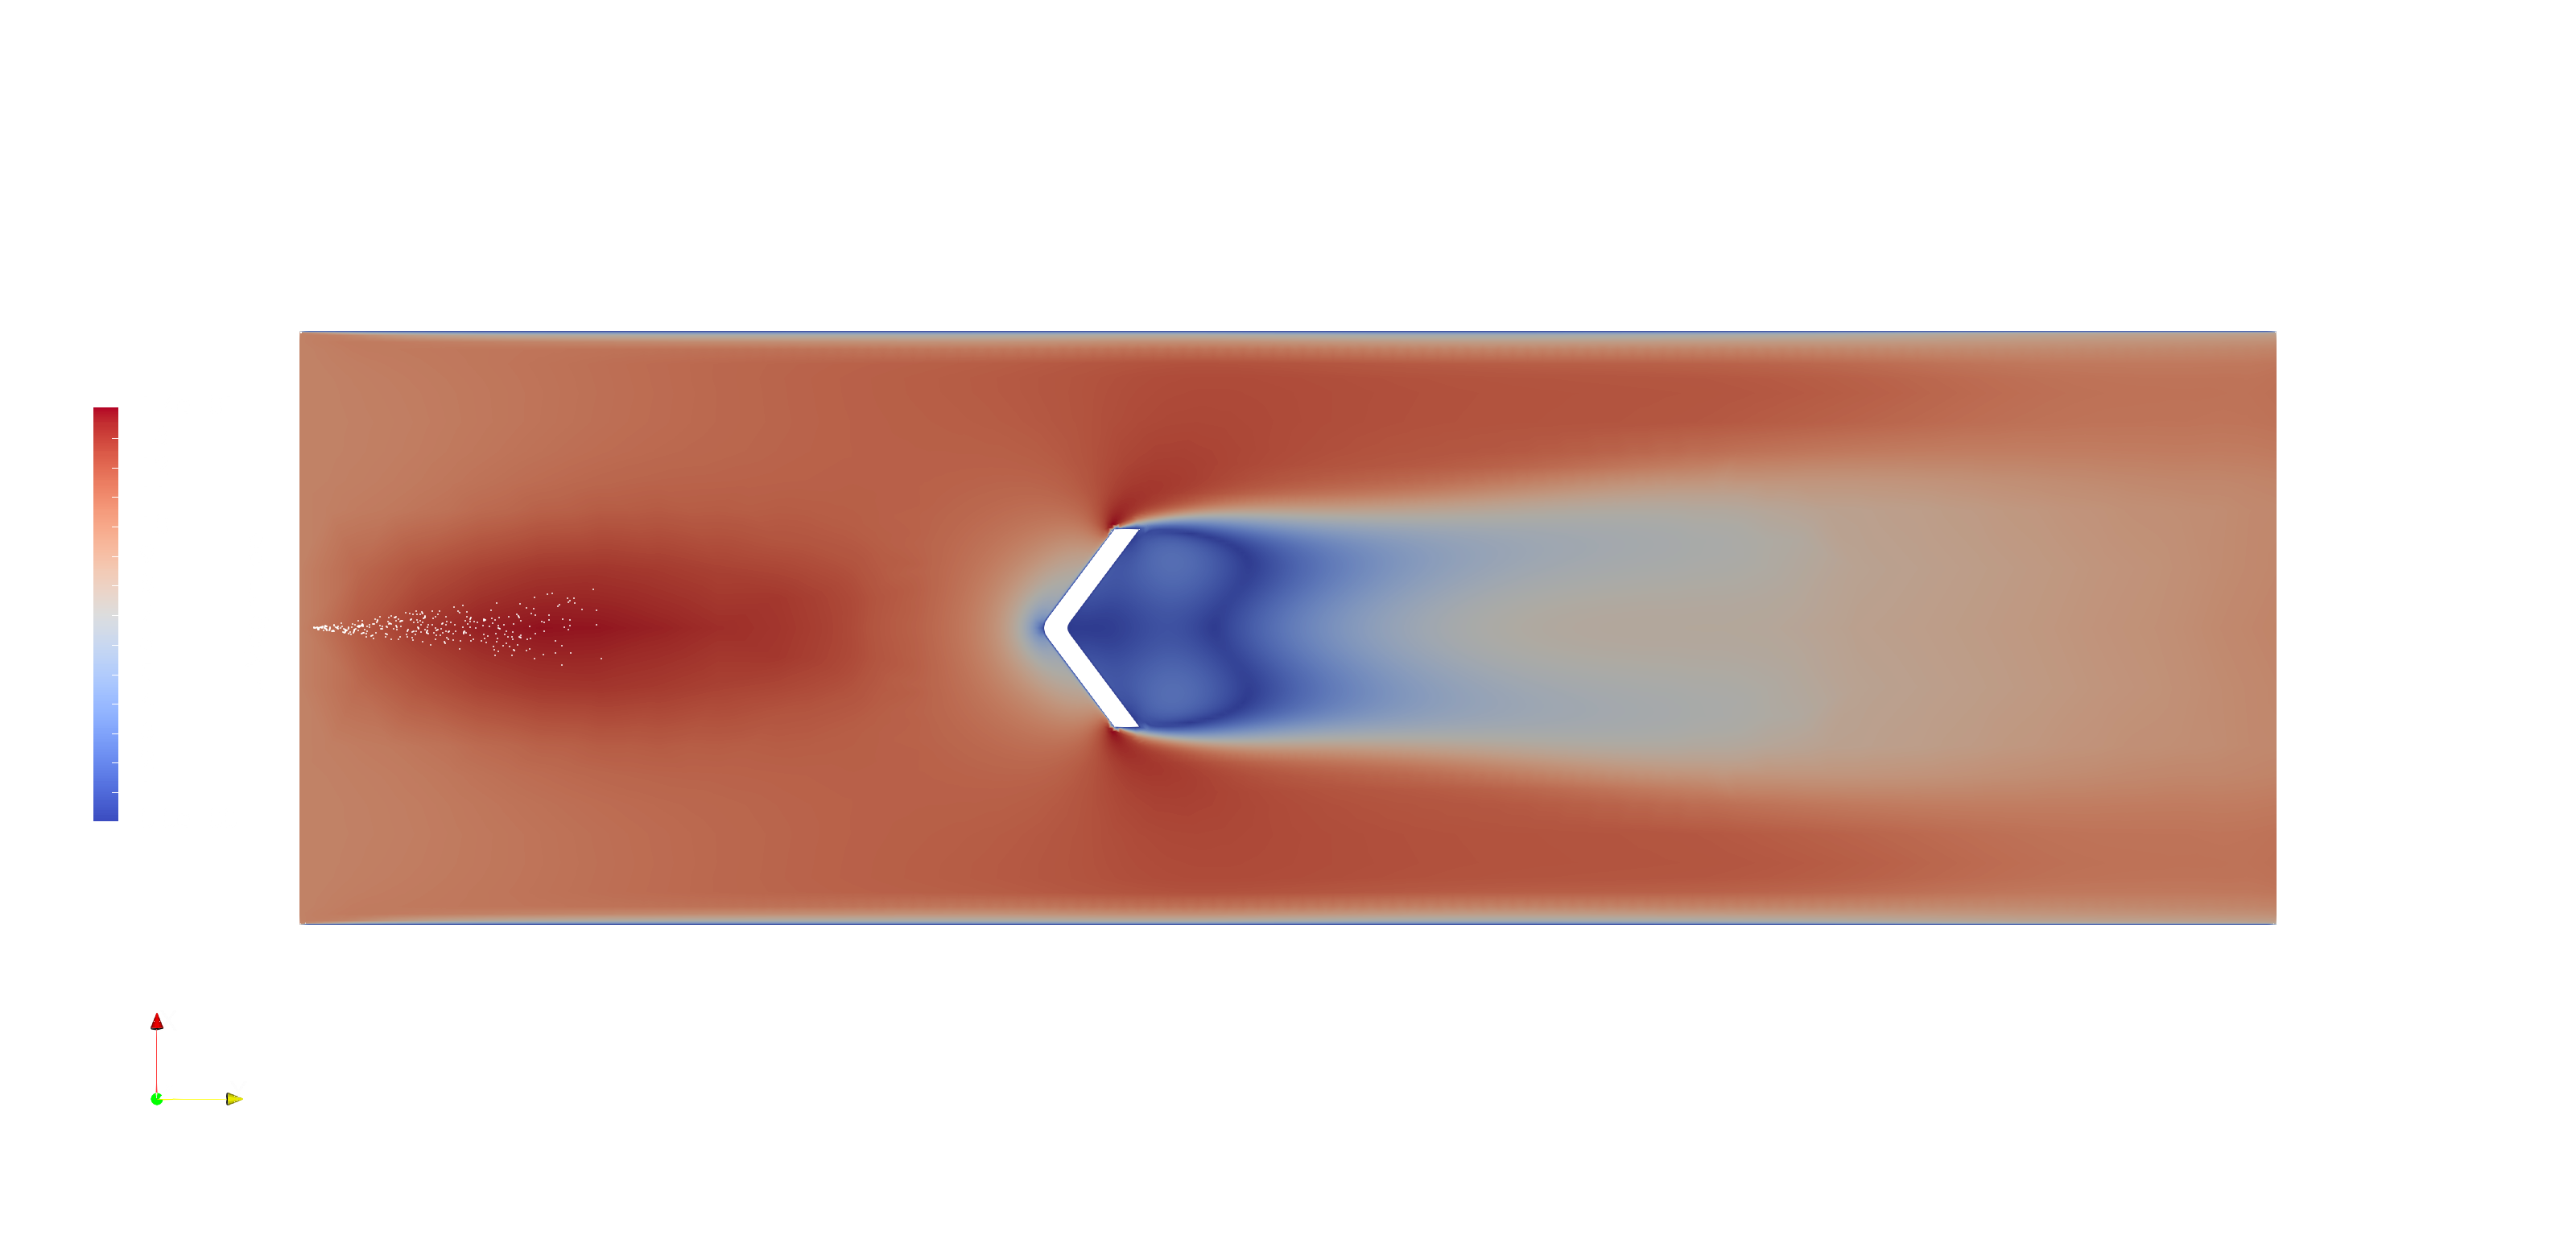
\includegraphics[width=0.8\textwidth]{latexFIGS/labAssignment/figU_02.png}
        \caption{3D reaction case: $|U|$ profile, $t = 0.02s$.}
    \end{figure}

    \begin{figure}[!ht]
        \centering
        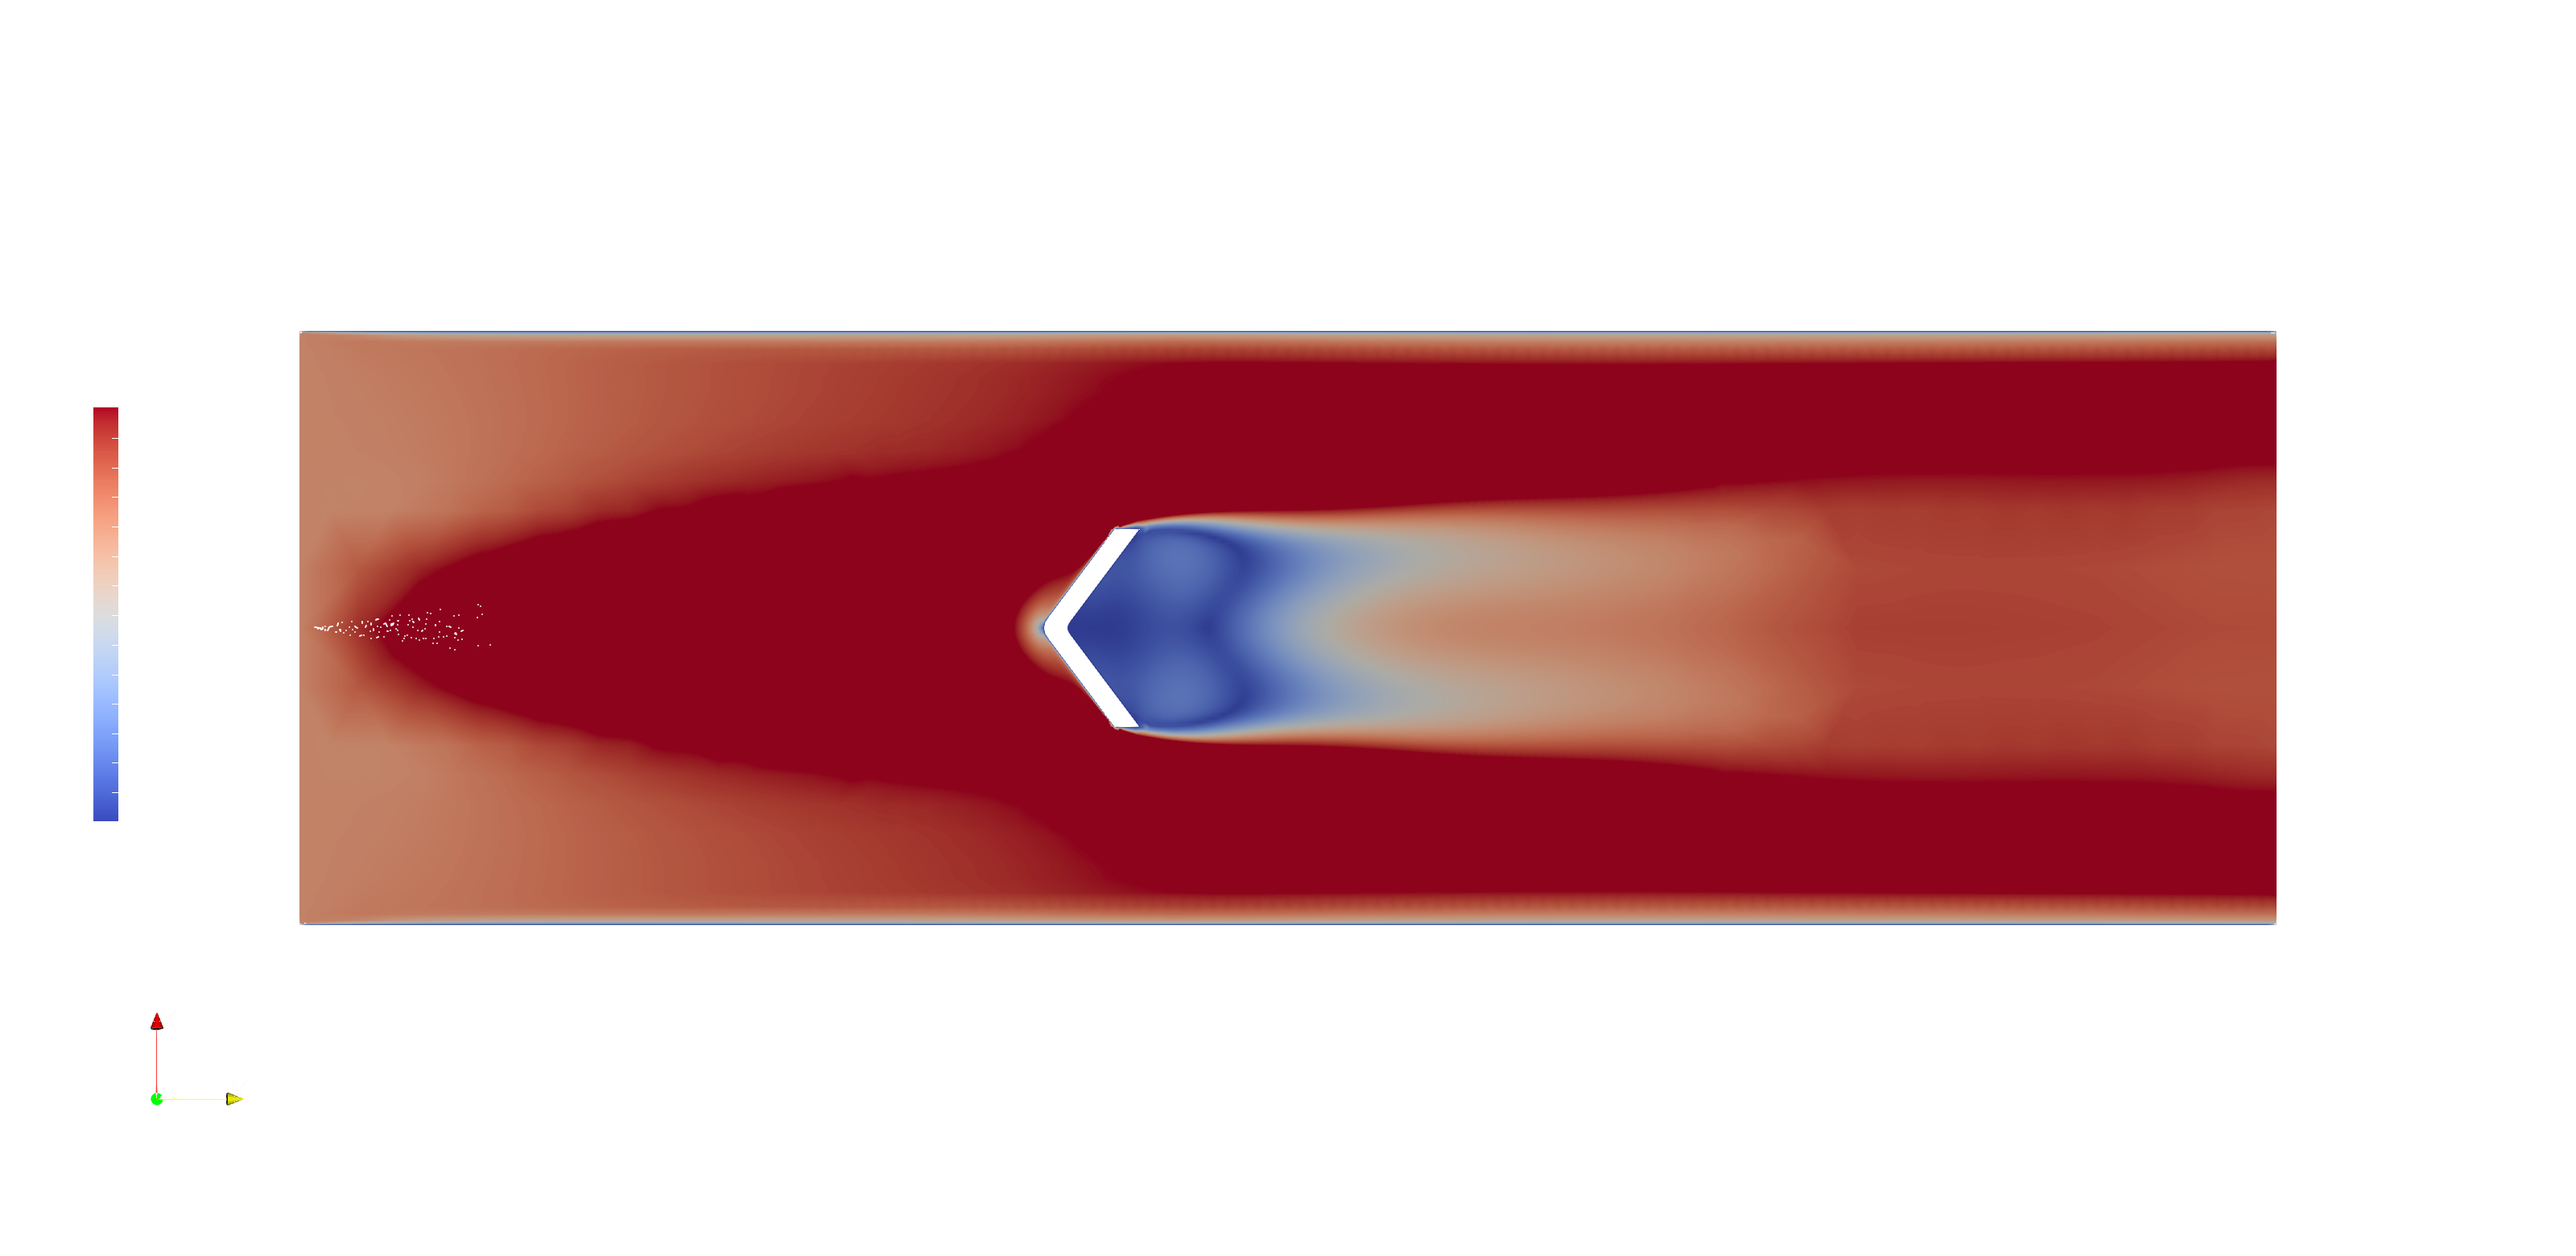
\includegraphics[width=0.8\textwidth]{latexFIGS/labAssignment/figU_05.png}
        \caption{3D reaction case: $|U|$ profile, $t = 0.05s$.}
    \end{figure}
    
    \begin{figure}[!ht]
        \centering
        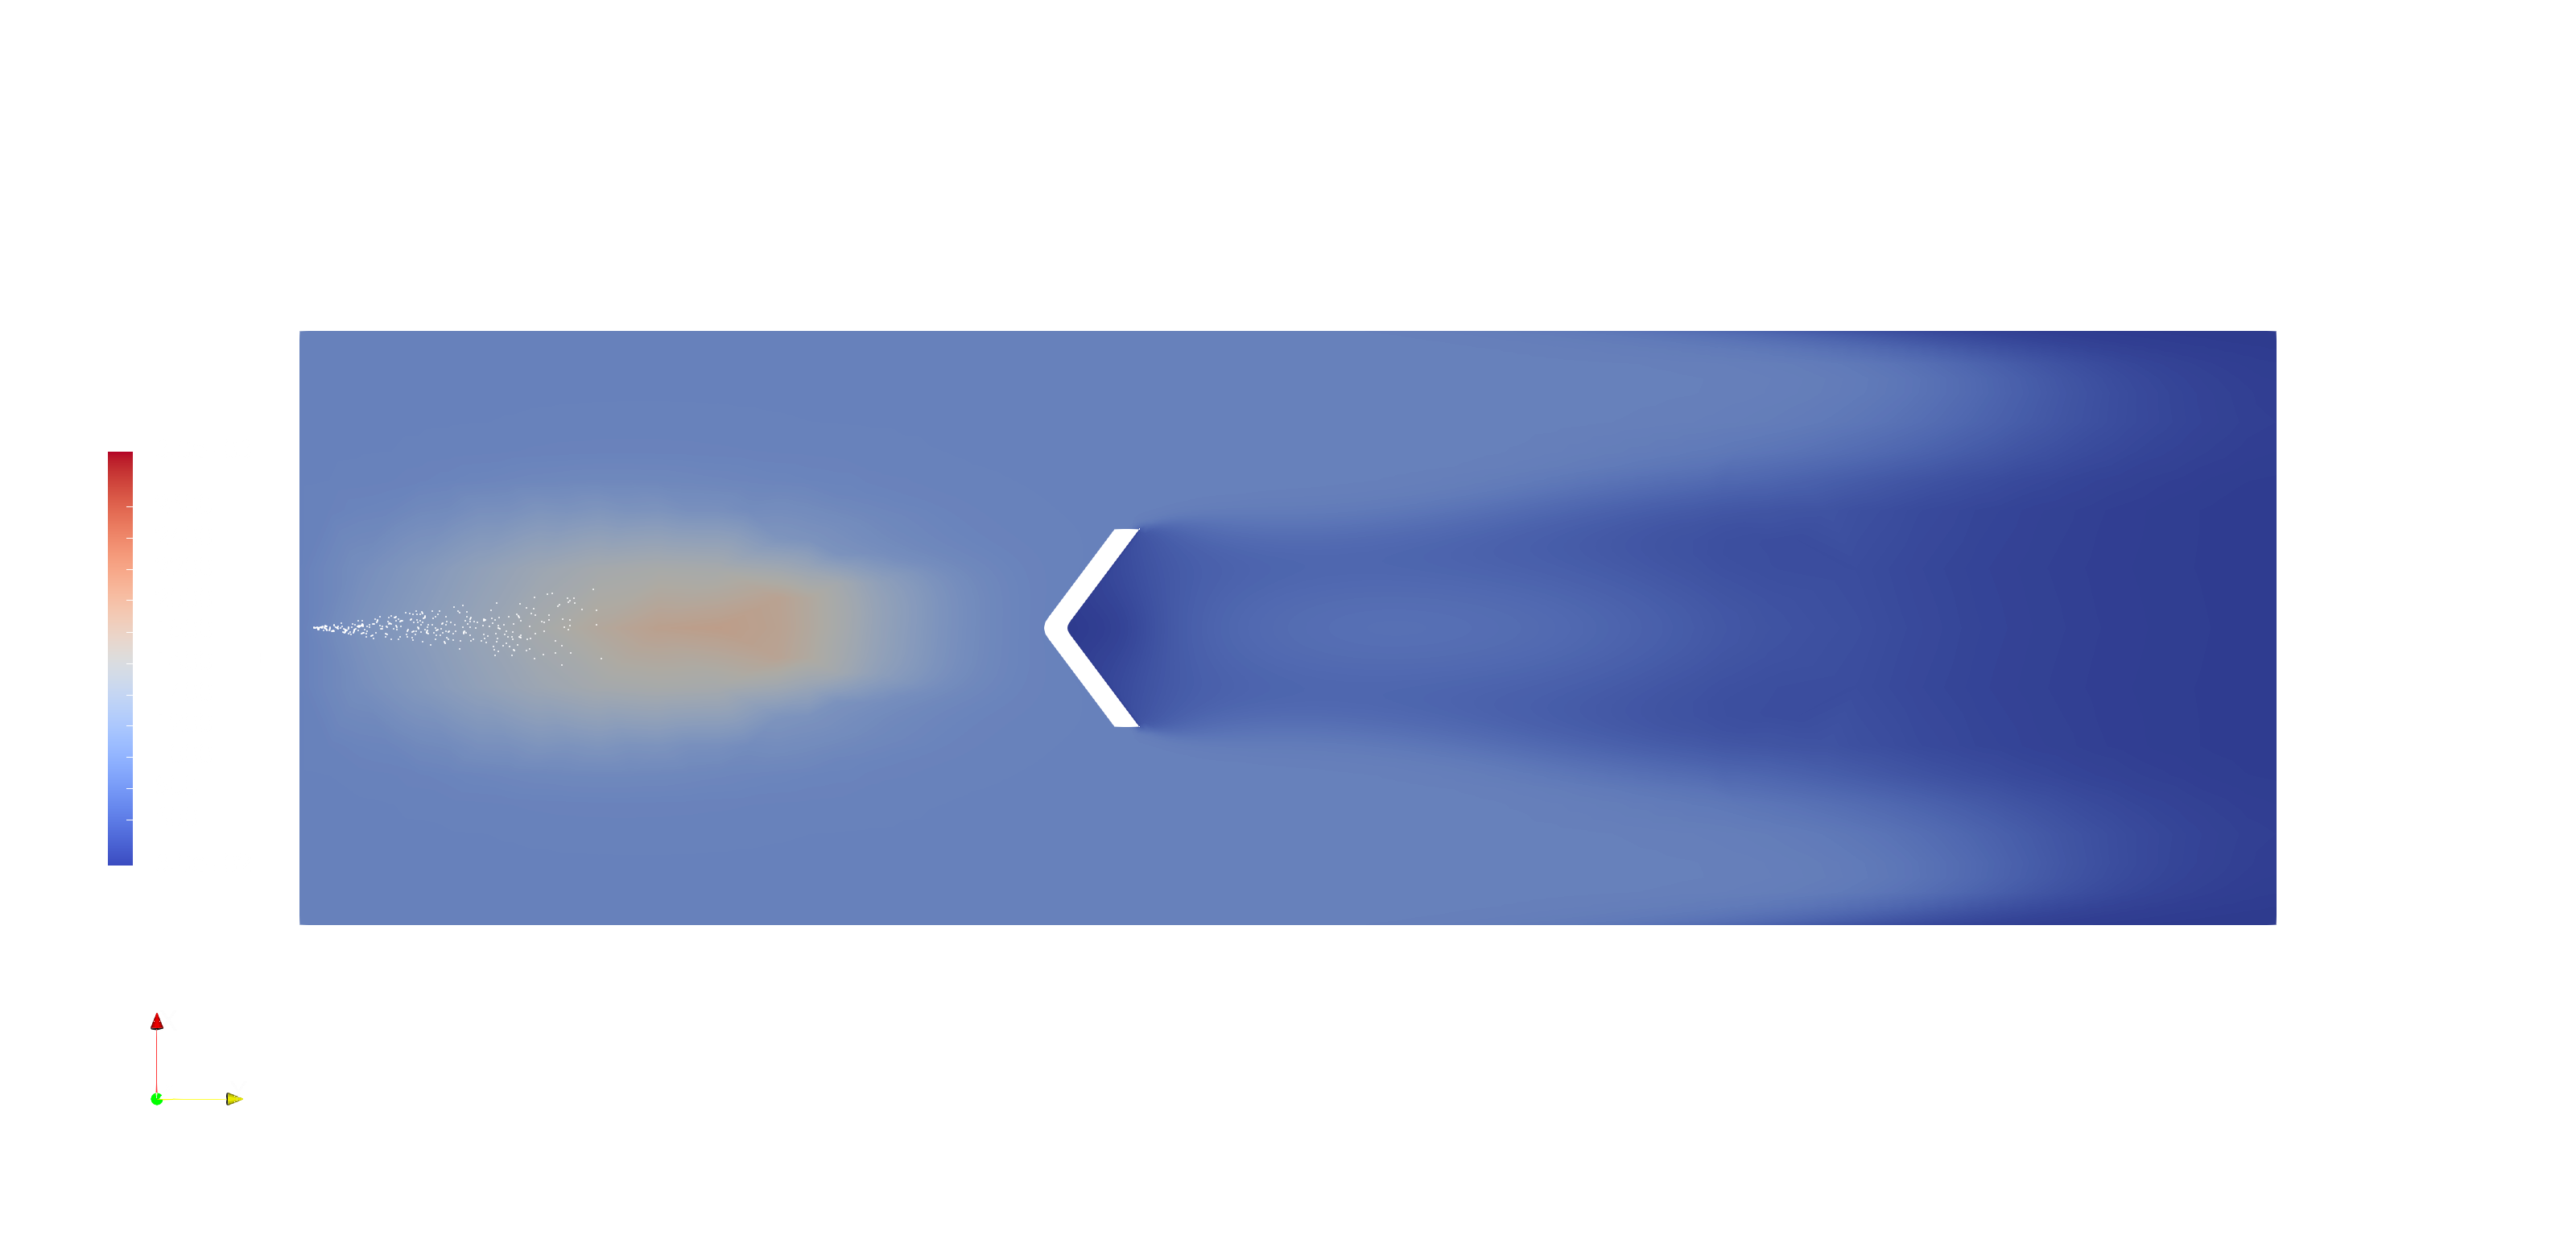
\includegraphics[width=0.8\textwidth]{latexFIGS/labAssignment/figT_02.png}
        \caption{3D reaction case: $T$ profile, $t = 0.02s$.}
    \end{figure}
    
    \begin{figure}[!ht]
        \centering
        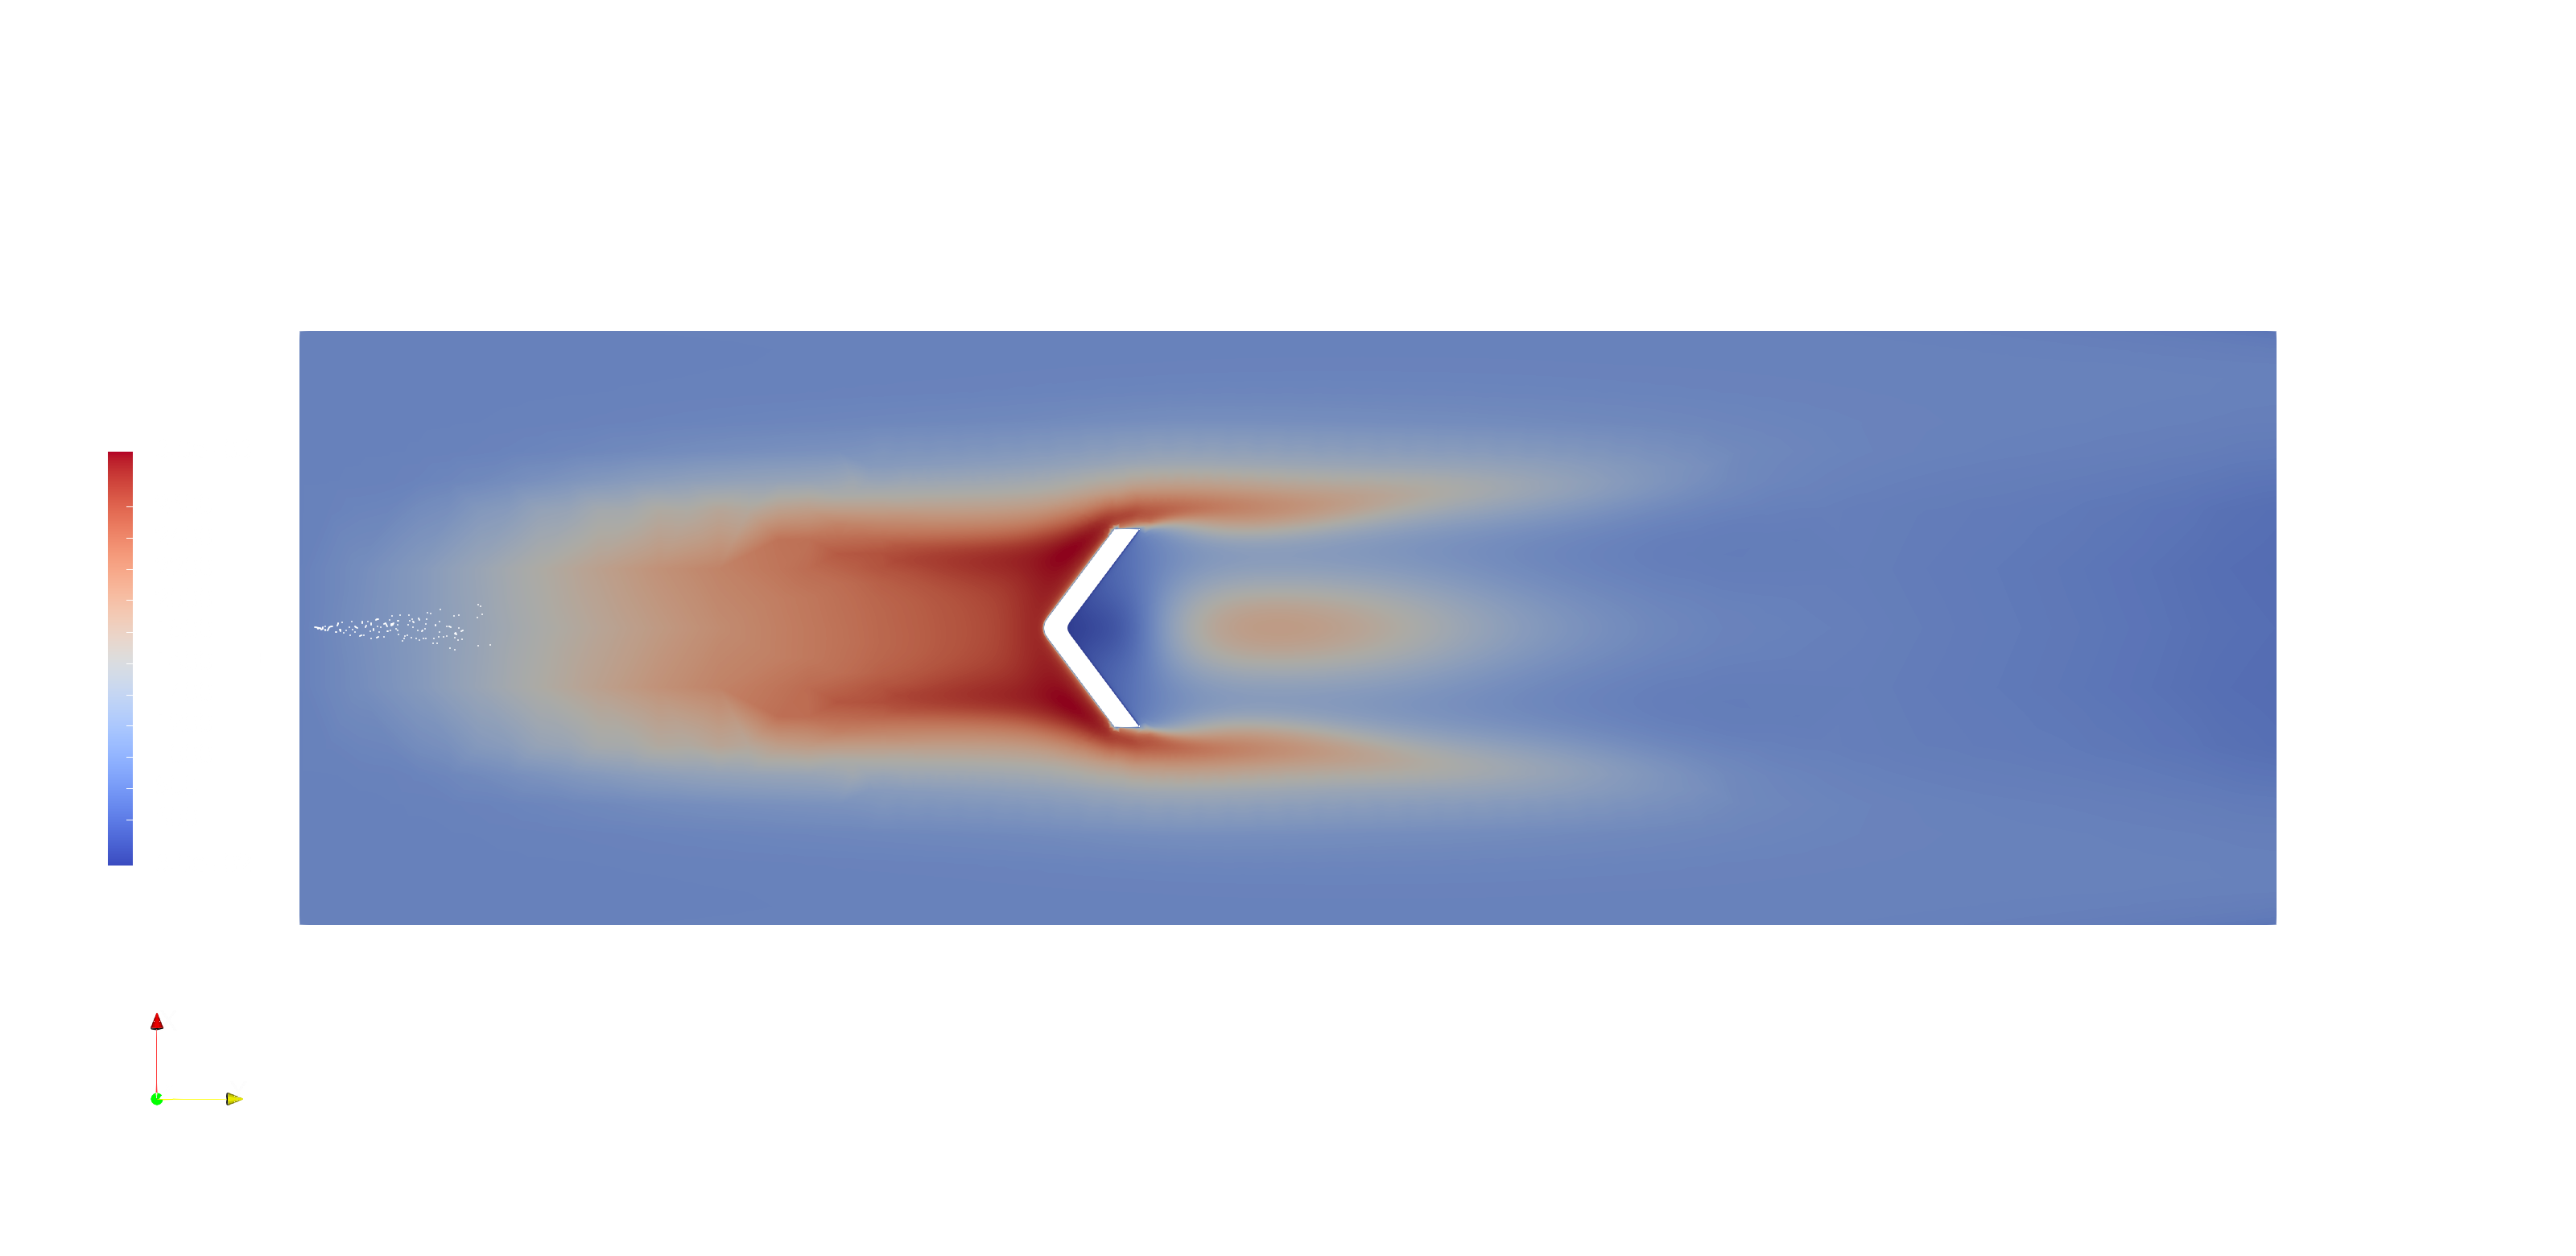
\includegraphics[width=0.8\textwidth]{latexFIGS/labAssignment/figT_05.png}
        \caption{3D reaction case: $T$ profile, $t = 0.05s$.}
    \end{figure}

    \begin{figure}[!ht]
        \centering
        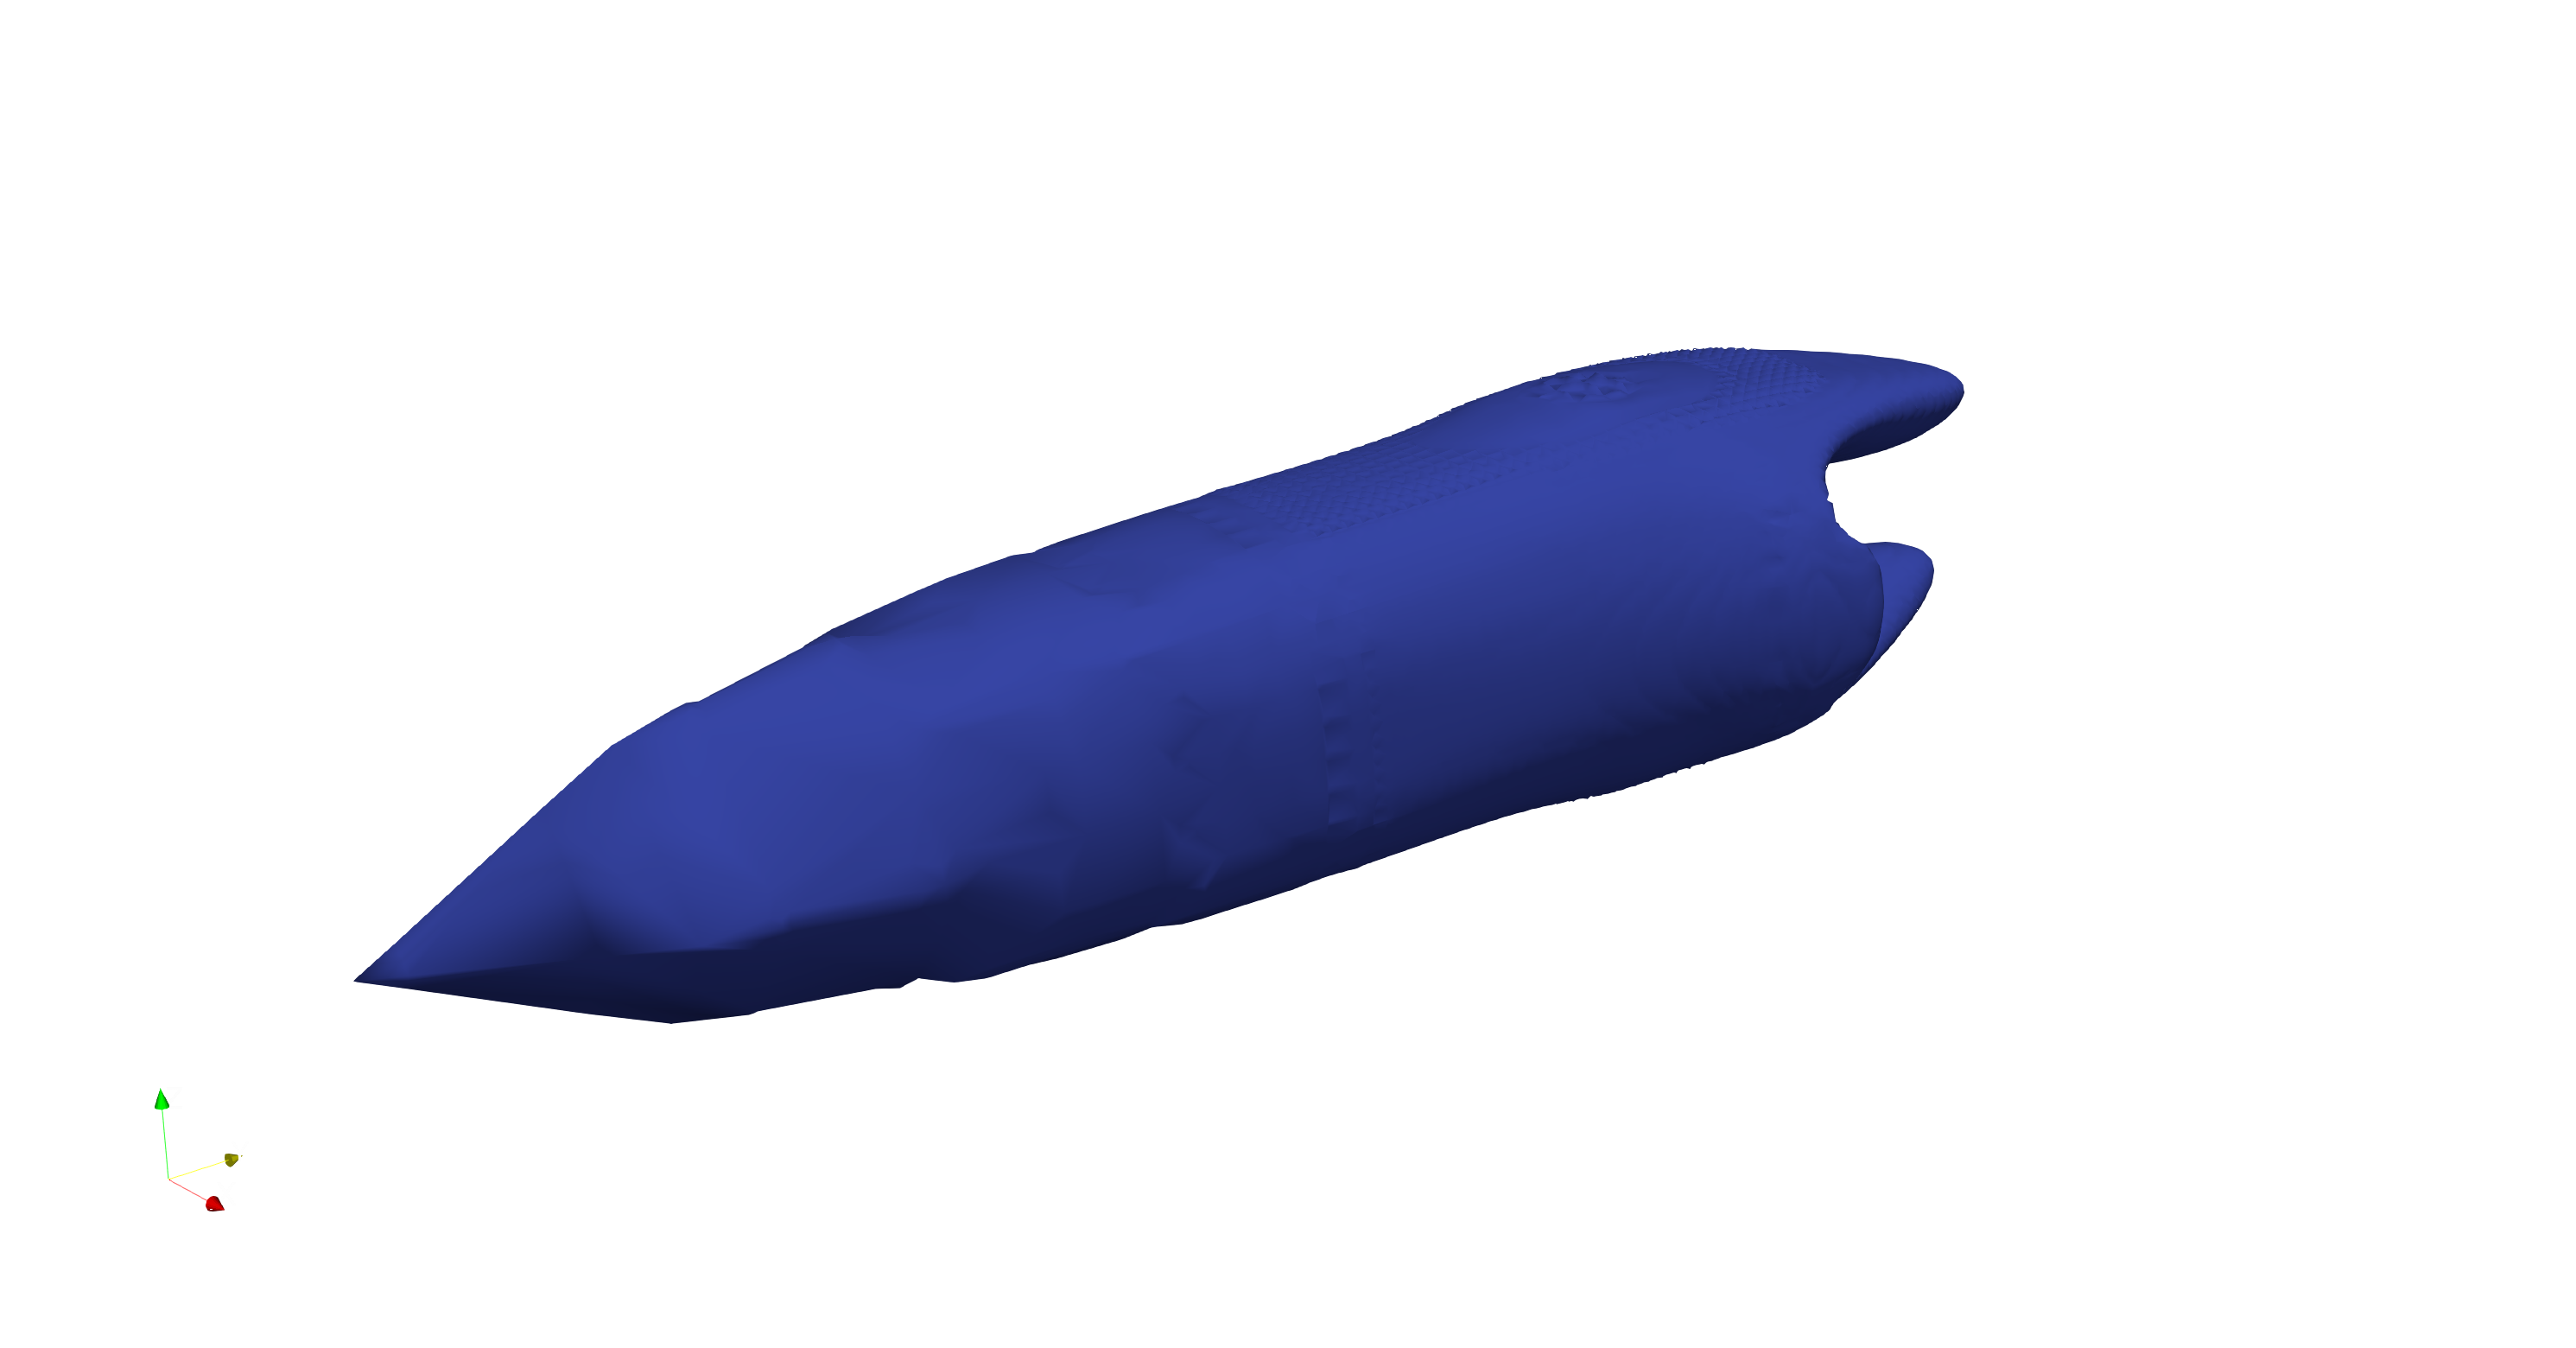
\includegraphics[width=0.8\textwidth]{latexFIGS/labAssignment/figAF.png}
        \cprotect\caption[3D reaction case: \verb|A/F| iso-surface, $t = 0.05s$]{3D reaction case: \verb|A/F| iso-surface, $t = 0.05s$. \newline ${C_7H_{16}}^{0.25} + 11 {O_2}^{1.5} \rightarrow 7 CO_2 + 8 H_2O$ \newline $\frac{A}{F} = \frac{O_2}{C_7H_{16}} \rightarrow surf\big( \frac{11 \cdot O_2^{1.5}}{{C_7H_{16}}^{0.25}} \big) = 1$}
    \end{figure}
    
    \clearpage

    
    \clearpage
    \appendix
    \addcontentsline{toc}{section}{Appendices}
    \section*{Appendices}
    \section{Mesh properties} \label{app:appMesh}

    \renewcommand{\thepage}{\arabic{page}}
    \setcounter{page}{\thelastPage}

\subsection{Non orthogonality} \label{sec:nonOrtho}
    The non orthogonality is a mesh \textbf{property} (Figure~\ref{fig:nonOrtho}) based on the \textit{vectorial} difference between the face normal versor $\boldsymbol{n}$ - at face middle point $P$ - and the versor between the control volume and its neighbour cell, $\overline{C_1 C_2}$. This property is expressed through $\theta_{no}$: the closer to $0$ the better. The non orthogonality importance is related to the \verb|FVM| that bases the fluxes computation on vector $\boldsymbol{n}$. 

\definecolor{qqwuqq}{rgb}{0,0.39,0}
\definecolor{ffqqqq}{rgb}{1,0,0}
\definecolor{qqqqff}{rgb}{0,0,1}
\definecolor{qqttff}{rgb}{0,0.2,1}
\definecolor{zzttqq}{rgb}{0.6,0.2,0}
\definecolor{cqcqcq}{rgb}{0.75,0.75,0.75}
\begin{figure}[h!]
    \centering
\begin{tikzpicture}[line cap=round,line join=round,x=1.5cm,y=1.5cm]
%\draw [color=cqcqcq,dash pattern=on 1pt off 1pt, xstep=0.5cm,ystep=0.5cm] (-0.1,-0.1) grid (5.3,3.5);
\draw[->,color=black] (-0.1,0) -- (5.3,0);
\foreach \x in {,0.5,1,1.5,2,2.5,3,3.5,4,4.5,5}
\draw[shift={(\x,0)},color=black] (0pt,2pt) -- (0pt,-2pt) node[below] {\footnotesize $\x$};
\draw[->,color=black] (0,-0.1) -- (0,3.5);
\foreach \y in {,0.5,1,1.5,2,2.5,3}
\draw[shift={(0,\y)},color=black] (2pt,0pt) -- (-2pt,0pt) node[left] {\footnotesize $\y$};
\draw[color=black] (0pt,-10pt) node[right] {\footnotesize $0$};
\clip(-0.1,-0.1) rectangle (5.3,3.5);
\fill[color=zzttqq,fill=zzttqq,fill opacity=0.1] (0,3) -- (0,0) -- (3,0) -- (2,3) -- cycle;
\fill[color=qqttff,fill=qqttff,fill opacity=0.1] (2,3) -- (3,0) -- (5,0) -- (5,3) -- cycle;
\draw [shift={(2.5,1.5)},color=qqwuqq,fill=qqwuqq,fill opacity=0.1] (0,0) -- (0:0.44) arc (0:18.43:0.44) -- cycle;
\draw (0,3)-- (0,0);
\draw (3,0)-- (0,0);
\draw (3,0)-- (2,3);
\draw (2,3)-- (0,3);
\draw (2,3)-- (5,3);
\draw (5,3)-- (5,0);
\draw (3,0)-- (5,0);
\draw [color=zzttqq] (0,3)-- (0,0);
\draw [color=zzttqq] (0,0)-- (3,0);
\draw [color=zzttqq] (3,0)-- (2,3);
\draw [color=zzttqq] (2,3)-- (0,3);
\draw [color=qqttff] (2,3)-- (3,0);
\draw [color=qqttff] (3,0)-- (5,0);
\draw [color=qqttff] (5,0)-- (5,3);
\draw [color=qqttff] (5,3)-- (2,3);
\draw (1.5,1.5)-- (3.5,1.5);
\draw [->] (2.5,1.5) -- (3.45,1.82);
\begin{scriptsize}
\fill [color=black] (0,3) circle (2.0pt);
\fill [color=black] (0,0) circle (2.0pt);
\fill [color=black] (3,0) circle (2.0pt);
\fill [color=black] (2,3) circle (2.0pt);
\fill [color=black] (5,3) circle (2.0pt);
\fill [color=black] (5,0) circle (2.0pt);
\fill [color=qqqqff] (1.5,1.5) circle (2.5pt);
\draw[color=qqqqff] (1.4,1.3) node {$C_1$};
\fill [color=qqqqff] (3.5,1.5) circle (2.5pt);
\draw[color=qqqqff] (3.5,1.3) node {$C_2$};
\fill [color=ffqqqq] (2.5,1.5) circle (2.5pt);
\draw[color=ffqqqq] (2.43,1.34) node {$P$};
\draw[color=black] (3.05,1.8) node {$n$};
\draw[color=qqwuqq] (2.97,1.37) node {$\theta_{no}$};
\end{scriptsize}
\end{tikzpicture}
    \caption{Non orthogonality.}
    \label{fig:nonOrtho}
\end{figure}


There are many correctors for this topologic issue that are related on flux corrections. One of the main numeric operator that suffers a lot of bad non orthogonality values is the laplacian, $\boldsymbol{\Delta}$. One of the most important equation related to $\boldsymbol{\Delta}$ is the \textbf{Helmolts} equation - \textbf{Poisson} equation in the incompressible cases - that is about mass conservation (one of the most important principles to satisfy). Good non orthogonality values (in OpenFOAM syntax) are: $75 - 80$.

\subsection{Skewness} \label{sec:skewness}
As the non orthogonality, the skewness is a mesh \textbf{property} (Figure~\ref{fig:skewness}). This property is extremelly dependent on mesh topology and it has a very important effect on the simulation. This property is based on the computation of a quantity at face center. To compute this quantity, the \verb|FVM| uses an interpolatory scheme that is based on control volumes' center distances. If the approximation of the field - and then the interpolation of fluxes at face center based on this field - is wrong, the whole simulation will suffer of sources/sinks like presence in the domain that will bring to errors in the results and also to having bad effects on covergence rates. 
    
\begin{figure}[h!]
    \centering
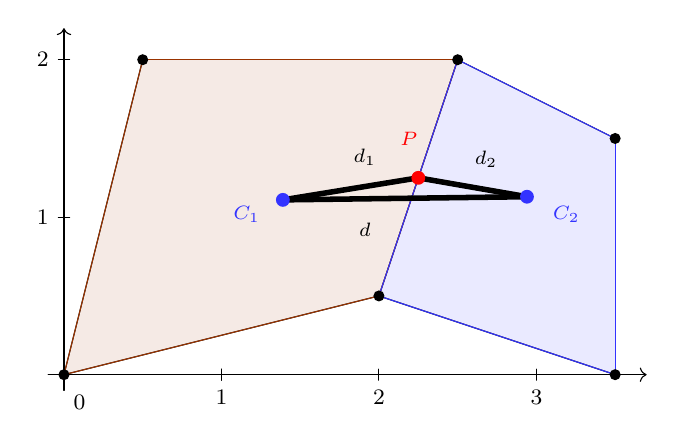
\begin{tikzpicture}[line cap=round,line join=round,x=2cm,y=2cm]
%\draw [color=cqcqcq,dash pattern=on 1pt off 1pt, xstep=1.5cm,ystep=1.5cm] (-0.1,-0.1) grid (3.7,2.2);
\draw[->,color=black] (-0.1,0) -- (3.7,0);
\foreach \x in {,1,2,3}
\draw[shift={(\x,0)},color=black] (0pt,2pt) -- (0pt,-2pt) node[below] {\footnotesize $\x$};
\draw[->,color=black] (0,-0.1) -- (0,2.2);
\foreach \y in {,1,2}
\draw[shift={(0,\y)},color=black] (2pt,0pt) -- (-2pt,0pt) node[left] {\footnotesize $\y$};
\draw[color=black] (0pt,-10pt) node[right] {\footnotesize $0$};
\clip(-0.1,-0.1) rectangle (3.7,2.2);
\fill[color=zzttqq,fill=zzttqq,fill opacity=0.1] (0.5,2) -- (0,0) -- (2,0.5) -- (2.5,2) -- cycle;
\fill[color=ttttff,fill=ttttff,fill opacity=0.1] (2,0.5) -- (3.5,0) -- (3.5,1.5) -- (2.5,2) -- cycle;
\draw (0.5,2)-- (0,0);
\draw (0,0)-- (2,0.5);
\draw (2,0.5)-- (3.5,0);
\draw (3.5,0)-- (3.5,1.5);
\draw (0.5,2)-- (2.5,2);
\draw (2.5,2)-- (3.5,1.5);
\draw (2.5,2)-- (2,0.5);
\draw [color=zzttqq] (0.5,2)-- (0,0);
\draw [color=zzttqq] (0,0)-- (2,0.5);
\draw [color=zzttqq] (2,0.5)-- (2.5,2);
\draw [color=zzttqq] (2.5,2)-- (0.5,2);
\draw [color=ttttff] (2,0.5)-- (3.5,0);
\draw [color=ttttff] (3.5,0)-- (3.5,1.5);
\draw [color=ttttff] (3.5,1.5)-- (2.5,2);
\draw [color=ttttff] (2.5,2)-- (2,0.5);
\draw [line width=2pt] (1.39,1.11)-- (2.94,1.13);
\draw [line width=2pt] (1.39,1.11)-- (2.25,1.25);
\draw [line width=2pt] (2.25,1.25)-- (2.94,1.13);
\begin{scriptsize}
\fill [color=black] (0.5,2) circle (2.0pt);
\fill [color=black] (0,0) circle (2.0pt);
\fill [color=black] (2,0.5) circle (2.0pt);
\fill [color=black] (2.5,2) circle (2.0pt);
\fill [color=black] (3.5,0) circle (2.0pt);
\fill [color=black] (3.5,1.5) circle (2.0pt);
\fill [color=ffqqqq] (2.25,1.25) circle (2.5pt);
\draw[color=ffqqqq] (2.19,1.5) node {$P$};
\fill [color=ttttff] (1.39,1.11) circle (2.5pt);
\draw[color=ttttff] (1.16,1.02) node {$C_1$};
\fill [color=ttttff] (2.94,1.13) circle (2.5pt);
\draw[color=ttttff] (3.19,1.02) node {$C_2$};
\draw[color=black] (1.91,0.92) node {$d$};
\draw[color=black] (1.91,1.38) node {$d_1$};
\draw[color=black] (2.68,1.37) node {$d_2$};
\end{scriptsize}
\end{tikzpicture}
    \caption{Skewness.}
    \label{fig:skewness}
\end{figure}


In contrast to the non orthogonality property, this property cannot be numerically \textbf{fixed}. As consequence, it is necessary to have meshes with the lowest skewness possible. It can happen that bad skewness brings to remeshing all the domain. Good skewness values (in OpenFOAM syntax) are: $1 - 8$. 

    \newpage
    \section{Incompressible solvers properties} \label{app:app1}
\subsection{$t$ discretization in OpenFOAM}
In \verb|PISO/PIMPLE| the time advancing is made in order to discretize the time derivative. As result, the $t$ advancing in the \verb|PISO/PIMPLE| solver has a physical meaning. The contrary is for the \verb|SIMPLE| solver where, in the \verb|fvSchemes|, the time discretization is absent (Listing~\ref{list:ddtSchemes}). In \verb|SIMPLE|, the $t$ advancement is essentially a controller for an additional loop over the predictor-corrector steps. As result, the previous step gives us a better estimate of $p^* - \boldsymbol{u}^*$ used for the numerical problem assembly.

\begin{lstlisting}[caption = $\mathtt{combustorSimple/system/fvSchemes}$ time discretization., label = list:ddtSchemes]
    ddtSchemes  // time derivative discretization 
        {       // no need of temporal discretization in SIMPLE algorithm
            default steadyState; // => no time stencil 
        }
    \end{lstlisting}

\cprotect\subsection{\verb|PISO| vs \verb|PIMPLE|}
The main difference between these two models consists in the \textbf{outer} correction. \verb|PISO| does not have outer correctors. The outer corrector loop consists in a correction of $p^* - \boldsymbol{u}^*$ used in the predictor step\cprotect\footnote{Solved if \verb|momentumPredictor yes;| in \verb|applications/solvers/incompressible/simpleFoam| with check on \verb|simple.momentumPredictor()|.}. This allows, relating all the process to the $\boldsymbol{u}$ at the previous outer corrector step, to find a much more correct estimate of $\boldsymbol{u}$ at the new time step due to the fact that we have a better system formulation (based on $p - \boldsymbol{u}$ already estimated at the end of the previous predictor-corrector steps) that makes the problem treatment much like an \textbf{implicit} method. The \textbf{outer} correction step is very computational demanding but, at the same time, it is possible using $\Delta t$ such that $Co > 1$. So choosing between \verb|PISO| and \verb|PIMPLE|, other than convergence and numerics, can be described with time step iterations\cprotect\footnote{It is important to keep in mind that \verb|pisoFoam| in OpenFOAM does not change the $\Delta t$. In order to solve this issue - so keeping $Co < 1$ and allowing $\Delta t$ to change -, it is used running \verb|pimpleFoam| in \verb|PISO| mode. Of course, the number of outer corrector for \verb|pimpleFoam| in \verb|PISO| mode is $0$.}.  

\subsubsection{Courant-Friedrichs-Lewy} 
In time marching problems, the CFL test allows to find a proper time step in order to link the \textbf{spatial} stencil with the \textbf{temporal} stencil, Figure~\ref{fig:CFL}.

\begin{figure}[h!]
\vspace*{-1.5cm}
\centering
\definecolor{ttttff}{rgb}{0.2,0.2,1}
\definecolor{qqqqff}{rgb}{0,0,1}
\begin{tikzpicture}[line cap=round,line join=round,x=1cm,y=1cm]
\draw[->,color=black] (1,0) -- (7,0);
\foreach \x in {1,2,3,4,5,6,7}
\draw[->,color=black] (1,-0.1) -- (1,2);
\draw[shift={(1,0)},color=black] (2pt,0pt) -- (-2pt,0pt) node[left] {\footnotesize ${t}$};
\draw[shift={(1,1)},color=black] (2pt,0pt) -- (-2pt,0pt) node[left] {\footnotesize $t + \Delta t$};
\clip(0.9,-0.89) rectangle (7,3.57);
\draw [line width=2pt,dash pattern=on 1pt off 1pt,domain=-0.37:7.9] plot(\x,{(--4-0*\x)/4});
\draw [line width=2pt] (2,0)-- (4,0);
\draw [line width=2pt] (4,0)-- (6,0);
\draw [line width=1.2pt,dotted] (2,0)-- (4,1);
\draw [line width=1.2pt,dotted] (4,1)-- (6,0);
\draw [line width=1.2pt,color=ttttff] (4,1)-- (4.82,0);
\draw [line width=1.2pt,color=ttttff] (4,1)-- (2.83,0);
\begin{scriptsize}
\fill [color=black] (2,0) circle (2pt);
    \draw[color=black] (2.2,-0.1) node[below] {$x_{(t)} - \Delta x_{(t)}$};
\fill [color=black] (4,0) circle (2pt);
    \draw[color=black] (4.09,-0.09) node[below] {$x_{(t)}$};
\fill [color=black] (6,0) circle (2pt);
    \draw[color=black] (6.21,-0.1) node[below] {$x_{(t)} + \Delta x_{(t)}$};
\fill [color=qqqqff] (4,1) circle (2pt);
    \draw[color=qqqqff] (4.26,1.12) node[above] {$x_{(t + \Delta t)}$};
\end{scriptsize}
\end{tikzpicture}
    
    \caption{CFL, spatial and temporal stencils.}
    \label{fig:CFL}

\end{figure}


As result, it is ensured that the $p - \boldsymbol{u}$ fields are physically related to the previous time steps. Of course, using $Co < 1$ does not guarantee achieving convergence; the convergence is related also to the discretization schemes and the correctors - so mainly, how the problem is solved -. The CFL condition is expressed as \cite[Ch. 13]{quarteroni2012numerical}:

\begin{equation}
    max_{\Omega} \Bigg( \frac{\big| \boldsymbol{u} \big| \ \Delta t}{\Delta x} \Bigg) < 1.0
    \label{eqn:CFL}
\end{equation}

\noindent From (\ref{eqn:CFL}), $\Delta t$ is computed. There are methods, such as \verb|PIMPLE|, that allow relaxation on this stencils constraint; this is mainly related to the way the solution is computed. $Co > 1$ acts as a filter on the solution: physics with time scales shorter than $\Delta t$ are not seen in the final solution e.g. vortex shedding. In addition, for $Co > 1$ the time discretization error propagates on the solution; the last time step is the initial condition for the new time step. In OpenFOAM the Courant-Friedrichs-Lewy conditions is expressed through \verb|maxCo|. 

\subsection{Under relaxation}
The under relaxation consists in changing the value of a computed field in order to smooth out convergence. The under relaxation process followed in many codes is the \textbf{Patankar} model~\cite[Ch. 14.1]{moukalled2016finite}, that consists in an explicit (\ref{eqn:expPATANKAR}) and an implicit (\ref{eqn:PATANKAR}) formulation:
\begin{align}
    \phi_{j + 1}^{relaxed} & = \phi_{j} + \alpha_{\phi} \ \big( \phi_{j + 1} - \phi_{j} \big) \label{eqn:expPATANKAR} \\ 
    \frac{a_C}{\lambda_{\phi}} \ \phi_{C_{j + 1}} + \sum_F a_F \ \phi_{F_{j + 1}} & = b_C + \frac{1 - \lambda_{\phi}}{\lambda_{\phi}} \ a_C \ \phi_{C_j} 
    \label{eqn:PATANKAR}
\end{align}

\noindent This model relies on $\alpha_{\phi}$ that is the relaxation parameter of the $\phi$ field. The most used $\alpha_{\phi}$ values are: $\alpha_{\boldsymbol{u}} \approx 0.7$ and $\alpha_{p} \approx 0.3$. Now, having explained the relaxation model, it is necessary to relate it to the different algorithms. The under relaxation is not present in the \verb|PISO| algorithm; this because the under relaxed field without outer corrector loop generates a not physical field, so it should not became an output of the solver. As this said, the \verb|PISO| algorithm outputs directly the $p$ field and the corrected $\boldsymbol{u}$ field ($\boldsymbol{u} = \boldsymbol{u}_{(p, \ \boldsymbol{u}^*)}$). The other algorithms, \verb|SIMPLE| and \verb|PIMPLE|, allow using under relaxation. The under relaxation parameters are expressed in \verb|system/fvSolution| with \verb|relaxationFactors| and it can be explicit on a field with \verb|fields| setting or implicit in the equations with \verb|equations| setting.

    \newpage
    \section{Compressible solvers properties} \label{app:app2}
\subsection{Energy equation}
With respect to the incompressible case, the compressible case enables the changes in $\rho$ of the fluid. This new degree of freedom in the system has to be treated with care using the energy equation. The energy equation has different forms that suit best for defined physical behaviours in the system\footnote{$h$ is the specific enthalpy, $e$ is the specific internal energy, $K$ is the total kinetic energy and $E$ is the total energy.}:

{\small
\begin{align} 
    \frac{\partial \rho e}{\partial t} + \boldsymbol{\nabla} \cdot \big( \rho \boldsymbol{u} e \big) + \frac{\partial \rho K}{\partial t} + \boldsymbol{\nabla} \cdot \big( \rho \boldsymbol{u} K \big) + \boldsymbol{\nabla} \cdot \big( \boldsymbol{u} p \big) = - \boldsymbol{\nabla} \cdot \boldsymbol{q} + \boldsymbol{\nabla} \cdot \big( \boldsymbol{\tau} \cdot \boldsymbol{u} \big) + \rho r + \rho \boldsymbol{g} \cdot \boldsymbol{u} \label{eqn:heqn} \\  
    \frac{\partial \rho h}{\partial t} + \boldsymbol{\nabla} \cdot \big( \rho \boldsymbol{u} h \big) + \frac{\partial \rho K}{\partial t} + \boldsymbol{\nabla} \cdot \big( \rho \boldsymbol{u} K \big) - \frac{\partial p}{\partial t} = - \boldsymbol{\nabla} \cdot \boldsymbol{q} + \boldsymbol{\nabla} \cdot \big( \boldsymbol{\tau} \cdot \boldsymbol{u} \big) + \rho r + \rho \boldsymbol{g} \cdot \boldsymbol{u} \label{eqn:eeqn} \\  
    \frac{\partial \rho E}{\partial t} + \boldsymbol{\nabla} \cdot \big( \rho \boldsymbol{u} E \big) + \boldsymbol{\nabla} \cdot \big( \boldsymbol{u} p \big) = - \boldsymbol{\nabla} \cdot \boldsymbol{q} + \boldsymbol{\nabla} \cdot \big( \boldsymbol{\tau} \cdot \boldsymbol{u} \big) + \rho r + \rho \boldsymbol{g} \cdot \boldsymbol{u} \label{eqn:Eeqn}  
\end{align}. 
}

One of the most used energy equation is in the $h$ formulation~\cite[Ch. 11]{ferziger2002computational}. The $h$ formulation uses $h = e + \frac{p}{\rho}$ and $K$ as \textit{thermodynamic} and \textit{mechanical} energy describers. In both $h - e$ formulations, $K$ is always computed; instead in the total energy formulation, $K$ is hidden in $E = e + K$. Most of the energy formulations in OpenFOAM neglect the mechanical part $\boldsymbol{\nabla} \cdot \big( \boldsymbol{\tau} \cdot \boldsymbol{u} \big)$ and $\rho \boldsymbol{g} \cdot \boldsymbol{u}$.  

In the whole assignment, the compressibility is treated with the $h$ formulation. The reason about this choice relies on the physics of the problem: for a problem with heat flux and with combustion of a non premixed mixture, the $h$ formulation is preferred.

\subsubsection{$h$ equation in OpenFOAM}
There are different ways for solving the compressible flow problems. The philosophy stays the same. One of the possible $h$ formulations is described in \verb|rhoPimpleFoam| and the main codes used in it are \verb|pEqn.H|, \verb|UEqn.H|, \verb|EEqn.H| and \verb|rhoPimpleFoam.C|. 

The main parts of \verb|rhoPimpleFoam.C| are the following: 
\begin{itemize}
    \item \textbf{Outer loop}
    \begin{itemize}
        \item \textbf{$\rho$ computation} - \verb|rhoEqn.H| - Since $\rho$ is a derived field, it needs to be computed. 
        \item \textbf{$\boldsymbol{u}$ predictor} - \verb|UEqn.H| - Computation of a first $\boldsymbol{u}$ approximation. 
        \item \textbf{$h$ equation} - \verb|EEqn.H|\cprotect\footnote{\verb|EEqn.H| uses \verb|dpdt|. \verb|dpdt| is computed in \verb|pEqn.H| with \verb|dpdt = fvc::ddt(p)|.} - Computation of the $h - T$ field through guessed $\rho - p^*$ and the previous predicted $\boldsymbol{u}$. 
        \item \textbf{Inner loop}
        \begin{itemize}
            \item \textbf{$p$ corrector} - \verb|pEqn.H|\cprotect\footnote{The Helmoltz equation can be seen as a Poisson equation with a $\frac{\partial \rho}{\partial t}$ term that is converted in $p$ terms and then treated implicitly.} - Guarantee continuity with Helmolts equation.
            \begin{itemize}
                \item \textbf{$\frac{\partial p}{\partial t}$ computation} Computation of $\frac{\partial p}{\partial t}$ needed in $h$ formulation.
            \end{itemize}
            \item \textbf{$\rho$ computation/correction} - \verb|rhoEqn.H| - Correcting again $\rho$ field with new $p$ field and the $T$ field from the $h$ equation solution.
    \end{itemize}
    \end{itemize}
    \item \textbf{Convergence check}
    \item \textbf{Time step advancement}
    \begin{itemize}
        \item \textbf{Guessed fields for the new time step} The new time step gets the guessed values from the last time step solutions.
    \end{itemize}
\end{itemize}

\subsubsection{$\psi$ and $\rho$ based model}
In CFD there are many ways for coupling the energy, pressure, velocity equations and the equation of state. All these ways for the computation of $\rho$ can be separated in 2 families: the pressure based $\psi$ equation and the $\rho$ based equations. 

\paragraph{$\psi$} The $\psi$ based equations uses an explicit relation between $\rho$ and $p$ through $\psi$. An example is the $\psi$ equation that is based on the equation of the perfect gases, $\psi = \frac{1}{R T}$ such that $\rho = \psi \cdot p$. This family of models are best suitable for the segregated (semi-implicit) method because it is a \textbf{$p$ based} algorithm.

\paragraph{$\rho$} The $\rho$ based equations are another set of equations that allow the computation of $\rho$ through a $\rho$ dependent PDE or through an equation that does not explicitly relate $\rho$ to $p$ such as the \textbf{Boussinesque approximation} $\Delta \rho = \beta \Delta T$.

    \newpage
    \section{Spray modeling} \label{app:app3_1}
    \subsection{Spray regions description}
    Sprays are largely used in the combustion field. The aim is to let the fuel evaporate in the shortest time possible to reach the best performances.
    Engineers have divided the spray in 3 regions and one of the main describers can be the void fraction\footnote{$\alpha = \frac{V_{liquid}}{V_{cell}}$}: 
    \begin{itemize}
        \item \textbf{Dense region} In this region, there is the first break up of the jet core in many string shaped drops. The fuel has a low surface to volume ratio, this implies the fuel is a dense and confined region in the system. This region has to be treated with care and it is very computationally demanding. The models required to solve this region are called \textbf{continuous phase models}, \verb|CPM|. The void fraction for this region is around unity. 
      
        \item \textbf{Diluted region} In this region, the dense region starts to break up into smaller pieces; these pieces have a larger surface to volume ratio but not high enough to be modelled as spheric particles. This region is very important to lagrangian particles tracking methods because it is the region of transition between dense to dispersed region. This region can be treated as well with \verb|CPM|. The final aim of the \verb|CPM| in this case is to get a good description of the spray properties for the dispersed region modeling. The void fraction is around $0.5$ - this because $\frac{V_{liquid}}{V_{gas}} \approx 1$.
       
        \item \textbf{Dispersed region} This region consists of many dispersed particles where the surface to volume ratio is high enough to consider these particles as spheres. This \textbf{huge} simplification allows using the lagragian spray method for the modeling of the development of the spray in the dispersed region\cprotect\footnote{It is possible to model the dispersed region with \verb|CPM|. Using \verb|CPM| in the dispersed region means not considering the particles as spheres. \verb|CPM| in dispersed region is very computational demanding and very difficult to handle.}. In the following CFD cases, lagrangian particles models are used to discretize the spray evolution (dispersed region only) into the system. As result of dispersed fuel into the system, the void fraction is lower than $1$.
    \end{itemize}

    \subsection{Parcels in spray modeling}
    The number of particles in the dispersed region can be of order of billions; this will bring a lot of computational effort to model all the particles into the system and also to store all the data related to particles' properties, position and dynamics. In order to solve this problem, lagrangian sprays adopted a new way of modeling for these particles.
    All these particles are grouped into objects called parcels. The grouping process is related to the particles' diameter. If a particle has a certain diameter, this particle will be grouped with other particles that fall inside a defined diameter range. Particles' diameter is defined by experimental results, by results analysis of dense and diluted region simulations and by statistics. After the grouping process, every parcel in the system has defined properties. The lagrangian spray modeling will compute the parcels evolution into the system. 
    
    \subsubsection{Parcels interaction}
    Since parcels represent the properties of group of particles, the evolution of parcels represents the evolution of those particles. Parcels and gaseous flow can interact in different ways. This depends on the nature of the spray, on parcels' properties and on computational power available. It is possible to model the spray as:
    \begin{itemize}
        \item \textbf{One way coupling} The one way coupling allows only a \textit{one way talk} from the continous phase to the discrete phase. This allows to compute the parcels motion directly from the continuous phase field. Of course, parcel motion depends on the forces applied to it; these forces are computed using forces equations applied to spherical shaped particels with the help of experimental results. The forces' models depend on particles diameter - expressed through parcel object -, the particles diameter on the other hand depends on the thermodynamics (because of evaporation).
        \item \textbf{Two ways coupling} The two way coupling allows the \textit{talk back} of the discrete phase evolution to the continous phase. This happens through additional source terms in the continuous phase equations. As result, this method is more computational demanding\footnote{All the modeling aspects for the parcel's evolution are the same as the one way coupling}.
        \item \textbf{Four ways coupling} The four ways coupling accounts also to the parcels interaction. Usually this method is used when $\alpha \geq 10^{-2}$. The continuous phase treatment remains almost the same as the two ways coupling but the parcels interaction has an additional modeling step that takes into account the changes parcels make into the continuous field because their distance and also the parcels interaction as parcels agglomeration and parcels break-up.
    \end{itemize}

\newpage
\section{Wall-film modeling} \label{app:app3_2}
    The particles-wall interaction has to be treated by the simulation. This interaction is very important because it can change a lot the behaviour of the solution. Wall-film in OpenFOAM are mainly treated using these hypothesis:
    \begin{itemize}
        \item \textbf{Wall-film thickness hypthesis} The wall-will thickness is supposed to be very thin; this brings to study the liquid film evolution as a 2D problem
        \item \textbf{Particles temperature change} The temperature change of the particles impinging the wall-film is slow; this allows direct analytical time integration istead of numerical integration
        \item \textbf{Conductivity hypothesis} Since the wall-film region is a layer above the solid wall, heat is transmitted from the wall to the liquid film through conductive mechanism
        \item \textbf{Temperature limits hypothesis} Due to modeling reasons, the wall and wall-film temerature is supposed to be lower than the liquid boiling temperature
    \end{itemize}

\subsection{Mesh and boundary conditions}
    Because the wall-film region can be seen as an additional model to the usual \verb|FVM| case, a mesh has to be built in order to study the wall-film region. The only purpose of the wall-film mesh is to track the development of a 3D wall-film using a 2D mesh. The wall-film has to talk back to the \textit{global} mesh in order to set up correct boundary conditions for the main flow. As result of this modeling choices, the main parameters that describe the wall-film region are:
    \begin{itemize}
        \item $\delta$ Liquid film height. Since the mesh is 2D, the wall film height is described by $\delta$ but at the same time $\delta$ describes the presence of the liquid film on the wall-film region surface
        \item $\boldsymbol{u}$ Liquid film velocity
        \item $T$ Liquid film temperature
    \end{itemize}
    
    Transport equations~(\ref{eqn:transp}) are used for tracking these quantities:
    \begin{equation}
        \begin{cases}
            \frac{\partial \rho \delta}{\partial t}  + \boldsymbol{\nabla} \cdot \big( \rho \ \delta \ \boldsymbol{u} \big) & = \boldsymbol{S}_{\delta} \\ 
            \frac{\partial \rho \delta \boldsymbol{u} }{\partial t}  + \boldsymbol{\nabla} \cdot \big( \rho \ \delta \boldsymbol{u} \ \boldsymbol{u} \big) & = - \delta \ \boldsymbol{\nabla} p + \boldsymbol{S}_{\delta \boldsymbol{u}} \\ 
            \frac{\partial \rho \delta h }{\partial t}  + \boldsymbol{\nabla} \cdot \big( \rho \ \delta h \ \boldsymbol{u} \big) & = \boldsymbol{S}_{\delta h}
        \end{cases} \label{eqn:transp}
    \end{equation}

    \newpage
    \section{Reactions} \label{app:app4}
Before starting modeling reactions it is necessary to know the species inside the system, the possible reactions that can happen and all the parameters related to transport and diffusion of these species into the system. All these properties are mainly taken from experiments or they come from chemistry modeling (for the more complicated species). 
    
\subsection{Govering equations}
    The main changes in the governing equation are made on the continuity equation. The continuity equation expresses the conservation of mass in the system. Because the presence of reactions, it is needed to track the species' evolution in the system. The continuity equations for each species are written as:
    \begin{equation}
        \frac{\partial \rho Y_i}{\partial t} + \boldsymbol{\nabla} \cdot \big( \rho \boldsymbol{u} \ Y_i  \big) = \boldsymbol{\nabla} \cdot \big( \rho \boldsymbol{v}_i \ Y_i \big) + \dot\omega_i
    \end{equation}
    Where $Y_i$ is the mass fraction of \textit{ith} species, $\boldsymbol{v}_i$ is the \textit{ith} species diffusion velocity\footnote{$\sum_i \boldsymbol{\nabla} \cdot \big( \rho Y_i \boldsymbol{v}_i \big) = 0$, where $\boldsymbol{v}_i$ is the species velocity fluctuation, $\sum_i Y_i = 1$ and $\boldsymbol{\nabla} \cdot \big( \rho \boldsymbol{u} \big) = 0$. \newline $\sum_i \boldsymbol{\nabla} \cdot \big[ Y_i \rho \big(\boldsymbol{u} + \boldsymbol{v}_i \big) \big] = \sum_i \boldsymbol{\nabla} \cdot \big( Y_i \rho \boldsymbol{u} \big) + \sum_i \boldsymbol{\nabla} \cdot \big( Y_i \rho \boldsymbol{v}_i \big) = \boldsymbol{\nabla} \cdot \big( \rho \boldsymbol{u} \sum_i Y_i \big) + \sum_i \boldsymbol{\nabla} \cdot \big( Y_i \rho \boldsymbol{v}_i \big) = 0$.} and $\dot\omega_i$ is the \textit{ith} species production due to reactions\footnote{$\sum_i \dot\omega_i = 0$ because the reaction process does not create mass, it just \textit{moves} atoms in order to create new species, conserving mass.}. As result, $\boldsymbol{v}_i$ are new degree of freedom into the system, so it is necessary to find equations that allow to treat them. The complete equation for the $\boldsymbol{v}_i$ computation is very hard to solve\footnote{$\boldsymbol{v}_p$ equation: $\boldsymbol{\nabla}X_p = \sum_k \frac{X_p \ X_k}{\mathcal{D}_{p, k}}\big( \boldsymbol{v}_k - \boldsymbol{v}_p \big) + ( Y_p - Y_k \big) \frac{\boldsymbol{\nabla} p}{p} + \frac{\rho}{p} \ \sum_k Y_p \ Y_k \big( f_p - f_k \big)$.}, so it is necessary to simplify this equation. Possible formulations are the \textbf{Fick}'s law, equation~(\ref{eqn:fick}), and the \textbf{Hirshfelder} model, equation~(\ref{eqn:hirsh}).
        \begin{align}
            \boldsymbol{v}_i & = - \mathcal{D} \boldsymbol{\nabla} \log{Y_p} \label{eqn:fick} \\ 
            \boldsymbol{v}_i \ X_k & = \mathcal{D}_k \boldsymbol{\nabla} X_k \label{eqn:hirsh}  
        \end{align}
   All these simplified submodels imply a cost, mass conservation is not guaranteed. In order to conserve the mass, it is necessary to correct these fields through:
   \begin{itemize}
       \item Reducing the number of equations for the species from $N$ to $N-1$ using the mass conservation formula $\sum_i Y_i = 1$ for the computation of the \textit{Nth} species. This procedure can work but only if the $Y_N$ is high enough to neglect these modeling errors. 
       \item A much better solution can be achieved changing the fluctuation field $\boldsymbol{v}_k$ in order to conserve total mass for all the species.
   \end{itemize}

    For the remaining governing equations, the main changes are relative the new source terms in the energy equation\footnote{The source term sign depends on the nature of the reaction.}. The momentum equation is affected most through the $\nu_{eff} = \nu + \nu_t$ due the dependence of viscosity and turbulence characteristics on the flow composition. 

    \subsection{Chemistry}
    Having introduced the way reactions talk with the \textit{main} flow governing equations, it is necessary to study the chemistry modeling in the system. This part is essential because it allows studing:
    \begin{itemize}
        \item \textbf{Combustion presence} If the energy activation threshold is overcomed, reaction takes place.
        \item \textbf{Chemical kinetics} Allows to treat the species evolution - $\dot\omega_i$ in mass conservation equation -, control volume cell species composition - for $\nu_{eff}$ assembly in momentum equation.
        \item \textbf{Chemical thermodynamics} Allows to treat heat transfered, $h_{reac}$, in energy equation. 
    \end{itemize}
    
    Most of the chemistry models are based on the \textbf{Arrhenius} law:
    \begin{equation}
        k = B \ T_a \ e^{- \frac{E_a}{R_u \ T}} \label{eqn:arrh}
    \end{equation}

    The equation~(\ref{eqn:arrh}) is a semi-empirical law\footnote{$B$ is the Boltzman constant, $B \ T_a$ is the collision frequency and $E_a$ is the energy activation for the reaction.} and it is used to determine the chemical kinetics of a reaction like the following:
    
    \begin{equation}
        \frac{\partial [C]}{\partial t} = (k_{forward} - k_{backward})  \ [A] \ [B]; \text{\ for the reaction}\footnote{The probability of having a reaction made by the interaction of more than three species is extremelly low.} \ A + B \leftrightarrow C \label{eqn:chemKin}
    \end{equation}

    Equation~(\ref{eqn:chemKin}) is an ODE that can be solved in an implicit or explicit way. Due to stiffness of equation (\ref{eqn:chemKin}) - related to the exponential nature of $k$ - an implicit formulation allows using less timesteps to reach the \textit{main} flow time step lenght but at the same time it is more computationally expensive. On the other hand, the explicit formulation in much more direct that the implicit one but it needs more iterative steps to reach the \textit{main} flow iterative time step lenght. 
    
    As result, chemistry can be seen as a computational burden for the simulation because it is related to small time steps due to the chemistry ODE stiffness properties.

%    \section{FVM, mesh and numerics}
    \setcounter{page}{1}
    \renewcommand{\thepage}{A-\arabic{page}}
    
    The \textsc{Computational techniques for thermochemical propulsion} course aims to explain different ways for solving reactive flows. In order to do this, the \textbf{finite volume method} is used for solving these flows. This method uses different solving approaches and is stricty linked to the mathematical branches of numerics and topology and to the physical branches of fluid dynamics and chemistry. 

    \subsection{FVM}    
    In this method we treat the system using a \textbf{discretized} form of the \textbf{conservative} formulation of the Navier-Stokes equations (\ref{eqn:NS}). This \textbf{discretization} uses \textbf{control volumes} and the \textbf{conservativity} behaviour of the method is expressed studying the variation inside of the control volume of $\phi$ field with respect to its \textbf{flux} over the control volume faces. In the \textbf{Eulerian} point of view, the $\phi$ field can be described as: 
    \begin{equation}
        \frac{d}{d \ t} \int_{\Omega} \rho \ \phi \ dV + \int_{\partial \Omega} \rho \ \boldsymbol{u} \ \phi \ \cdot \ \boldsymbol{n} \ dS  = \int_{\Omega} \bar{S} \ dV 
        \label{eqn:GENformulation}
    \end{equation}
   
   \noindent Where $\bar{S}$ is a souce term, $\rho$ is the density field and $\boldsymbol{u}$ is the velocity field. The main concept used into the FVM is reducing the system field into small sized control volumes; this will result in applying the same equations (\ref{eqn:GENformulation}) to just smaller control volumes. As the number of control volume increases the field becomes more like the real field. The conservativity of the method is expressed on the fact that every volume shares the same flux with the neighbour volume, as so, the conservation of a quantity $\phi$ is conserved at least in the theoretical description of the model; practically, \textit{things are a bit different due to numerics}, \ref{sec:nonOrtho} and \ref{sec:skewness}. 
   \newline The FVM bases the $\phi$ field interpolation over the control volume \textbf{cell centers}. These points describe all the field. Every value at the cell face is made by an \textbf{interpolation} in space. There exist many interpolation schemes, each scheme is based on a \textbf{computational molecule}, Figure~\ref{fig:CPmolecule}.
    
    \begin{figure}[h!]
    \centering
%    \hspace*{-0.3cm}
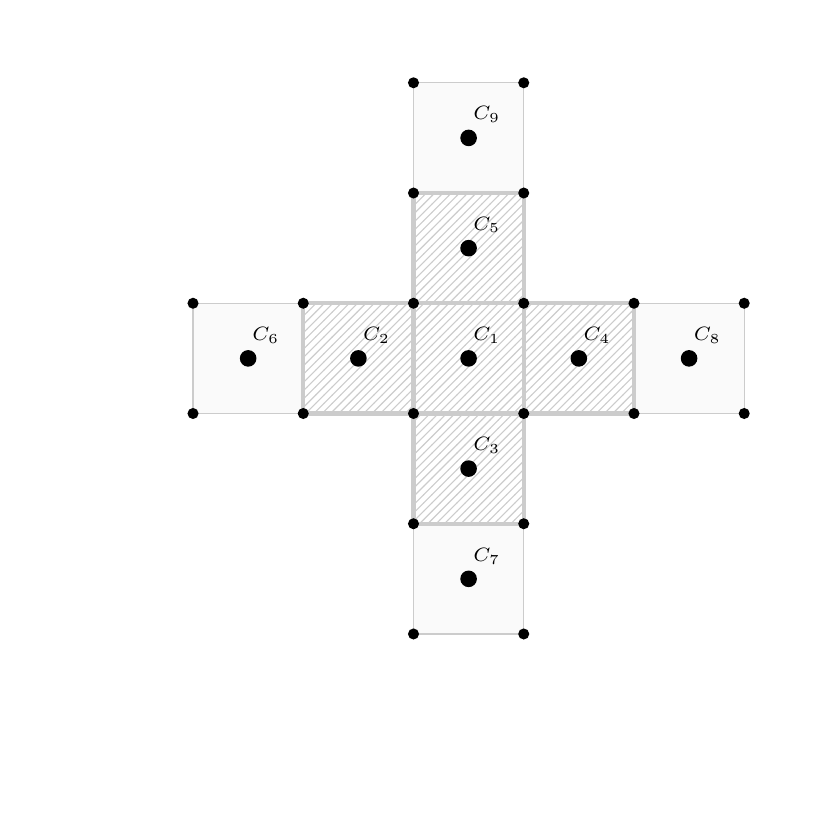
\begin{tikzpicture}[line cap=round,line join=round,x=0.7cm,y=0.7cm]
%\draw[->,color=black] (-7,0) -- (7,0);
\foreach \x in {-6,-4,-2,2,4,6}
%\draw[shift={(\x,0)},color=black] (0pt,2pt) -- (0pt,-2pt) node[below] {\footnotesize $\x$};
%\draw[->,color=black] (0,-7) -- (0,7);
\foreach \y in {-6,-4,-2,2,4,6}
%\draw[shift={(0,\y)},color=black] (2pt,0pt) -- (-2pt,0pt) node[left] {\footnotesize $\y$};
%\draw[color=black] (0pt,-10pt) node[right] {\footnotesize $0$};
\clip(-7,-7) rectangle (7,7);
\fill[color=cccccc,fill=cccccc,fill opacity=0.1] (0,6) -- (0,4) -- (2,4) -- (2,6) -- cycle;
\fill[line width=1.6pt,pattern color=cccccc,fill=cccccc,pattern=north east lines] (0,4) -- (0,2) -- (2,2) -- (2,4) -- cycle;
\fill[line width=1.6pt,pattern color=cccccc,fill=cccccc,pattern=north east lines] (-2,2) -- (-2,0) -- (0,0) -- (0,2) -- cycle;
\fill[color=cccccc,fill=cccccc,fill opacity=0.1] (-2,2) -- (-4,2) -- (-4,0) -- (-2,0) -- cycle;
\fill[line width=1.6pt,pattern color=cccccc,fill=cccccc,pattern=north east lines] (0,0) -- (2,0) -- (2,2) -- (0,2) -- cycle;
\fill[line width=1.6pt,pattern color=cccccc,fill=cccccc,pattern=north east lines] (0,0) -- (0,-2) -- (2,-2) -- (2,0) -- cycle;
\fill[color=cccccc,fill=cccccc,fill opacity=0.1] (0,-2) -- (0,-4) -- (2,-4) -- (2,-2) -- cycle;
\fill[line width=1.6pt,pattern color=cccccc,fill=cccccc,pattern=north east lines] (2,0) -- (4,0) -- (4,2) -- (2,2) -- cycle;
\fill[color=cccccc,fill=cccccc,fill opacity=0.1] (4,0) -- (6,0) -- (6,2) -- (4,2) -- cycle;
\draw (-4,2)-- (-4,0);
\draw (-4,0)-- (-2,0);
\draw (-4,2)-- (-2,2);
\draw (-2,2)-- (-2,0);
\draw (-2,0)-- (0,0);
\draw (0,0)-- (0,2);
\draw (0,2)-- (-2,2);
\draw (0,2)-- (0,4);
\draw (0,4)-- (0,6);
\draw (0,6)-- (2,6);
\draw (2,6)-- (2,4);
\draw (2,4)-- (0,4);
\draw (0,2)-- (2,2);
\draw (2,2)-- (2,4);
\draw (2,2)-- (2,0);
\draw (2,0)-- (0,0);
\draw (0,0)-- (0,-2);
\draw (0,-2)-- (0,-4);
\draw (0,-4)-- (2,-4);
\draw (2,-4)-- (2,-2);
\draw (2,-2)-- (0,-2);
\draw (2,-2)-- (2,0);
\draw (2,0)-- (4,0);
\draw (4,0)-- (4,2);
\draw (4,2)-- (2,2);
\draw (4,2)-- (6,2);
\draw (6,2)-- (6,0);
\draw (6,0)-- (4,0);
\draw [color=cccccc] (0,6)-- (0,4);
\draw [color=cccccc] (0,4)-- (2,4);
\draw [color=cccccc] (2,4)-- (2,6);
\draw [color=cccccc] (2,6)-- (0,6);
\draw [line width=1.6pt,color=cccccc] (0,4)-- (0,2);
\draw [line width=1.6pt,color=cccccc] (0,2)-- (2,2);
\draw [line width=1.6pt,color=cccccc] (2,2)-- (2,4);
\draw [line width=1.6pt,color=cccccc] (2,4)-- (0,4);
\draw [line width=1.6pt,color=cccccc] (-2,2)-- (-2,0);
\draw [line width=1.6pt,color=cccccc] (-2,0)-- (0,0);
\draw [line width=1.6pt,color=cccccc] (0,0)-- (0,2);
\draw [line width=1.6pt,color=cccccc] (0,2)-- (-2,2);
\draw [color=cccccc] (-2,2)-- (-4,2);
\draw [color=cccccc] (-4,2)-- (-4,0);
\draw [color=cccccc] (-4,0)-- (-2,0);
\draw [color=cccccc] (-2,0)-- (-2,2);
\draw [line width=1.6pt,color=cccccc] (0,0)-- (2,0);
\draw [line width=1.6pt,color=cccccc] (2,0)-- (2,2);
\draw [line width=1.6pt,color=cccccc] (2,2)-- (0,2);
\draw [line width=1.6pt,color=cccccc] (0,2)-- (0,0);
\draw [line width=1.6pt,color=cccccc] (0,0)-- (0,-2);
\draw [line width=1.6pt,color=cccccc] (0,-2)-- (2,-2);
\draw [line width=1.6pt,color=cccccc] (2,-2)-- (2,0);
\draw [line width=1.6pt,color=cccccc] (2,0)-- (0,0);
\draw [color=cccccc] (0,-2)-- (0,-4);
\draw [color=cccccc] (0,-4)-- (2,-4);
\draw [color=cccccc] (2,-4)-- (2,-2);
\draw [color=cccccc] (2,-2)-- (0,-2);
\draw [line width=1.6pt,color=cccccc] (2,0)-- (4,0);
\draw [line width=1.6pt,color=cccccc] (4,0)-- (4,2);
\draw [line width=1.6pt,color=cccccc] (4,2)-- (2,2);
\draw [line width=1.6pt,color=cccccc] (2,2)-- (2,0);
\draw [color=cccccc] (4,0)-- (6,0);
\draw [color=cccccc] (6,0)-- (6,2);
\draw [color=cccccc] (6,2)-- (4,2);
\draw [color=cccccc] (4,2)-- (4,0);
\begin{scriptsize}
\fill [color=black] (0,0) circle (2.0pt);
\fill [color=black] (2,0) circle (2.0pt);
\fill [color=black] (0,2) circle (2.0pt);
\fill [color=black] (2,2) circle (2.0pt);
\fill [color=black] (4,2) circle (2.0pt);
\fill [color=black] (4,0) circle (2.0pt);
\fill [color=black] (2,-2) circle (2.0pt);
\fill [color=black] (0,-2) circle (2.0pt);
\fill [color=black] (-2,0) circle (2.0pt);
\fill [color=black] (-2,2) circle (2.0pt);
\fill [color=black] (0,4) circle (2.0pt);
\fill [color=black] (2,4) circle (2.0pt);
\fill [color=black] (0,6) circle (2.0pt);
\fill [color=black] (2,6) circle (2.0pt);
\fill [color=black] (6,2) circle (2.0pt);
\fill [color=black] (6,0) circle (2.0pt);
\fill [color=black] (0,-4) circle (2.0pt);
\fill [color=black] (2,-4) circle (2.0pt);
\fill [color=black] (-4,0) circle (2.0pt);
\fill [color=black] (-4,2) circle (2.0pt);
\fill [color=black] (-3,1) circle (3.0pt);
\draw[color=black] (-2.68,1.42) node {$C_6$};
\fill [color=black] (-1,1) circle (3.0pt);
\draw[color=black] (-0.67,1.42) node {$C_2$};
\fill [color=black] (1,1) circle (3.0pt);
\draw[color=black] (1.33,1.42) node {$C_1$};
\fill [color=black] (1,3) circle (3.0pt);
\draw[color=black] (1.33,3.42) node {$C_5$};
\fill [color=black] (1,5) circle (3.0pt);
\draw[color=black] (1.33,5.42) node {$C_9$};
\fill [color=black] (1,-3) circle (3.0pt);
\draw[color=black] (1.33,-2.59) node {$C_7$};
\fill [color=black] (1,-1) circle (3.0pt);
\draw[color=black] (1.33,-0.58) node {$C_3$};
\fill [color=black] (3,1) circle (3.0pt);
\draw[color=black] (3.33,1.42) node {$C_4$};
\fill [color=black] (5,1) circle (3.0pt);
\draw[color=black] (5.33,1.42) node {$C_8$};
\end{scriptsize}
\end{tikzpicture}
    \caption{Computational molecules: pattern cells and no-pattern + pattern cells.}
    \label{fig:CPmolecule}
\end{figure}

    
    \noindent The computational molecule adopted for the interpolation and the discretization of the field sets the number of \textbf{bands} the global matrix is composed of. The computational molecule is responsable for diagonal dominance of the global matrix and also the memory requirements for storing all the matrix elements. 



%    \newpage
%   % !TEX root = ~/OpenFOAM/antoniopucciarelli-9/run/LABS/thermochemical_CFD/main.tex
\newpage
\section{Navier-Stokes and FVM}

    \setcounter{page}{1}
    \renewcommand{\thepage}{B-\arabic{page}}
    
The Navier-Stokes equations for an incompressible flow are at the base of our study; they are expressed as:
\begin{align}
        \frac{\partial \ \rho}{\partial \ t} + \boldsymbol{\nabla} \cdot \big( \rho \ \boldsymbol{u} \big) & = 0 \\
        \frac{\partial(\rho \ \boldsymbol{u})}{\partial \  t} + \boldsymbol{\nabla} \cdot \big( \rho \ \boldsymbol{u} \ \boldsymbol{u} \big) & = - \boldsymbol{\nabla} p + \mu \ \boldsymbol{\Delta} \boldsymbol{u} + \frac{2}{3} \ \mu \ \boldsymbol{\nabla} \big( \boldsymbol{\nabla} \cdot \boldsymbol{u} \big)  + \boldsymbol{f}
        \label{eqn:NS}
\end{align}

\noindent The incompressibility condition can be expressed as:
\begin{equation}
    \frac{D \ \rho}{D \ t} = \frac{\partial \ \rho}{\partial \ t} + \big( \rho \cdot \boldsymbol{\nabla} \big) \boldsymbol{u} = \boldsymbol{\nabla} \cdot \boldsymbol{u} = 0
\label{eqn:INC}
\end{equation}

\noindent If the fluid is treated as compressible it means that the material particle changes its density, and so its volume, in time. In the incompressible case the changes in density and volume are null. In additon, a compressible flow adds a new variable in the solution, the density; so it is necessary to add a new equation into the system, the energy equation. This section will deal only about incompressible flows.   

\subsection{Navier-Stokes solution problem} \label{sec:NSsolProb}
Our aim is to find the $\boldsymbol{u}$ and $p$ field (in the case of incompressible flow) but we soon find some difficulties in the Navier-Stokes equations solution:
\begin{itemize}
    \item \textbf{Problem dimensions} Lets imagine we have a system discretized with 1 million cells, the flow is 3D, incompressible and time variant. The matrix dimension for the problem setup will be as the number or unknowns; in this case 4 unknowns per cell (3 from $\boldsymbol{u}$ and 1 from $p$) that in total will bring a $4 \cdot 10^6 \times 4 \cdot 10^6$ system matrix. From here we have to keep in mind:
        \begin{itemize}
            \item \textbf{Direct method} Although we get the exact numerical solution in 1 shot, the total cost for treating the system matrix is around $n^3$, this will bring us, in this case, doing operation in the order of $10^{18}$ just for one time step.
            \item \textbf{Iterative method} We could switch to the iterative method in order to reduce the total computational cost. Although we will not have an exact numerical solution, due to the iterative process, the order to magnitude of operation switches around $n^2 \times N_{iterations}$, where $N_{iterations}$ are for sure less than $10^6$ (so $n$), if the iterative method converges.
        \end{itemize} 
    \item \textbf{$p$ field} The physics of the problem forces us to solve $\boldsymbol{u}$ and $p$ fields together, due to momentum equations. We could imagine to solve first $\boldsymbol{u}$ field, relating it to $p$ field, then extract the $p$ field from the continuity equation; this cannot be done since the continuity equation does not give us an explicit formulation for $p$ ($p$ it completelly absent in continuity equation). 
        \begin{itemize}
            \item \textbf{Explicit $p$ field} One way could be getting an explicit formula for $p$ 'constraining' continuity equation on the momentun equations; this will get us to the Poisson formulation of the problem \cite{poisson}. 
            \begin{align}
                \frac{\partial \big( \rho \ \boldsymbol{u} \big)}{\partial \ t} + \boldsymbol{\nabla} \cdot \big( \rho \ \boldsymbol{u} \ \boldsymbol{u} \big) & = - \boldsymbol{\nabla} p + \mu \boldsymbol{\Delta} \ \boldsymbol{u} + \boldsymbol{f} \\ 
                \rho \ \boldsymbol{\nabla} \cdot \Big( \big( \boldsymbol{u} \cdot \boldsymbol{\nabla} \big) \boldsymbol{u} \Big) & = - \boldsymbol{\Delta} p
                \label{eqn:poisson}
            \end{align}
                
        \item \textbf{Reducing matrix size} It could be convenient trying to split the $\boldsymbol{u}$ and $p$ field computation in 2 parts in order to reduce the global system matrix, even though considering iterative methods.
        \end{itemize}
\end{itemize}

\subsection{Navier-Stokes solution setup}
As highlighted earlier, we should point to shrink the system matrix, generating some sort of numerical splitting between $p$ and $\boldsymbol{u}$, and to setup a convergent iterative method. The $p - \boldsymbol{u}$ splitting model gets the name of \textbf{segregated} solver. 

\subsubsection{Segregated solver}
From (\ref{eqn:NS}), we get (\ref{eqn:poisson}). Now, we should convert these equations in a numeric scheme. This scheme can be written in this form\footnote{For the sake of simplicity, $\boldsymbol{f} = \boldsymbol{0}$.}: 
\begin{align}
    a_C^{\boldsymbol{u}} \cdot u_{C} + \sum_{F} a_F^{\boldsymbol{u}} \cdot u_{F} & = \boldsymbol{\nabla} p \Big|_{C} \rightarrow \boldsymbol{A}_{(\boldsymbol{u})} \cdot \boldsymbol{u} = \boldsymbol{b}_{(p)} \\ 
    \boldsymbol{D}_{(\boldsymbol{u})} \ \boldsymbol{u} & = \boldsymbol{N}_{(\boldsymbol{u})} \ \boldsymbol{u} - \boldsymbol{\nabla} p
    \label{eqn:LINsys}
\end{align}

\noindent Where $\boldsymbol{D}_{(\boldsymbol{u})}$ is a diagonal matrix, $\boldsymbol{N}_{(\boldsymbol{u})}$ is the rest of the system matrix related to $\boldsymbol{u}$ unknown field.

\paragraph{Steps}
The idea is to exploit the linearized Navier-Stokes equations and use a segregated solver approach for the solution of the field; each field is divided in 2 parts as:
\begin{align}
    \boldsymbol{u} & = \boldsymbol{u}^* + \boldsymbol{u}^{\prime} \label{eqn:uvariableSplit}\\ 
                 p & = p^* + p^{\prime}
    \label{eqn:pvariableSplit}
\end{align}

\noindent This will result is solving:
\begin{equation}
    \boldsymbol{D}_{(\boldsymbol{u})} \ (\boldsymbol{u}^* + \boldsymbol{u}^{\prime}) = \boldsymbol{N}_{(\boldsymbol{u})} \ (\boldsymbol{u}^* + \boldsymbol{u}^{\prime}) - \boldsymbol{\nabla} \ (p^* + p^{\prime})  
\end{equation}
\noindent That can be splitted into:
\begin{align}
    \boldsymbol{D}_{(\boldsymbol{u})} \ \boldsymbol{u}^*        & = \boldsymbol{N}_{(\boldsymbol{u})} \ \boldsymbol{u}^* - \boldsymbol{\nabla} \ p^* \label{eqn:u*} \\
    \boldsymbol{D}_{(\boldsymbol{u})} \ \boldsymbol{u}^{\prime} & = \boldsymbol{N}_{(\boldsymbol{u})} \ \boldsymbol{u}^{\prime} - \boldsymbol{\nabla} \ p^{\prime} \label{eqn:up}  
\end{align}

\subparagraph{Linearization}
It is interesting to note that the system matrix depends on the variable $\boldsymbol{u}$ due to the non linear term; this term is linearized as: 

\begin{equation}
    \boldsymbol{\nabla} \cdot (\rho \ \boldsymbol{u} \ \boldsymbol{u}) \approx \boldsymbol{\nabla} \cdot (\rho \ \bar{\boldsymbol{u}} \ \boldsymbol{u})
    \label{eqn:PICARD}
\end{equation}

\noindent Where $\bar{\boldsymbol{u}}$ is a known velocity from a previous iteration, a previous time step or an initial guess; in all the cases the $\boldsymbol{u}$ flux is computed explicitly in order to reduce computational costs. This linearization method is the \textbf{Picard} approach. It is important to bear in mind that this linearization process generates convergence problems and reduces the conservativity of the model. 

\subparagraph{$\boldsymbol{u}^*$ computation} The linearization is made using the guessed or previous time step velocity, that we call $\bar{\boldsymbol{u}}$. Using the (\ref{eqn:u*}), it is possible to compute $\boldsymbol{u}^*$ as:
\begin{equation}
    \boldsymbol{u}^* = - \big( \boldsymbol{D}_{(\bar{\boldsymbol{u}})} - \boldsymbol{N}_{(\bar{\boldsymbol{u}})} \big)^{-1} \ \boldsymbol{\nabla} p^* = - \boldsymbol{A}_{(\bar{\boldsymbol{u}})}^{-1} \cdot \boldsymbol{\nabla} p^*
    \label{eqn:predictor}
\end{equation}

\noindent Where the variable $p^*$ is the previous time or guessed $p$ value. The same can be done for the $\boldsymbol{u}^{\prime}$; in this case, however, the $p^{\prime}$ is not known, so we should make some assumption on the $\boldsymbol{u}^{\prime}$ variable:
\begin{equation}
    \boldsymbol{u}^{\prime} = - \big( \boldsymbol{D}_{(\bar{\boldsymbol{u}})} - \boldsymbol{N}_{(\bar{\boldsymbol{u}})} \big)^{-1} \ \boldsymbol{\nabla} p^{\prime} = - \boldsymbol{A}_{(\bar{\boldsymbol{u}})}^{-1} \cdot \boldsymbol{\nabla} p^{\prime}
    \label{eqn:up1}
\end{equation}

\subparagraph{$\boldsymbol{u}^{\prime}$ hypotesis}
In order to solve the problem in the fastest and easiest way possible, we need to make assumption on the $\boldsymbol{u}^{\prime}$ field. In this case, we set $\boldsymbol{\nabla} \cdot \boldsymbol{u}^{\prime} \approx  0$. This allows us to strike directly the $p$ field from the $\boldsymbol{u}^*$ field via the \textbf{Poisson} formulation. This assumption can be accepted because when $\boldsymbol{u}^*$ converges to $\boldsymbol{u}$ the $\boldsymbol{u}^{\prime}$, that is a corrector field, is $\boldsymbol{0}$ \footnote{The $\mathtt{SIMPLEC}$ algorithm does another assumption of $\boldsymbol{u}^{\prime}$ field. } .  

\subparagraph{$p$ computation}
Using the (\ref{eqn:LINsys}), (\ref{eqn:uvariableSplit}), (\ref{eqn:pvariableSplit}) and treating the nonlinear terms via (\ref{eqn:PICARD}), we arrive to:
\begin{equation}
    \boldsymbol{u} = \boldsymbol{D}^{-1}_{(\bar{\boldsymbol{u}})} \ \big( \boldsymbol{N}_{(\bar{\boldsymbol{u}})} \cdot \big( \boldsymbol{u}^* + \boldsymbol{u}^{\prime} \big) - \boldsymbol{\nabla} p \big)
    \label{eqn:corrector}
\end{equation}

\noindent Taking the divergence of (\ref{eqn:corrector}) and using $\boldsymbol{u}^{\prime}$ hypotesis, it is possible to rewrite the mass conservation as:
\begin{equation}
    \boldsymbol{\nabla} \cdot \boldsymbol{u} = \boldsymbol{\nabla} \cdot \big( \boldsymbol{D}^{-1}_{(\bar{\boldsymbol{u}})} \ \big( \boldsymbol{N}_{(\bar{\boldsymbol{u}})} \cdot \big( \boldsymbol{u}^* + \boldsymbol{u}^{\prime} \big) - \boldsymbol{\nabla} p \big) \big) = 0
    \label{eqn:pstepDiv}
\end{equation}

\noindent Because $\boldsymbol{u}^*$ is known from the (\ref{eqn:predictor}), we can compute $p$ field as:
\begin{equation}
    \boldsymbol{D}^{-1}_{(\bar{\boldsymbol{u}})} \ \boldsymbol{\Delta} p = \boldsymbol{\nabla} \cdot \big( \boldsymbol{D}^{-1}_{(\bar{\boldsymbol{u}})} \ \boldsymbol{N}_{(\bar{\boldsymbol{u}})} \cdot \boldsymbol{u}^* \big)  
    \label{eqn:pComp}
\end{equation}

\subparagraph{$\boldsymbol{u}$ computation} Once $p$ field is computed, we can procede to the update of $\boldsymbol{u}$ field with:
\begin{equation}
    \boldsymbol{u} = - \big( \boldsymbol{D}_{(\boldsymbol{u}^*)} - \boldsymbol{N}_{(\boldsymbol{u}^*)} \big)^{-1} \ \boldsymbol{\nabla} p = - \boldsymbol{A}_{(\boldsymbol{u}^*)}^{-1} \ \boldsymbol{\nabla} p
    \label{eqn:u_comp} 
\end{equation}

\noindent Where this time we recomputed the system matrix with respect to $\boldsymbol{u}^*$ variable that is much closer to the final velocity $\boldsymbol{u}$, so generating a solution step that is more like an implicit method. 

\subsubsection{Iterative method} \label{sec:ITER}
As explained (in a computational cost view) in \ref{sec:NSsolProb}, we should rely on iterative solvers for the computation of our linearized Navier-Stokes equations. From the linearization we arrive writing:
\begin{equation}
    \boldsymbol{K} \ \boldsymbol{\phi} = \boldsymbol{b}
    \label{eqn:linsys}
\end{equation}

\noindent We can imagine to \textbf{split}, in some way, the matrix $\boldsymbol{K}$, writing:
\begin{equation}
    \boldsymbol{K} \ \boldsymbol{\phi} = \big( \boldsymbol{X} + \boldsymbol{Y} \big) \ \boldsymbol{\phi} = \boldsymbol{b}
\end{equation}

\noindent An iterative method is based on many iteration for the computation of variable $\boldsymbol{\phi}$; this relies on the correct choice of the matrices $\boldsymbol{M}$ and $\boldsymbol{N}$ in order to converge and to solve fast the problem. Once we got the matrices we procede as:
\begin{equation}
    \boldsymbol{X} \ \boldsymbol{\phi}_{n + 1} = - \boldsymbol{Y} \ \boldsymbol{\phi}_n + \boldsymbol{b}
    \label{eqn:ITER}
\end{equation}

\noindent We compute $\boldsymbol{\phi}_{n + 1}$ from $\boldsymbol{\phi}_{n}$, starting from a initial guess $\boldsymbol{\phi}_0$. We end the iterative process if we converge to a solution $\boldsymbol{\phi}$ such that $\boldsymbol{\phi} \approx \boldsymbol{\phi}_{n + 1} \approx \boldsymbol{\phi}_n$. Of course, in a vectorial space we need some rules to define convergence, these rules are based on iteration error $e$. Because we have multiple rules that define convergence, the most used one is the relative error (\ref{eqn:relRES}):
\begin{equation}
    \frac{\big| \boldsymbol{\phi}_{n + 1} - \boldsymbol{\phi}_{n} \big|}{\big| \boldsymbol{\phi}_{n + 1} \big|} < \varepsilon 
    \label{eqn:relRES}  
\end{equation}

\subsubsection{Correctors} \label{sec:CORR}


\paragraph{Non orthogonality corrector}
The non orthogonality corrector allows to suppress errors due to mesh non orthogonality~\ref{sec:nonOrtho}. This correction is made by:
\begin{equation}
    (\boldsymbol{\nabla} \phi)_{f} \cdot \boldsymbol{t} = (\boldsymbol{\nabla} \phi)_{f} \cdot \Big( \boldsymbol{n} - \frac{1}{\cos{\theta}} \ \boldsymbol{e} \Big) S_{f} 
    \label{eqn:nonOrtho}
\end{equation}
\noindent Where $(\boldsymbol{\nabla} \phi)_f$ is the interpolated value of $\boldsymbol{\nabla} \phi$ at the volume face center, $\boldsymbol{n}$ is the surface normal versor, $\boldsymbol{e}$ is the versor pointing from a cell center to the neighbour cell center, $\boldsymbol{t}$ is the normal component of $\boldsymbol{n}$ with respect to $\boldsymbol{e}$ and $S_f$ is the surface area. The non orthogonality corrector is applied to the $p$ field in the \textbf{corrector} step because of the presence of the lagrangian operator. The lagrangian operator is one of the most difficult operator to model because it relies on the divergence of the gradient. This brings to have multiple errors stemming from the gradient computation and the computation of the divergence of the gradient. The modeling of the lagrangian operators brings to a very stiff system to solve.

\paragraph{Deferred corrector}
Because we are treating with linear systems, our aim is to solve these systems in the most accurate and fastest way possible. In doing so, we need to ensure \textbf{diagonal dominance} of the system matrix $\boldsymbol{K}$ through:
\begin{equation}
    \big| K_{(j, \ j)} \big|  > \Bigg| \sum_i^n K_{(j, \ i)} \Bigg| 
    \label{eqn:diagDOM}
\end{equation}

\noindent In order to achieve this, we should rely on the \textbf{deferred} correction; this process consists into approximating the unknown field $\boldsymbol{\phi}_{j + 1}$ with a lower order accuracy stencil, so a smaller computational molecule, and correcting this \textit{lack} of accuracy with the difference between an higher accuracy term based on the \textbf{previous} iteration step ($\boldsymbol{\phi}_{j}$) and a lower accuracy term based on the \textbf{previous} iteration step ($\boldsymbol{\phi}_n$). This allows a better solution without loosing \textbf{diagonal dominance}. 

%\newcounter{counterPage}
%\addtocounter{counterPage}{\thelastPage}

%\newpage
%
%\setcounter{page}{1}
%\renewcommand{\thepage}{INC-\roman{page}}
%
%\begin{figure}[H]
%    \begin{center}
%        \resizebox{1.15\textwidth}{!}{\input{latexFIGS/lab02/LAB02results10_RF}}
%    \end{center}
%    \caption{$\mathtt{Lab02} \ 10 \frac{m}{s}$ results.}
%    \label{fig:lab02RES}
%\end{figure}
%
%\begin{figure}[H]
%    \begin{center}
%        \resizebox{1.15\textwidth}{!}{\input{latexFIGS/lab02/LAB02results15_RF}}
%    \end{center}
%    \caption{$\mathtt{Lab02} \ 15 \frac{m}{s}$ results.}
%    \label{fig:lab02RES}
%\end{figure}
%
%\begin{figure}[H]
%    \begin{center}
%        \resizebox{1.15\textwidth}{!}{\input{latexFIGS/lab02/LAB02results10_y100}}
%    \end{center}
%    \caption{$\mathtt{Lab02} \ y = 100mm \ U_y = 10 \frac{m}{s}$ results.}
%    \label{fig:lab02RES}
%\end{figure}
%
%\begin{figure}[H]
%    \begin{center}
%        \resizebox{1.15\textwidth}{!}{\input{latexFIGS/lab02/LAB02results15_y100}}
%    \end{center}
%    \caption{$\mathtt{Lab02} \ y = 100mm \ U_y = 15 \frac{m}{s}$ results.}
%    \label{fig:lab02RES}
%\end{figure}

    
    \newpage
    \printbibliography[heading = bibintoc, title = {Bibliography}]
    \setcounter{page}{1}
    \renewcommand{\thepage}{BIB-\arabic{page}}
    
\end{document}
